\documentclass[a4paper, 12pt]{article}

\usepackage{geometry}
\usepackage[french]{babel}
\usepackage[utf8]{inputenc}
\usepackage{graphicx}
\usepackage[T1]{fontenc}
\usepackage{listings}
\usepackage{float}
\graphicspath{ {./images/} }
\lstdefinestyle{mystyle}{
    basicstyle=\ttfamily\footnotesize,
    breaklines=true,
    numbers=left
}

\lstset{style=mystyle}

\title{Rapport projet IA - Problème du jeu du taquin}
\author{Antoine Roumilhac\\
    \& Léo Flandin\\
    L3-CILS}
\date{Avril 2023}

\begin{document}
\maketitle

\section{Étude théorique du cas général}

\subsection{Description du problème}
Le jeu du taquin consiste en une grille carrée de taille $n\times n$ avec $(n\times n) - 1$ cases numérotées de 0 à $n \times n - 2$.
Les cases sont positionnées de manière aléatoire sur la grille et le but est de les remettre dans l'ordre croissant, avec dans notre cas la case vide en bas à droite.


On s'intéresse dans un premier temps à la résolution de la variante du jeu dans le cas où la grille est de taille $3 \times 3$, puis dans un deuxième temps à la variante avec une grille de taille $4 \times 4$ (et plus).

\subsection{Étude préliminaire du problème}

\subsubsection{Nombre de positions possibles}
Chaque plateau peut être décrit par un vecteur de 9 cases indiqueant le contenu de chaque case. La première case peut avoir un chiffre entre 0 et n-2, la seconde un des n-1 chiffres sauf le premier, ...
Il y a donc $(n \times n)!$ positions possibles, mais seules la moitié d'entre elles sont résolubles.
Donc le nombre de positions des cases à partir desquelles on peut résoudre est de $\frac{(n\times n)!}{2}$.

\subsubsection{Condition de résolvabilité}
Un taquin est résolvable si et seulement si le nombre de permutations de cases nécessaires pour arriver à la position finale est de même parité que le nombre de mouvements nécessaires à la case vide pour arriver en bas à droite de la grille.
La complexité de l'algorithme pour savoir s'il existe une configuration est polynomiale ($\mathcal{O}(n-1)$) où n est le nombre de case du taquin.

\subsubsection{Réprésentation des états}
On définit un état par la position initiale de la grille, la liste des déplacements de la case vide depuis cette position pour arriver à cet état et son coût. Ces déplacements peuvent être : Nord (N), Sud (S), Ouest (O) et Est (E).

\section{Étude de la méthode de résolution proposée}

\subsection{Algorithme: A*}

\subsubsection{Étude de l'algorithme}

L'algorithme A* est une stratégie de recherche informée où chaque noeud possède un coût calculé par une fonction $f$, définie avec une heuristique, c'est à dire une fonction estimant le coût pour aller de l'état courant à l'état final, notée $h$, et du coût pour aller de l'état initial à l'état courant, donné par la fonction $g$ : $ f(n) = g(n) \times h(n)$. On expense donc un état n de tel sorte que $f(n)<C^*$  où $C^*$ est le coût du chemin optimal.

L'objectif est de réaliser une recherche dite du "meilleur d'abord". Nous allons trier les états dans un file de priorité de manière croissante en fonction de leur coût. Le n\oe ud de plus faible coût sera expansé en fonction de la stratégie de d'expansion.
Les états trouvés seront eux mêmes placés dans la file en respectant l'ordre, jusqu'à trouver l'état final.

L'algorithme A* est dit admissible et optimal:
\begin{enumerate}
    \item Si h(n) est toujours inferieur au coût du meilleur chemin allant de n à l'état du but.
    \item Si h(n) est consistant : si, pour chaque état de n et chaque état de n' accessible depuis n avec une action a, on a : $h(n) \leq C(n,a,n')+h(n')$.
\end{enumerate}
Il est aussi question de savoir la façon de combiner différentes heuristiques pour réduire la complexité en espace de A* celle-ci étant de $\mathcal{O}(b^{d})$ où b est le facteur de branchement (nombre de successeurs en moyenne à un état) et d la profondeur de la solution.
Donc pour notre cas en $3 \times 3$: $\mathcal{O}(3^{d})$. Au dessus, on est à $\mathcal{O}(4^{d})$.

La complexité en temps est aussi de $\mathcal{O}(b^{d})$, puisque dépendant aussi de l'heuristique. Dans le pire des cas, le nombre de noeuds expensés est exponentielle en fonction de la profondeur de la solution d en supposant que l'état finale est atteignable depuis l'état initial.

\subsubsection{Implémentation}

Nous avons choisi pour réprésenter une grille d'utiliser une liste de \lstinline{int} allant de -1 à $(n \times n) - 2$, -1 représentant la case vide et les nombres de 0 à $(n \times n) - 2$ les autres cases.

On stocke la grille initiale pour toute la durée de l'algorithme.

Pour représenter un état, on utilise un \lstinline{namedtuple} avec comme champ la liste des déplacements de la case vide depuis l'état initial, ces déplacements étant représentés par un \lstinline{enum}, ainsi que le coût pour aller de l'état initial à cet état.

Pour représenter la frontière nous avons utilise un \lstinline{deque} en Python. Celle-ci ayant la la complexité en temps d'ajout et de pop en début et de fin de $\mathcal{O}(1)$. A la différence d'une liste ayant une complexité de $\mathcal{O}(n)$.
    Pour représenter les états déjà explorés nous avons décidé de hasher le vecteur qui représente le plateau à l'état n en utilisant la collection \lstinline{set} de python. Set permet de savoir en temps $\mathcal{O}(1)$ si un élément est dans le set et n'accepte pas les doublons. N'ayant pas besoin de trié les éléments le fait que set ne les tries pas n'est pas un problème.


Afin de tester si une grille a déjà été rencontrée dans la frontière, on maintient une liste de \lstinline{tuple} (un tuple est un collection qui pertmet de créer un liste ordonnée de plusieurs élement non modifiable) des positions de chaque état de la frontière, qu'on synchronise à chaque itération avec la frontière.


Pour vérifier qu'un état trouver à l'aide de la fonction d'expension est "valide" nous avons décidés d'untiliser 4 threads pour faire cette vérification de manière parallèle pour optimiser le temps de calcul.

\subsubsection{Inconvénients}

Le temps de résolution de l'algorithme A* augmente de manière exponentielle à mesure qu'on augmente la taille de la grille.

Il y a 181440 positions possibles pour une grille $3 \times 3$ et plus de $1.04 \times 10^{13}$ positions possibles pour une grille $4 \times 4$.
On voit donc bien la necessité de choisir une très bonne heuristique pour réduire au maximum le nombre d'états visités, car il est impossible de visiter autant d'états dans la cas d'une grille $4 \times 4$ dans un temps et espace raisonnables.

\subsection{Choix de l'heuristique: distance de Manhattan}

Nous avons choisi d'utiliser dans un premier temps la distance de Manhattan comme heuristique. Elle est calculée en faisant la somme des distances verticales et horizontales par rapport à la position finale de la pièce, et ce pour chaque pièce.
Cela nous donne une estimation, certes grossière, du nombre de mouvements à effectuer pour résoudre le puzzle, mais qui est très suffisante pour la résolution des taquins $3 \times 3$.

\subsubsection{Étude de l'heuristique}
La distance de Manhattan respecte l'admissibilité de A*. Dans notre situation, nous disposons d'un jeu de poids à choisir pour les tuiles. Pour réduire l'impacte de ces poids il nous est indtroduit un coefficiant de normalisation. Pour savoir qu'elle poid choisir Nous utiliserons le maximamum de $h_{k}(E)$(où $1 \leq k \leq 6$ est le poid de la tuile) pour chacun des poids.

\subsubsection{Implémentation}

Pour implémenter cette heuristique, on calcule pour chaque case la différence entre sa ligne (resp. colonne) finale et sa ligne (resp. colonne) actuelle, et on en fait la somme.
Les différents sets de poids ainsi que les coefficients de normalisation sont stockés dans un \lstinline{tuple} global.

\subsubsection{Inconvénients}

La distance de Manhattan sous-estime beaucoup le nombre de mouvements à effectuer pour atteindre la position finale, car elle ne tient pas compte des contraintes du jeu du taquin avec notamment le fait que pour déplacer une case, il faut qu'elle soit adjacente à la case vide.

On est donc loin d'une très bonne heuristique, ce qui peut s'avérer être un problème lorsqu'on veut résoudre des taquins de grande taille.
Il est possible d'optimiser le calcul de Manhattan. On peut remarquer que pour chaque déplacement seul une tuile à changé. On peut donc déduire la distance de Manhattan Ce qui réduirais ça complexité de $\mathcal{O}(n)$ à $\mathcal{O}(1)$ (avec n le nombre de case du taquin).

\subsection{Expérimentation}
\begin{figure}[H]
    \centering
    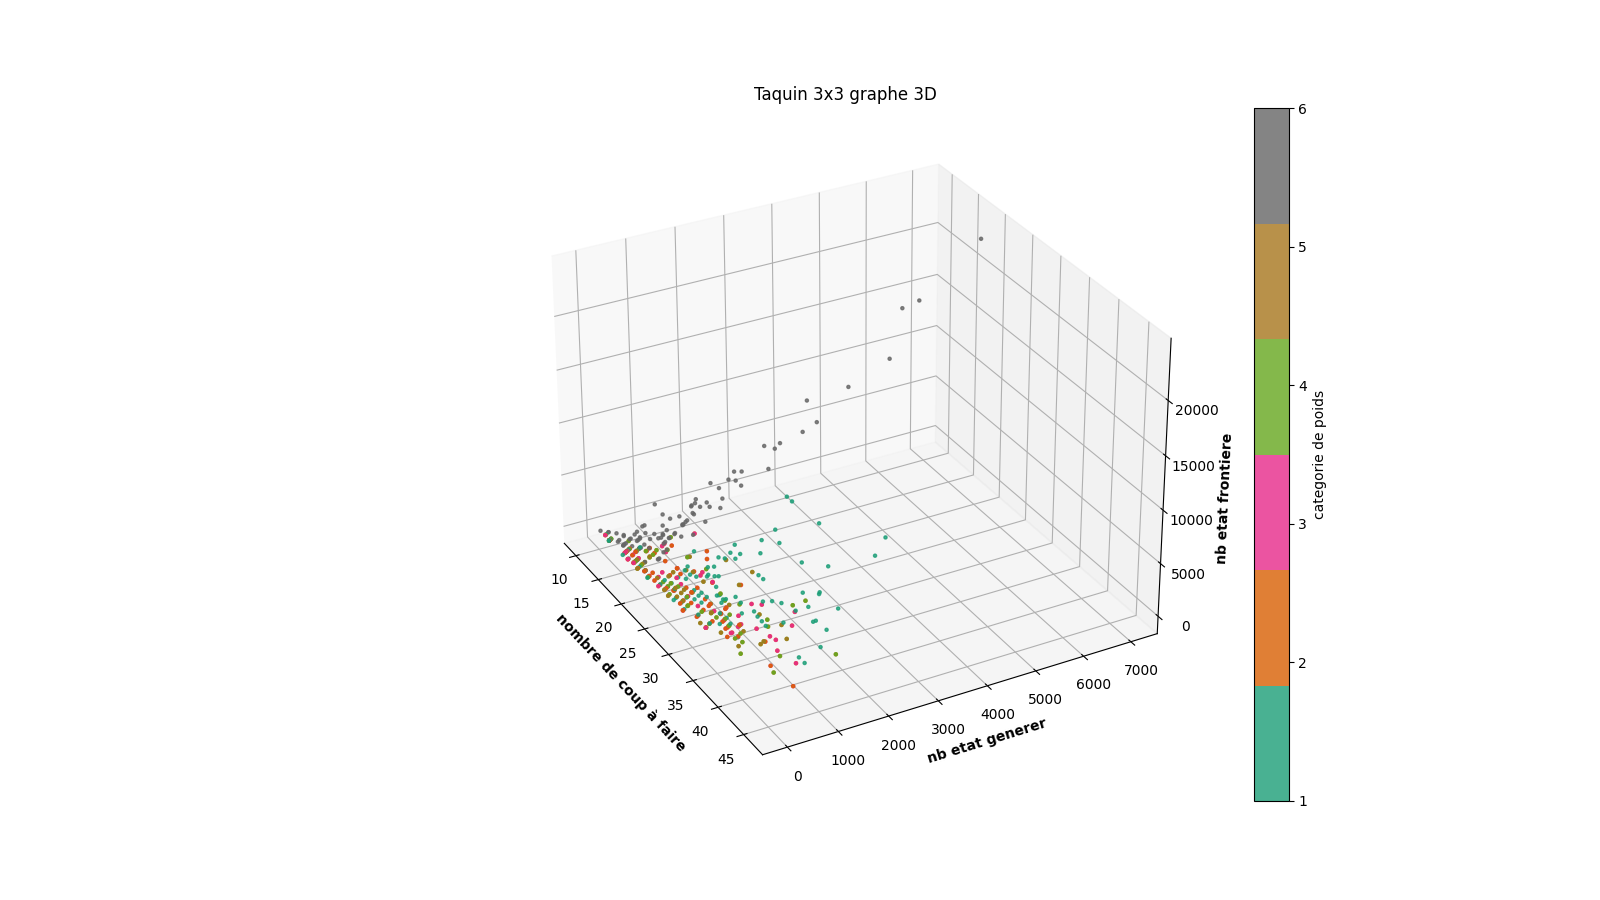
\includegraphics[width=\textwidth]{graphe 3d Taquin 3x3}
    \caption{\underline{Sans coefficiant de normalisation}}
\end{figure}
\begin{figure}[H]
    \centering
    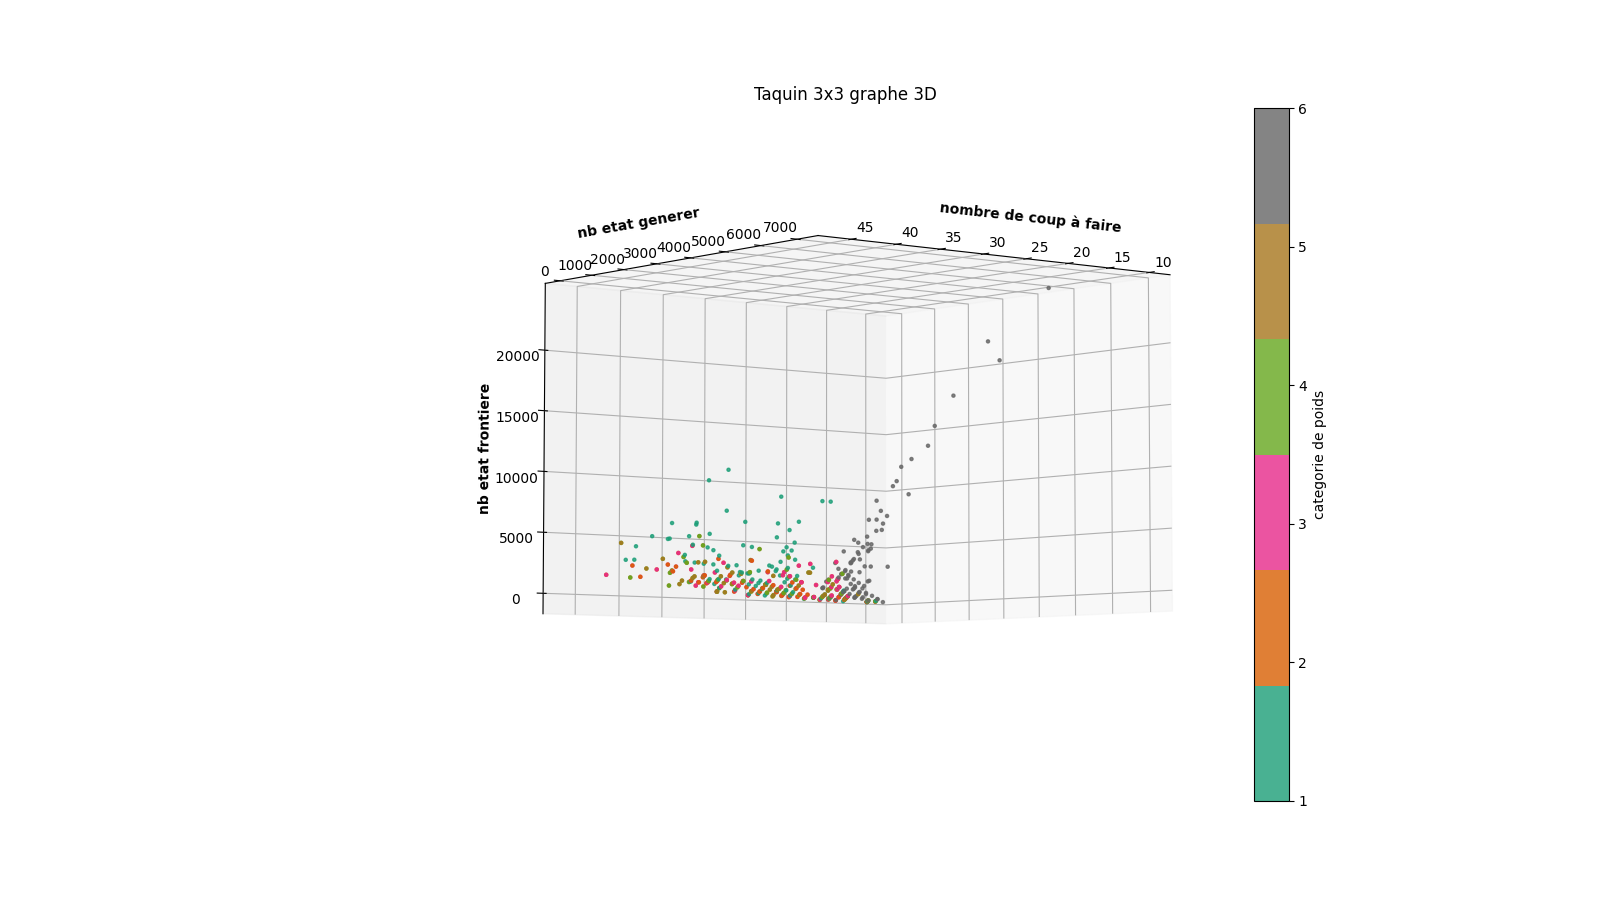
\includegraphics[width=\textwidth]{graphe 3d Taquin 3x3(1)}
    \caption{\underline{Sans coefficiant de normalisation}}
\end{figure}
\begin{figure}[H]
    \centering
    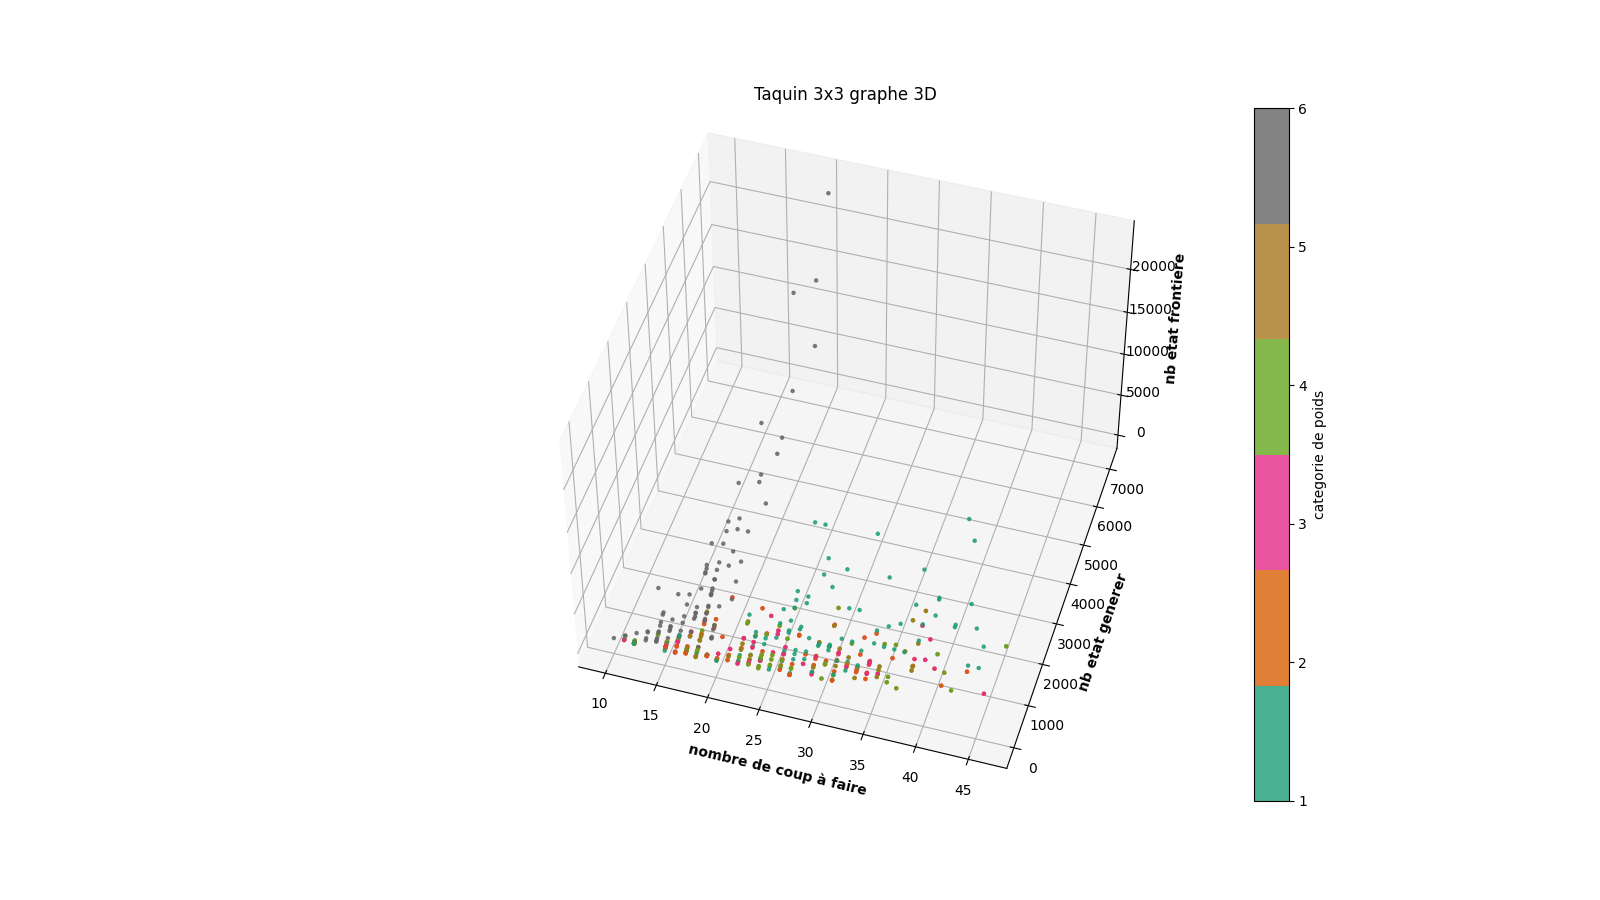
\includegraphics[width=\textwidth]{graphe 3d Taquin 3x3(2)}
    \caption{\underline{Sans coefficiant de normalisation}}
\end{figure}
\begin{figure}[H]
    \centering
    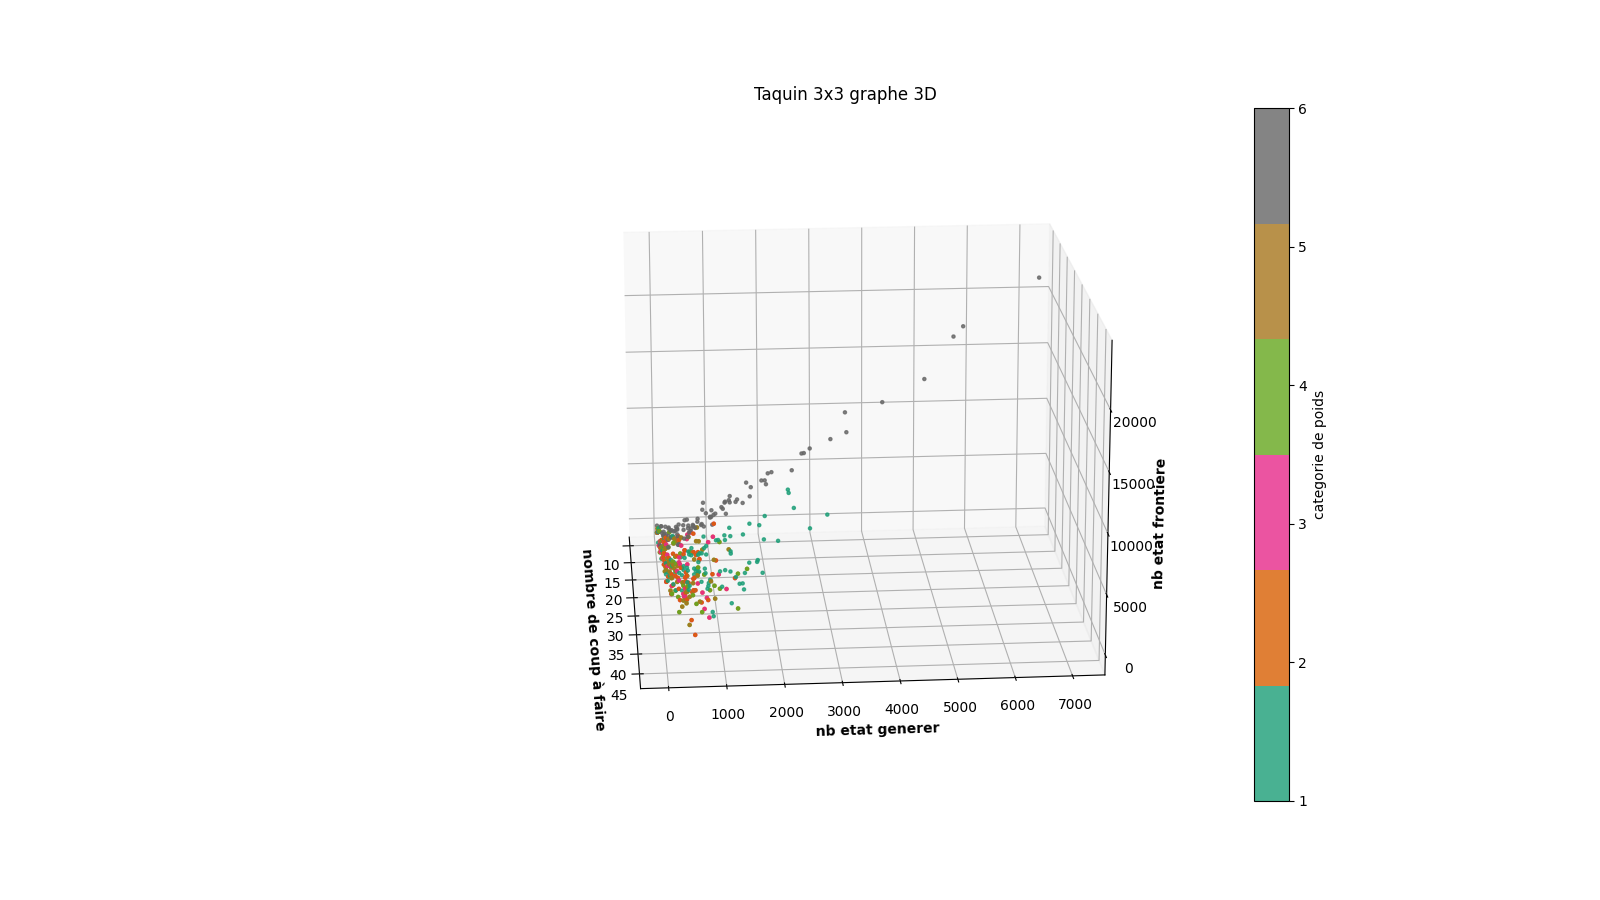
\includegraphics[width=\textwidth]{graphe 3d Taquin 3x3(3)}
    \caption{\underline{Sans coefficiant de normalisation}}
\end{figure}

\begin{figure}[H]
    \centering
    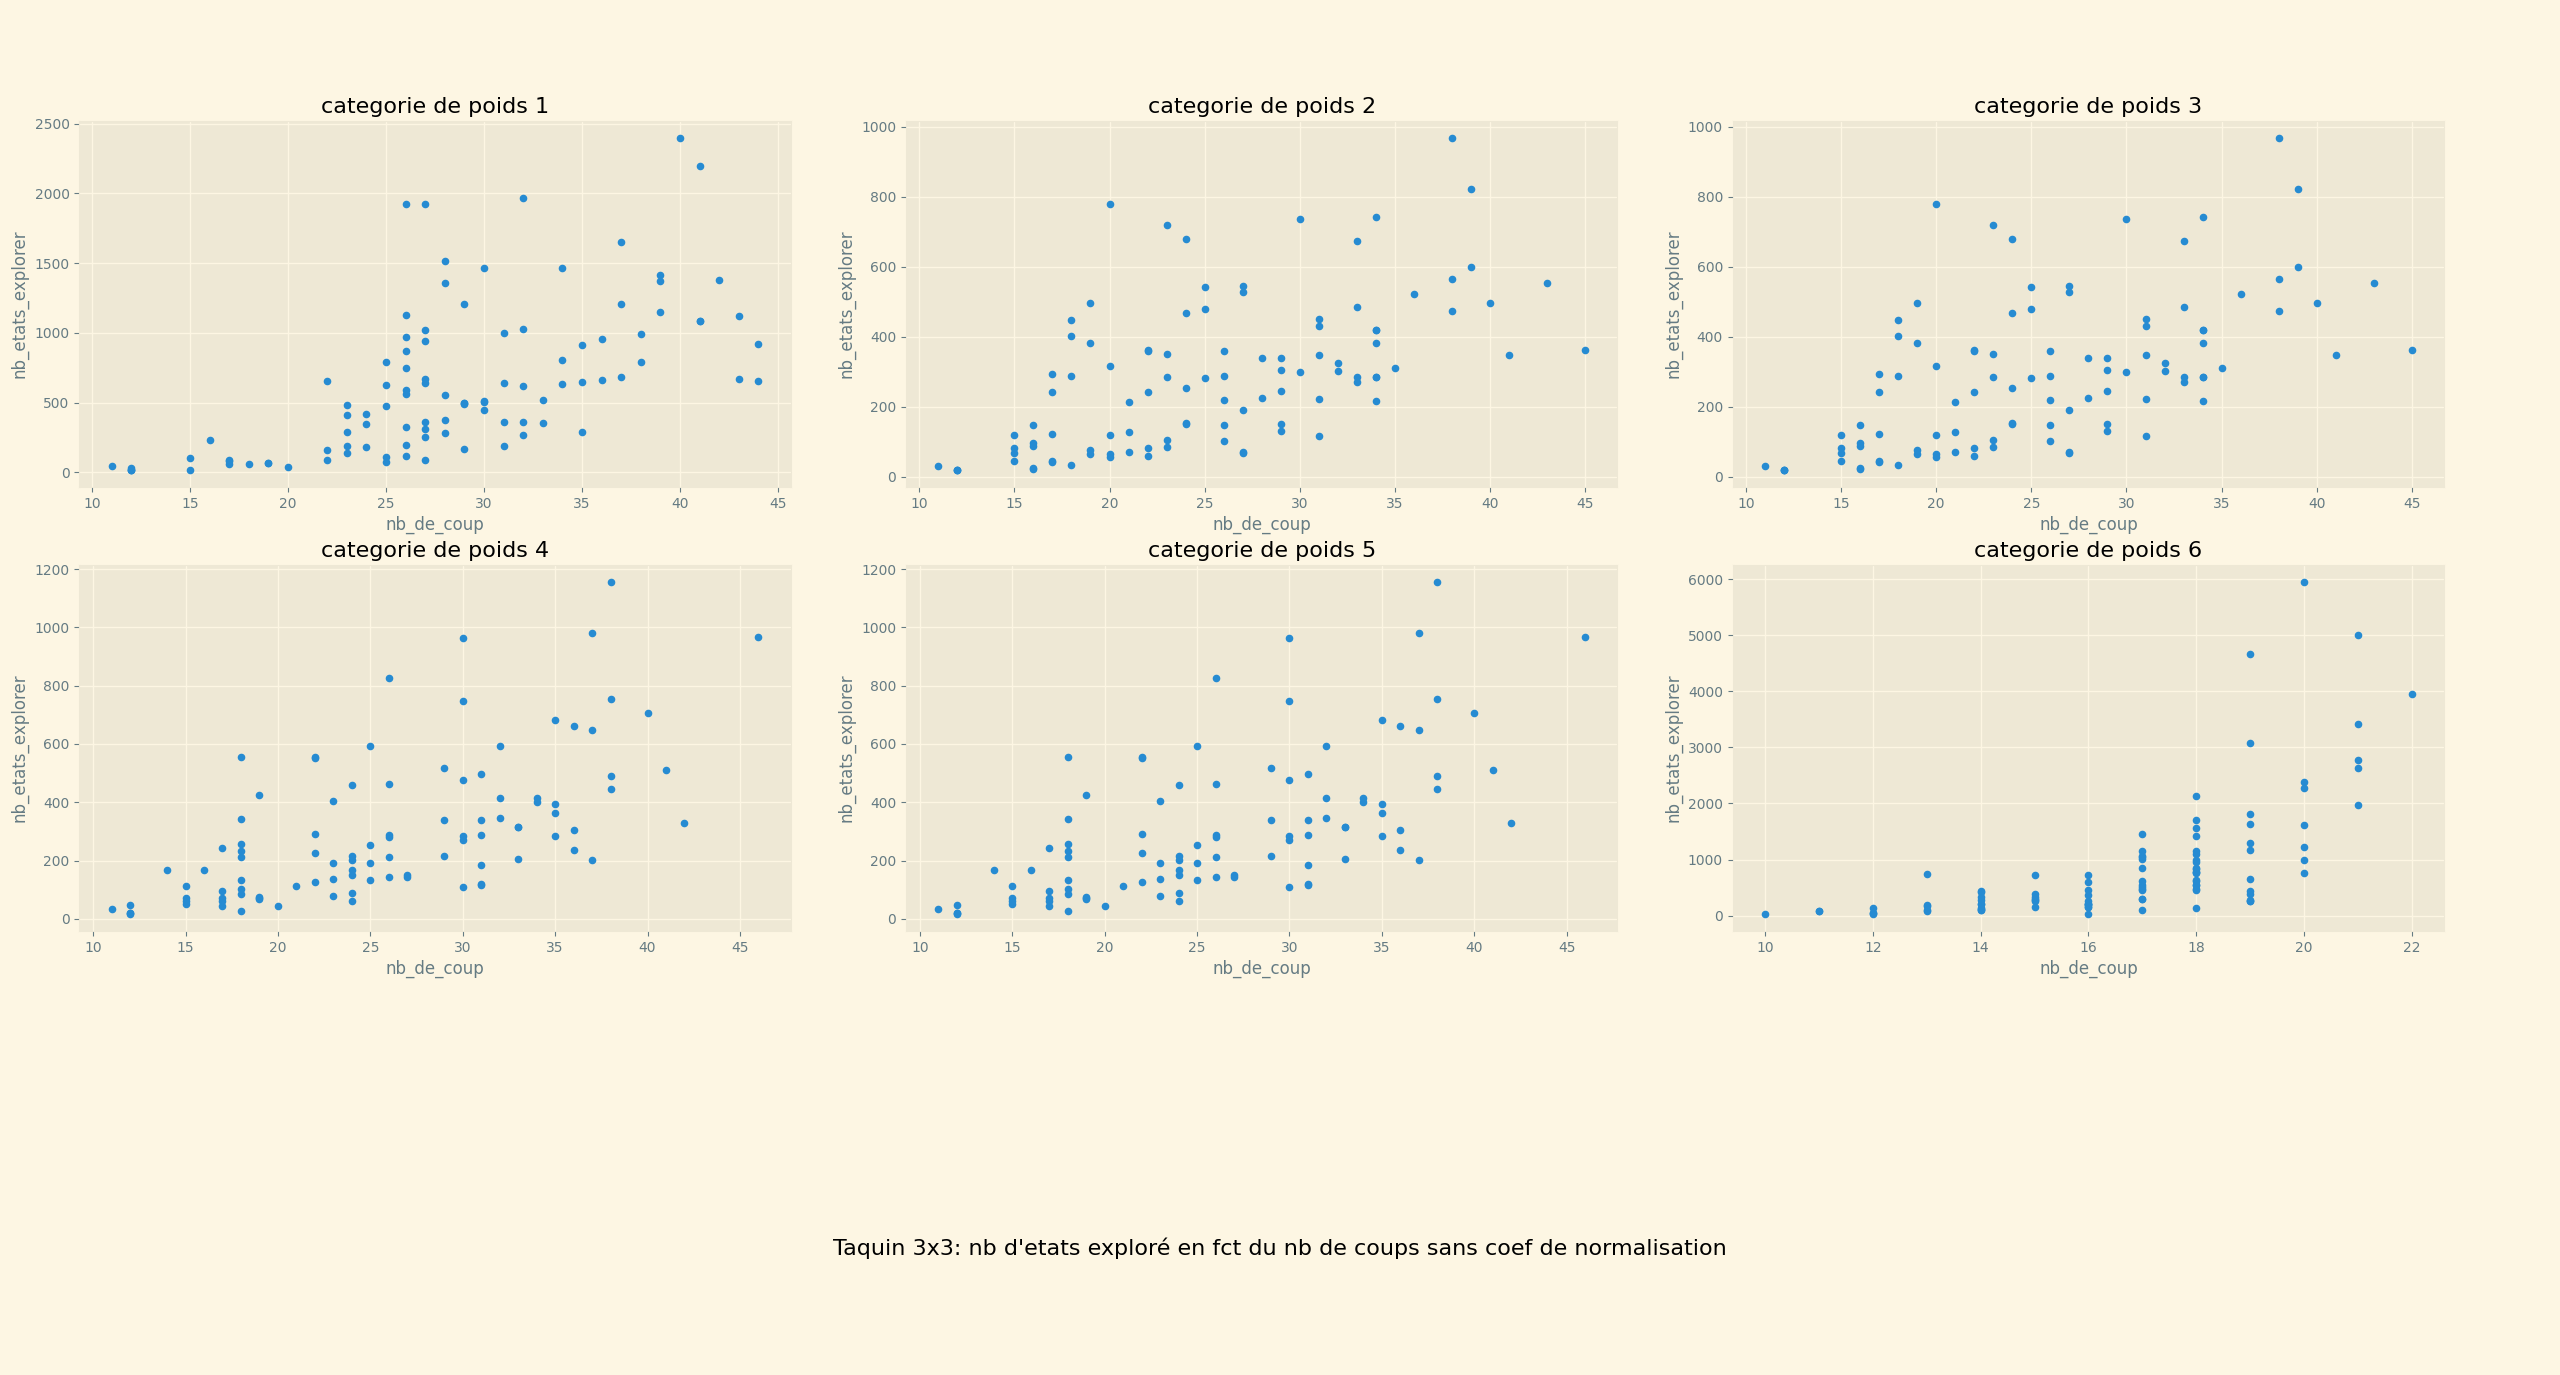
\includegraphics[width=\textwidth]{Taquin 3x3 nombre d'etat explorer en fct du nb de coups sans coef}
\end{figure}

\begin{figure}[H]
    \centering
    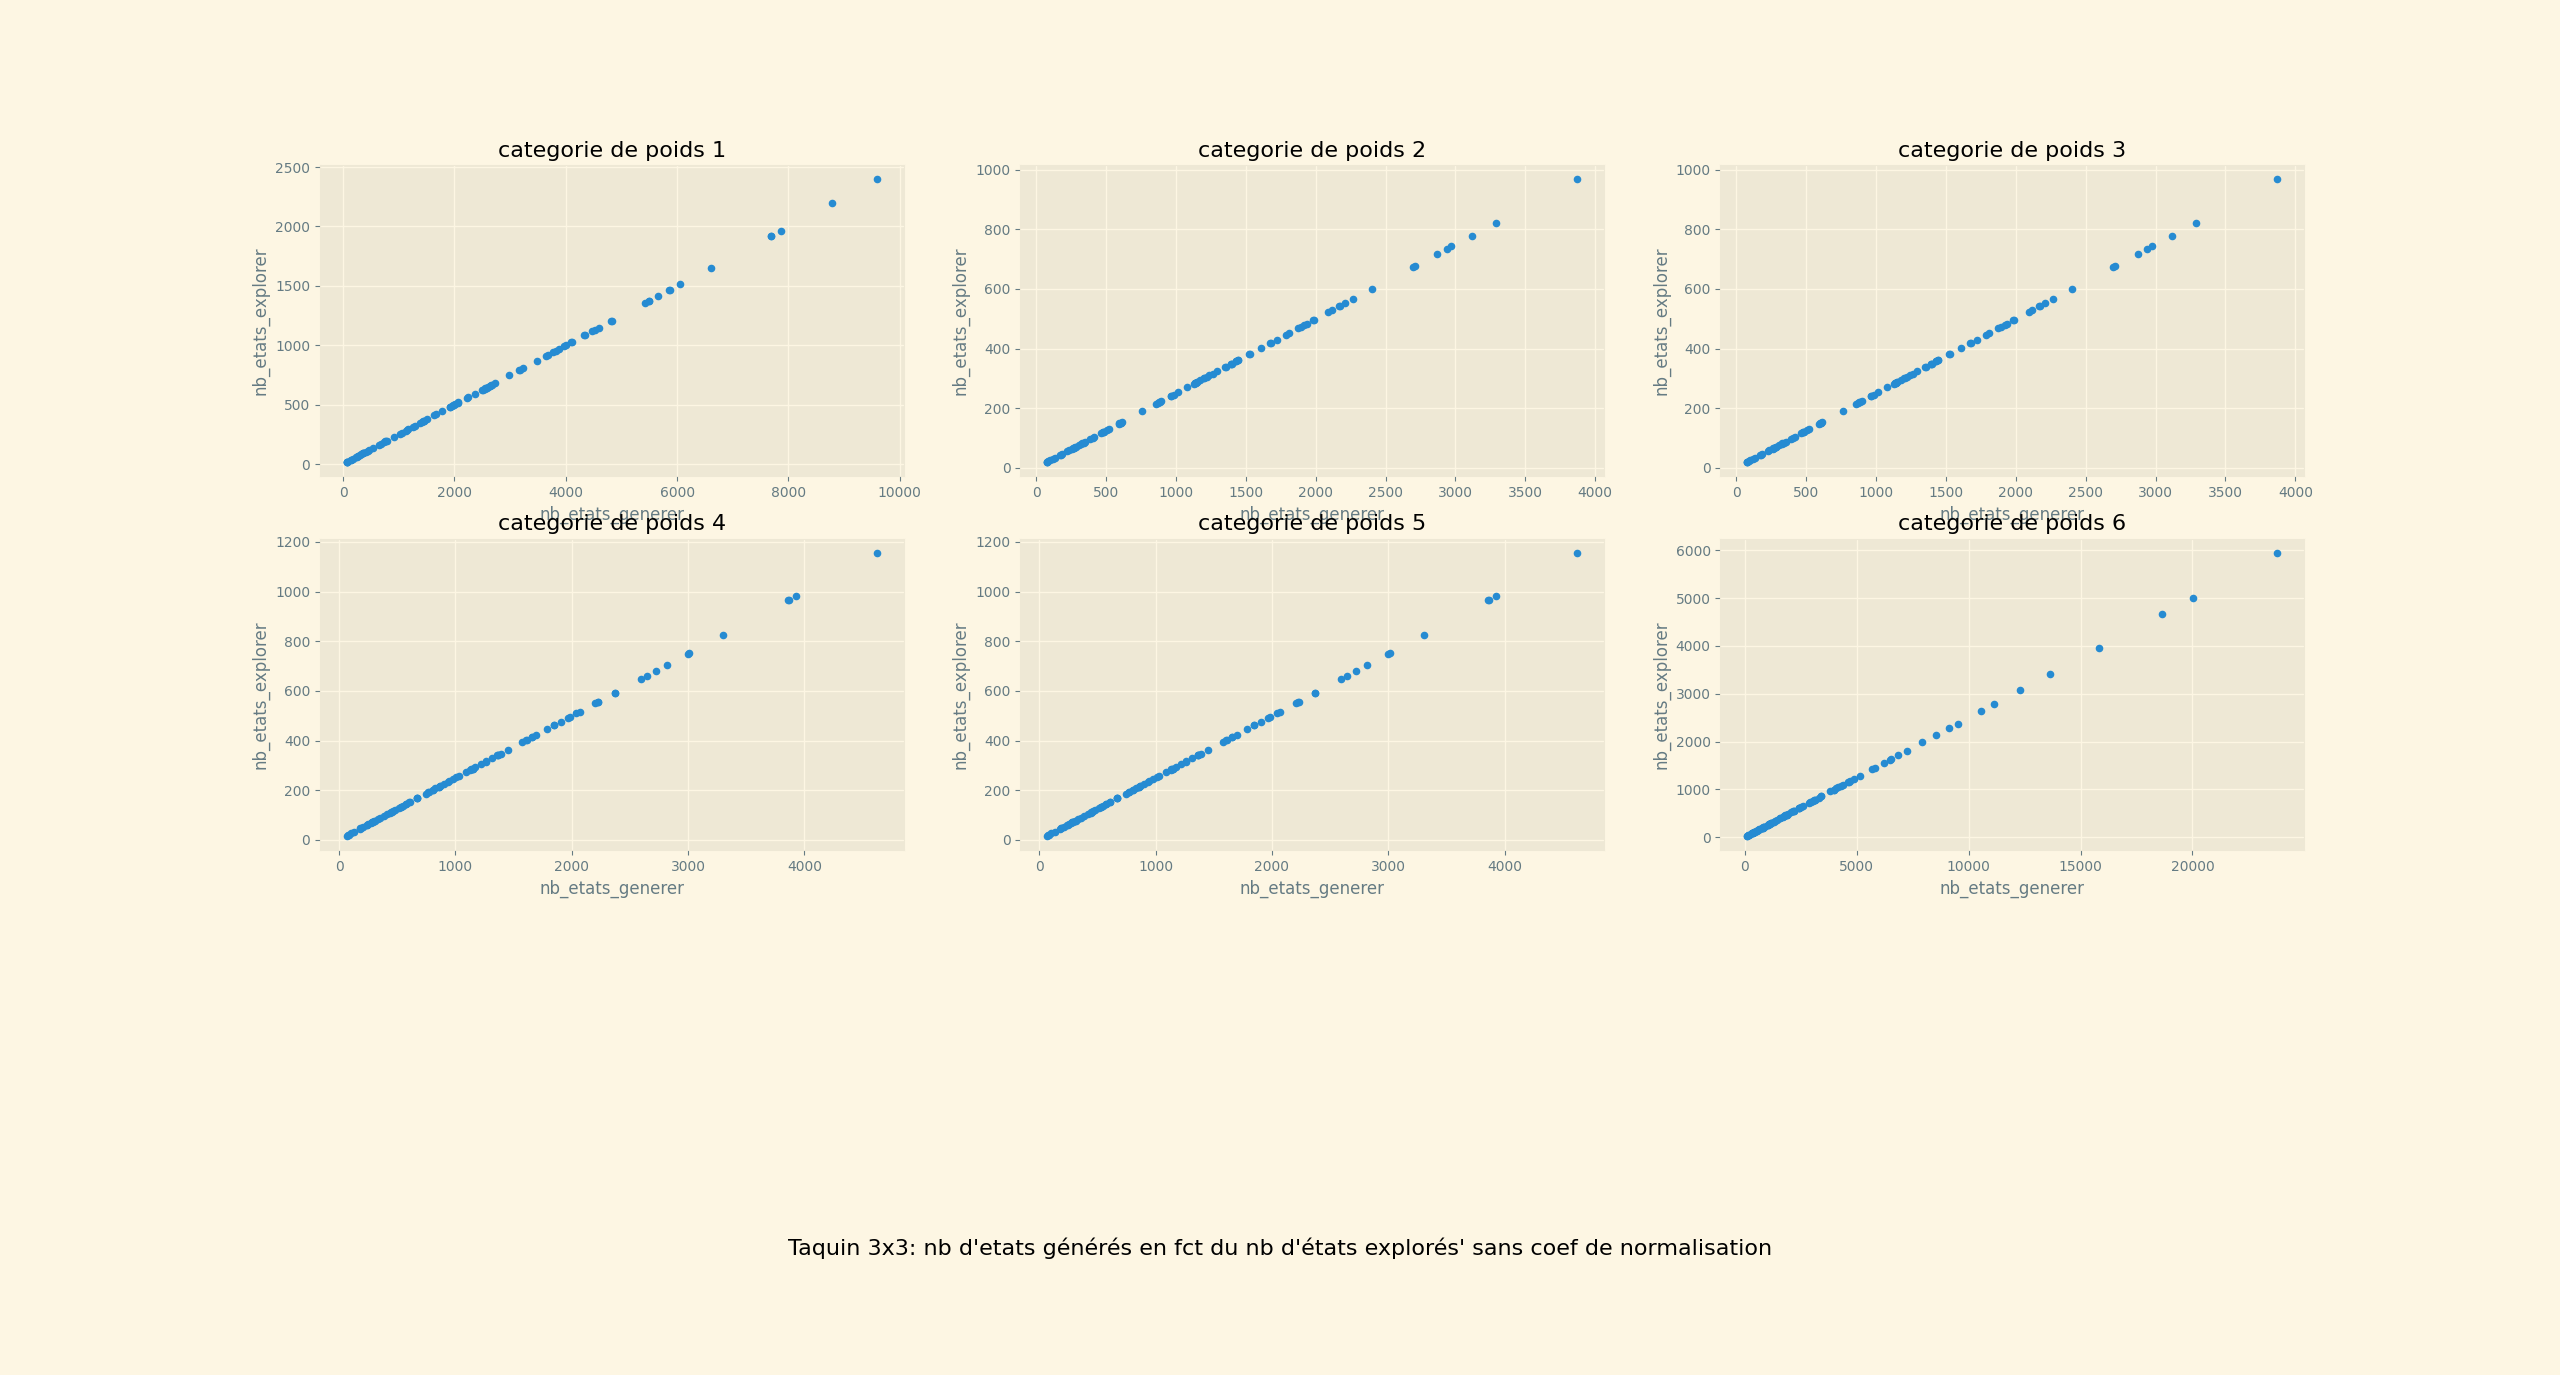
\includegraphics[width=\textwidth]{Taquin 3x3 nombre d'etats generer en fct du nb d etat explorer sans coef}
\end{figure}

\begin{figure}[H]
    \centering
    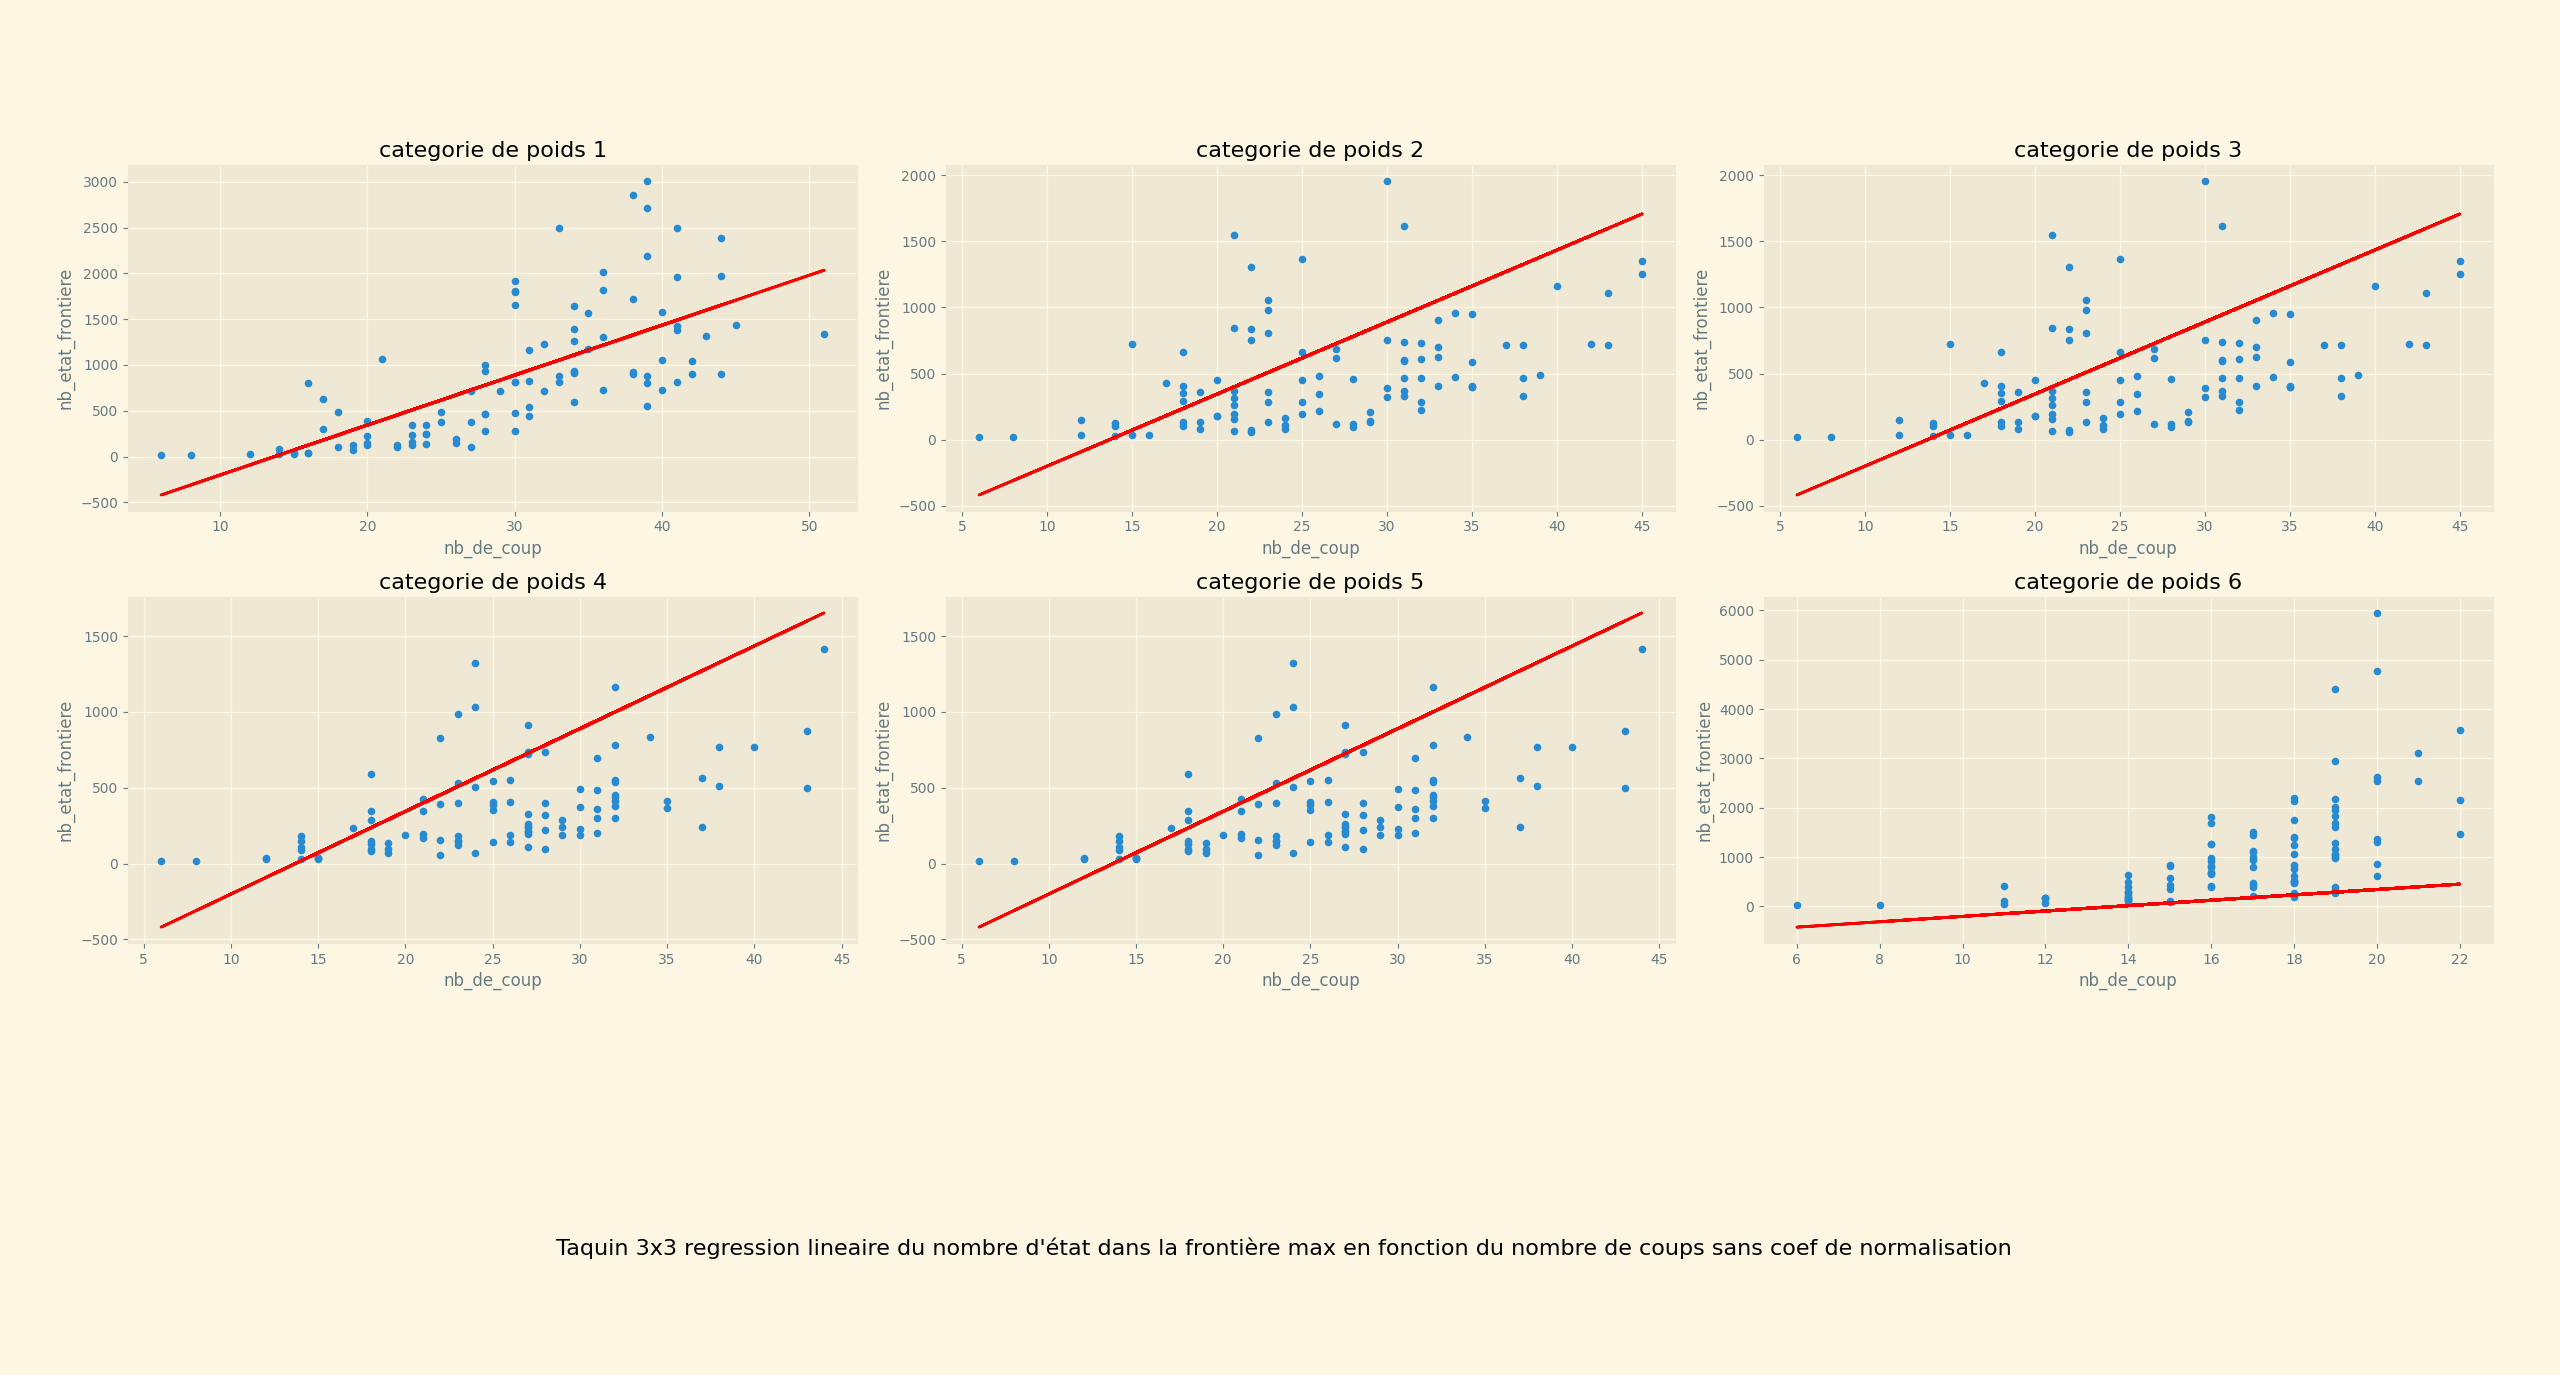
\includegraphics[width=\textwidth]{Taquin 3x3 regression lineaire du nombre d'état dans la frontière max en fonction du nombre de coups sans coef de normalisation}
\end{figure}

\begin{figure}[H]
    \centering
    \includegraphics[width=\textwidth]{Taquin 3x3 regression lineaire du nombre d'état explorer en fonction du nombre de coups sans coef de normalisation}
\end{figure}

\begin{figure}[H]
    \centering
    \includegraphics[width=\textwidth]{Taquin 3x3 regression lineaire du nombre d'état generer en fonction du nombre de coups sans coef de normalisation}
\end{figure}

\begin{figure}[H]
    \centering
    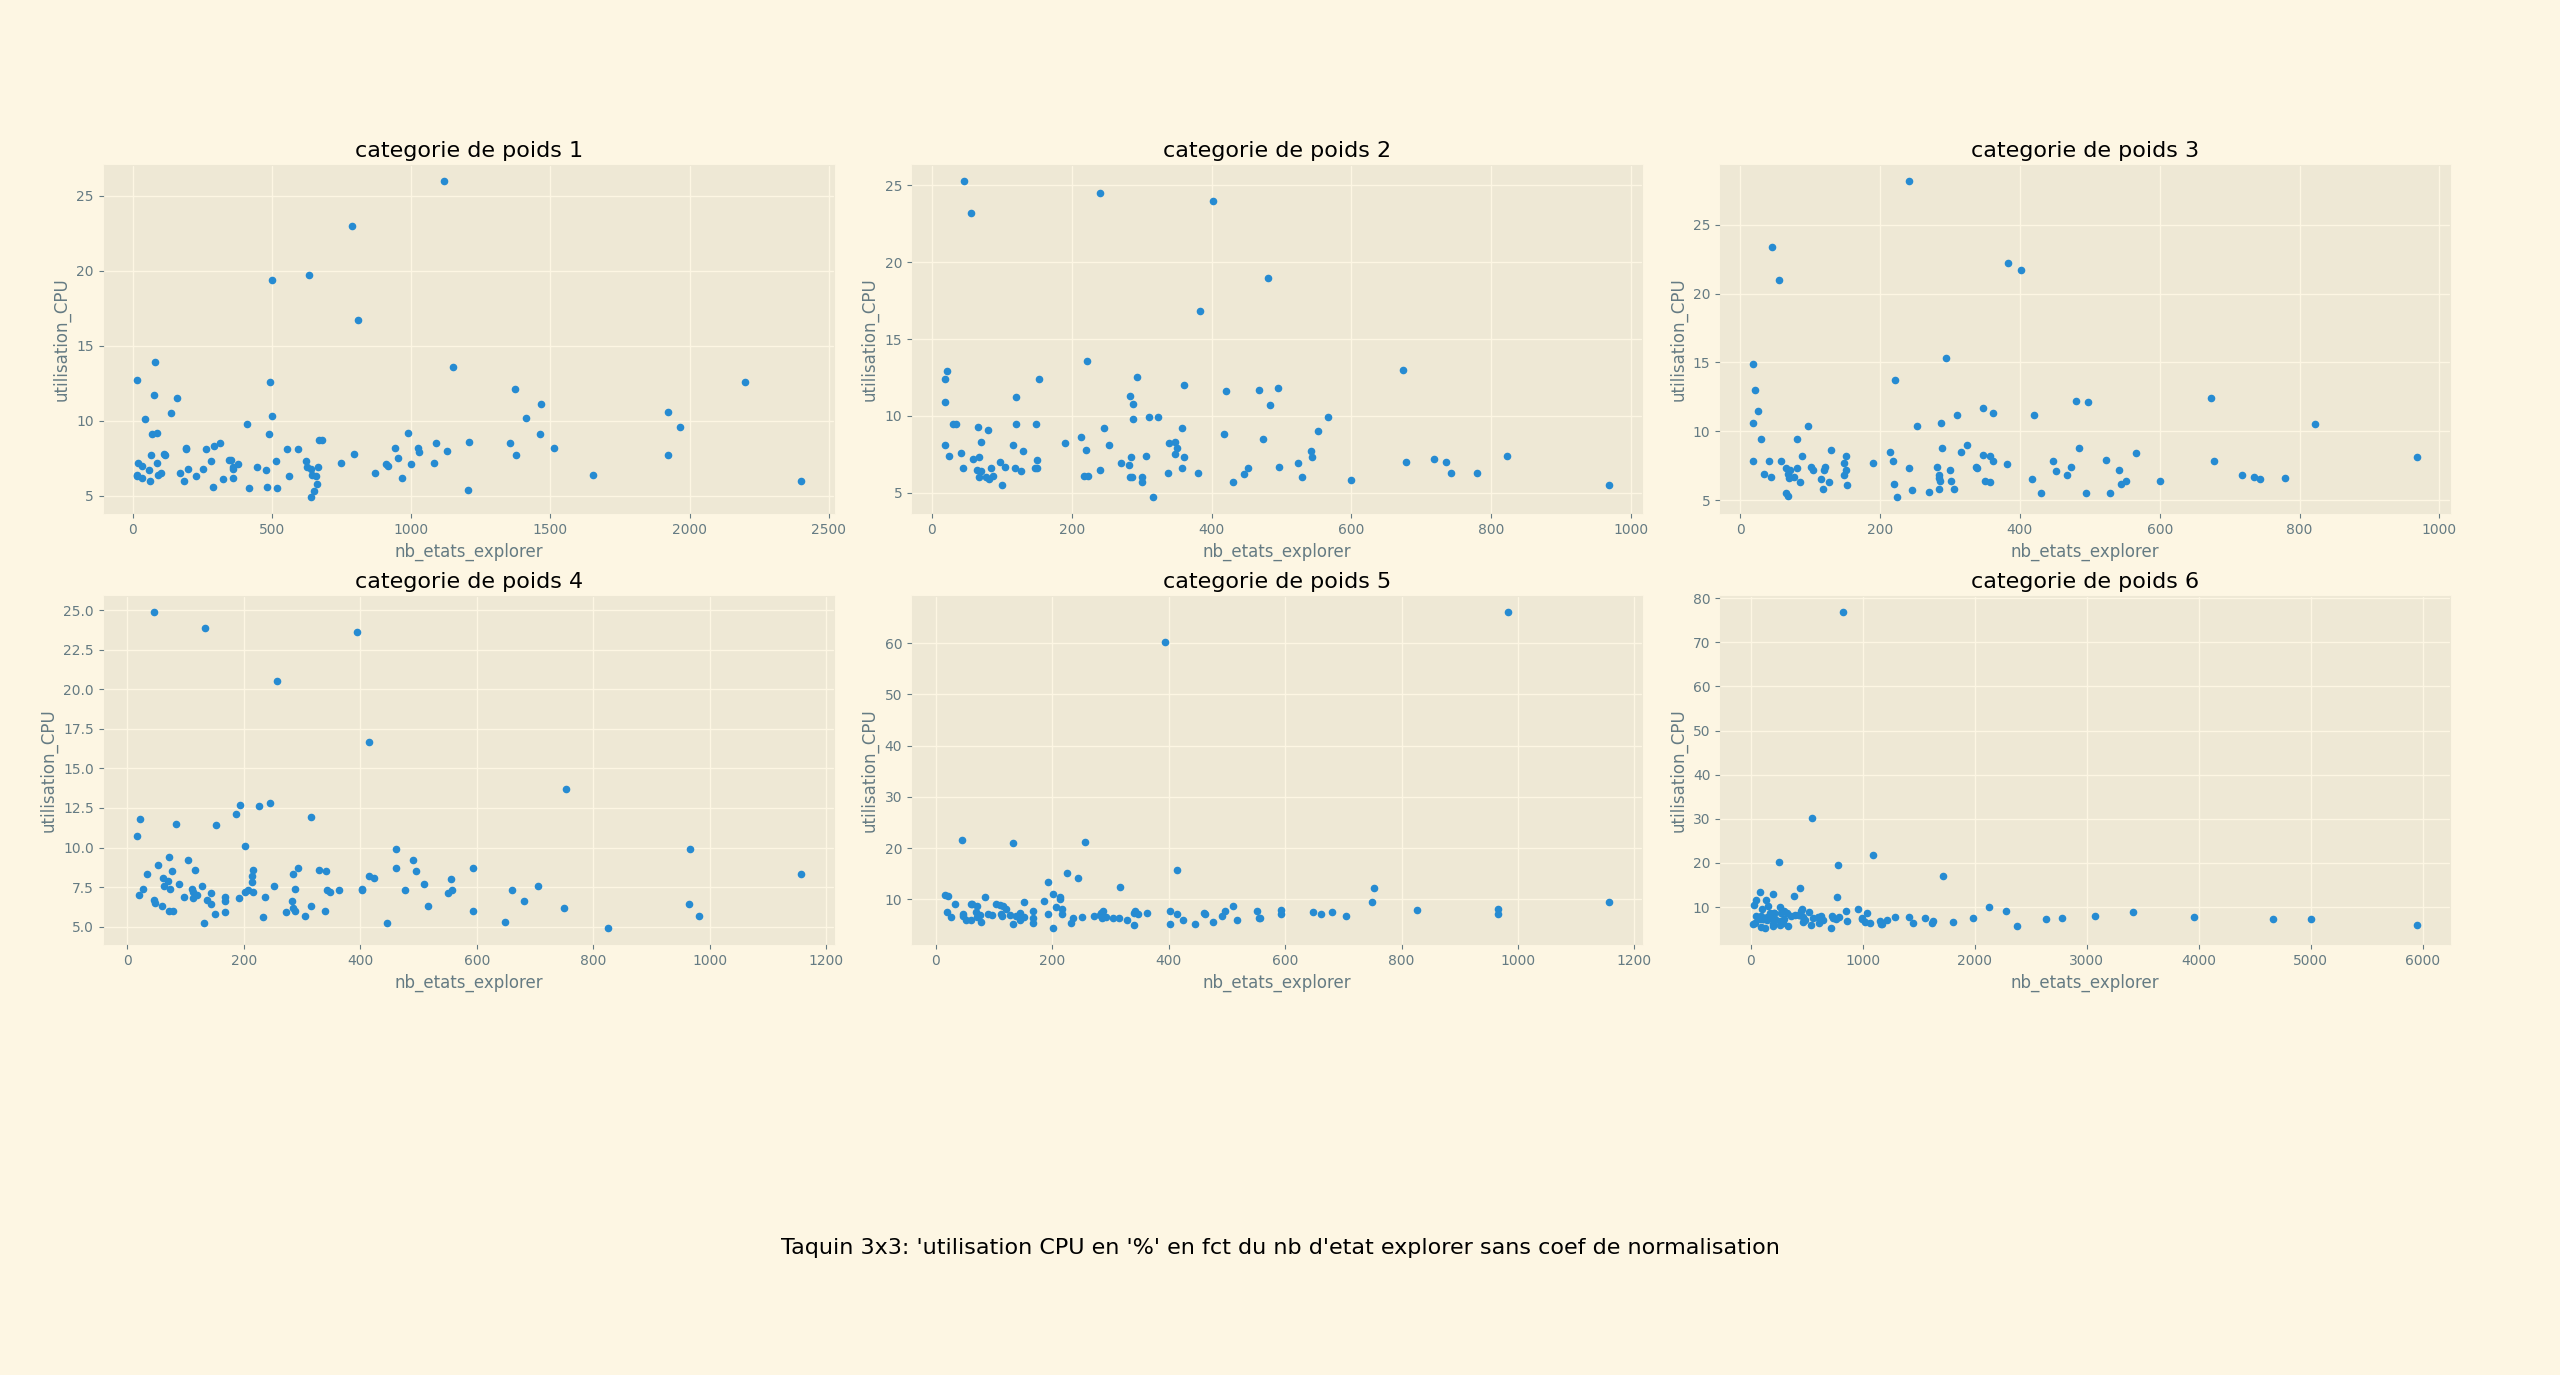
\includegraphics[width=\textwidth]{Taquin 3x3 utilisation CPU en fct du nb d'etat explorer sans coef de normalisation}
\end{figure}

\begin{figure}[H]
    \centering
    \includegraphics[width=\textwidth]{Taquin 3x3 nombre d'état explorer en fct du nb detat ds la frontiere sans coef}
\end{figure}

\begin{figure}[H]
    \centering
    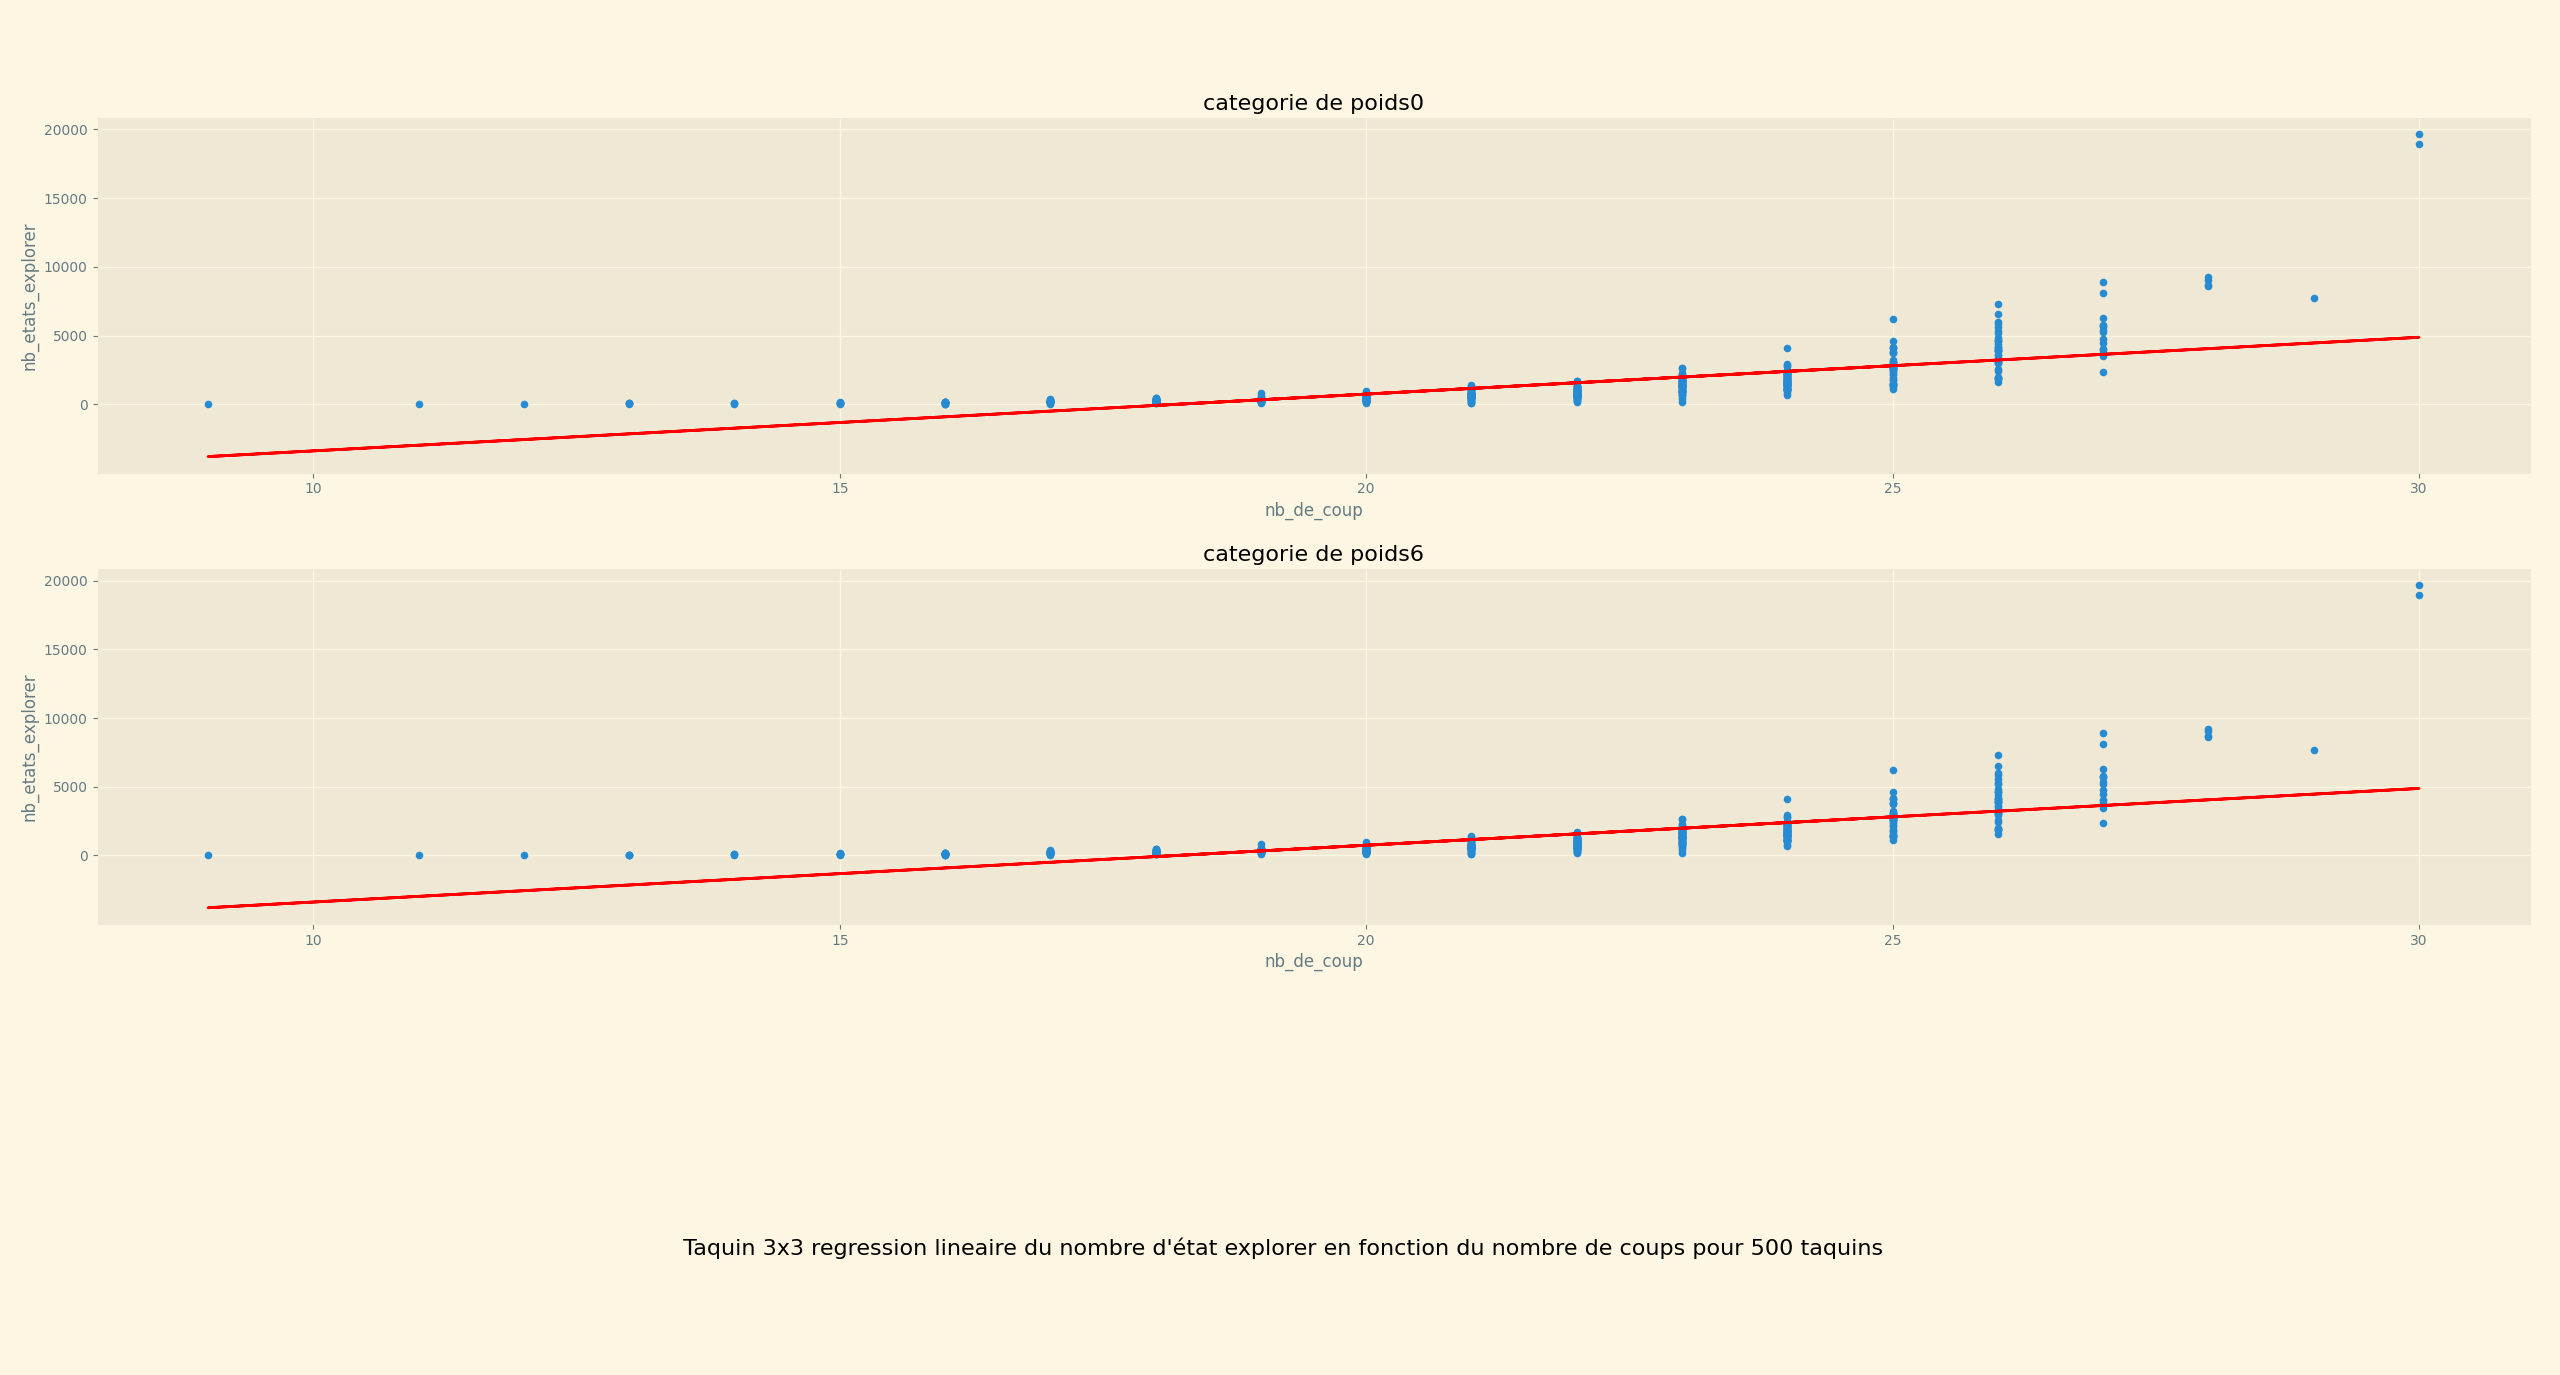
\includegraphics[width=\textwidth]{Taquin 3x3 nombre d'etat explorer en fct du nb de coups}
\end{figure}

\begin{figure}[H]
    \centering
    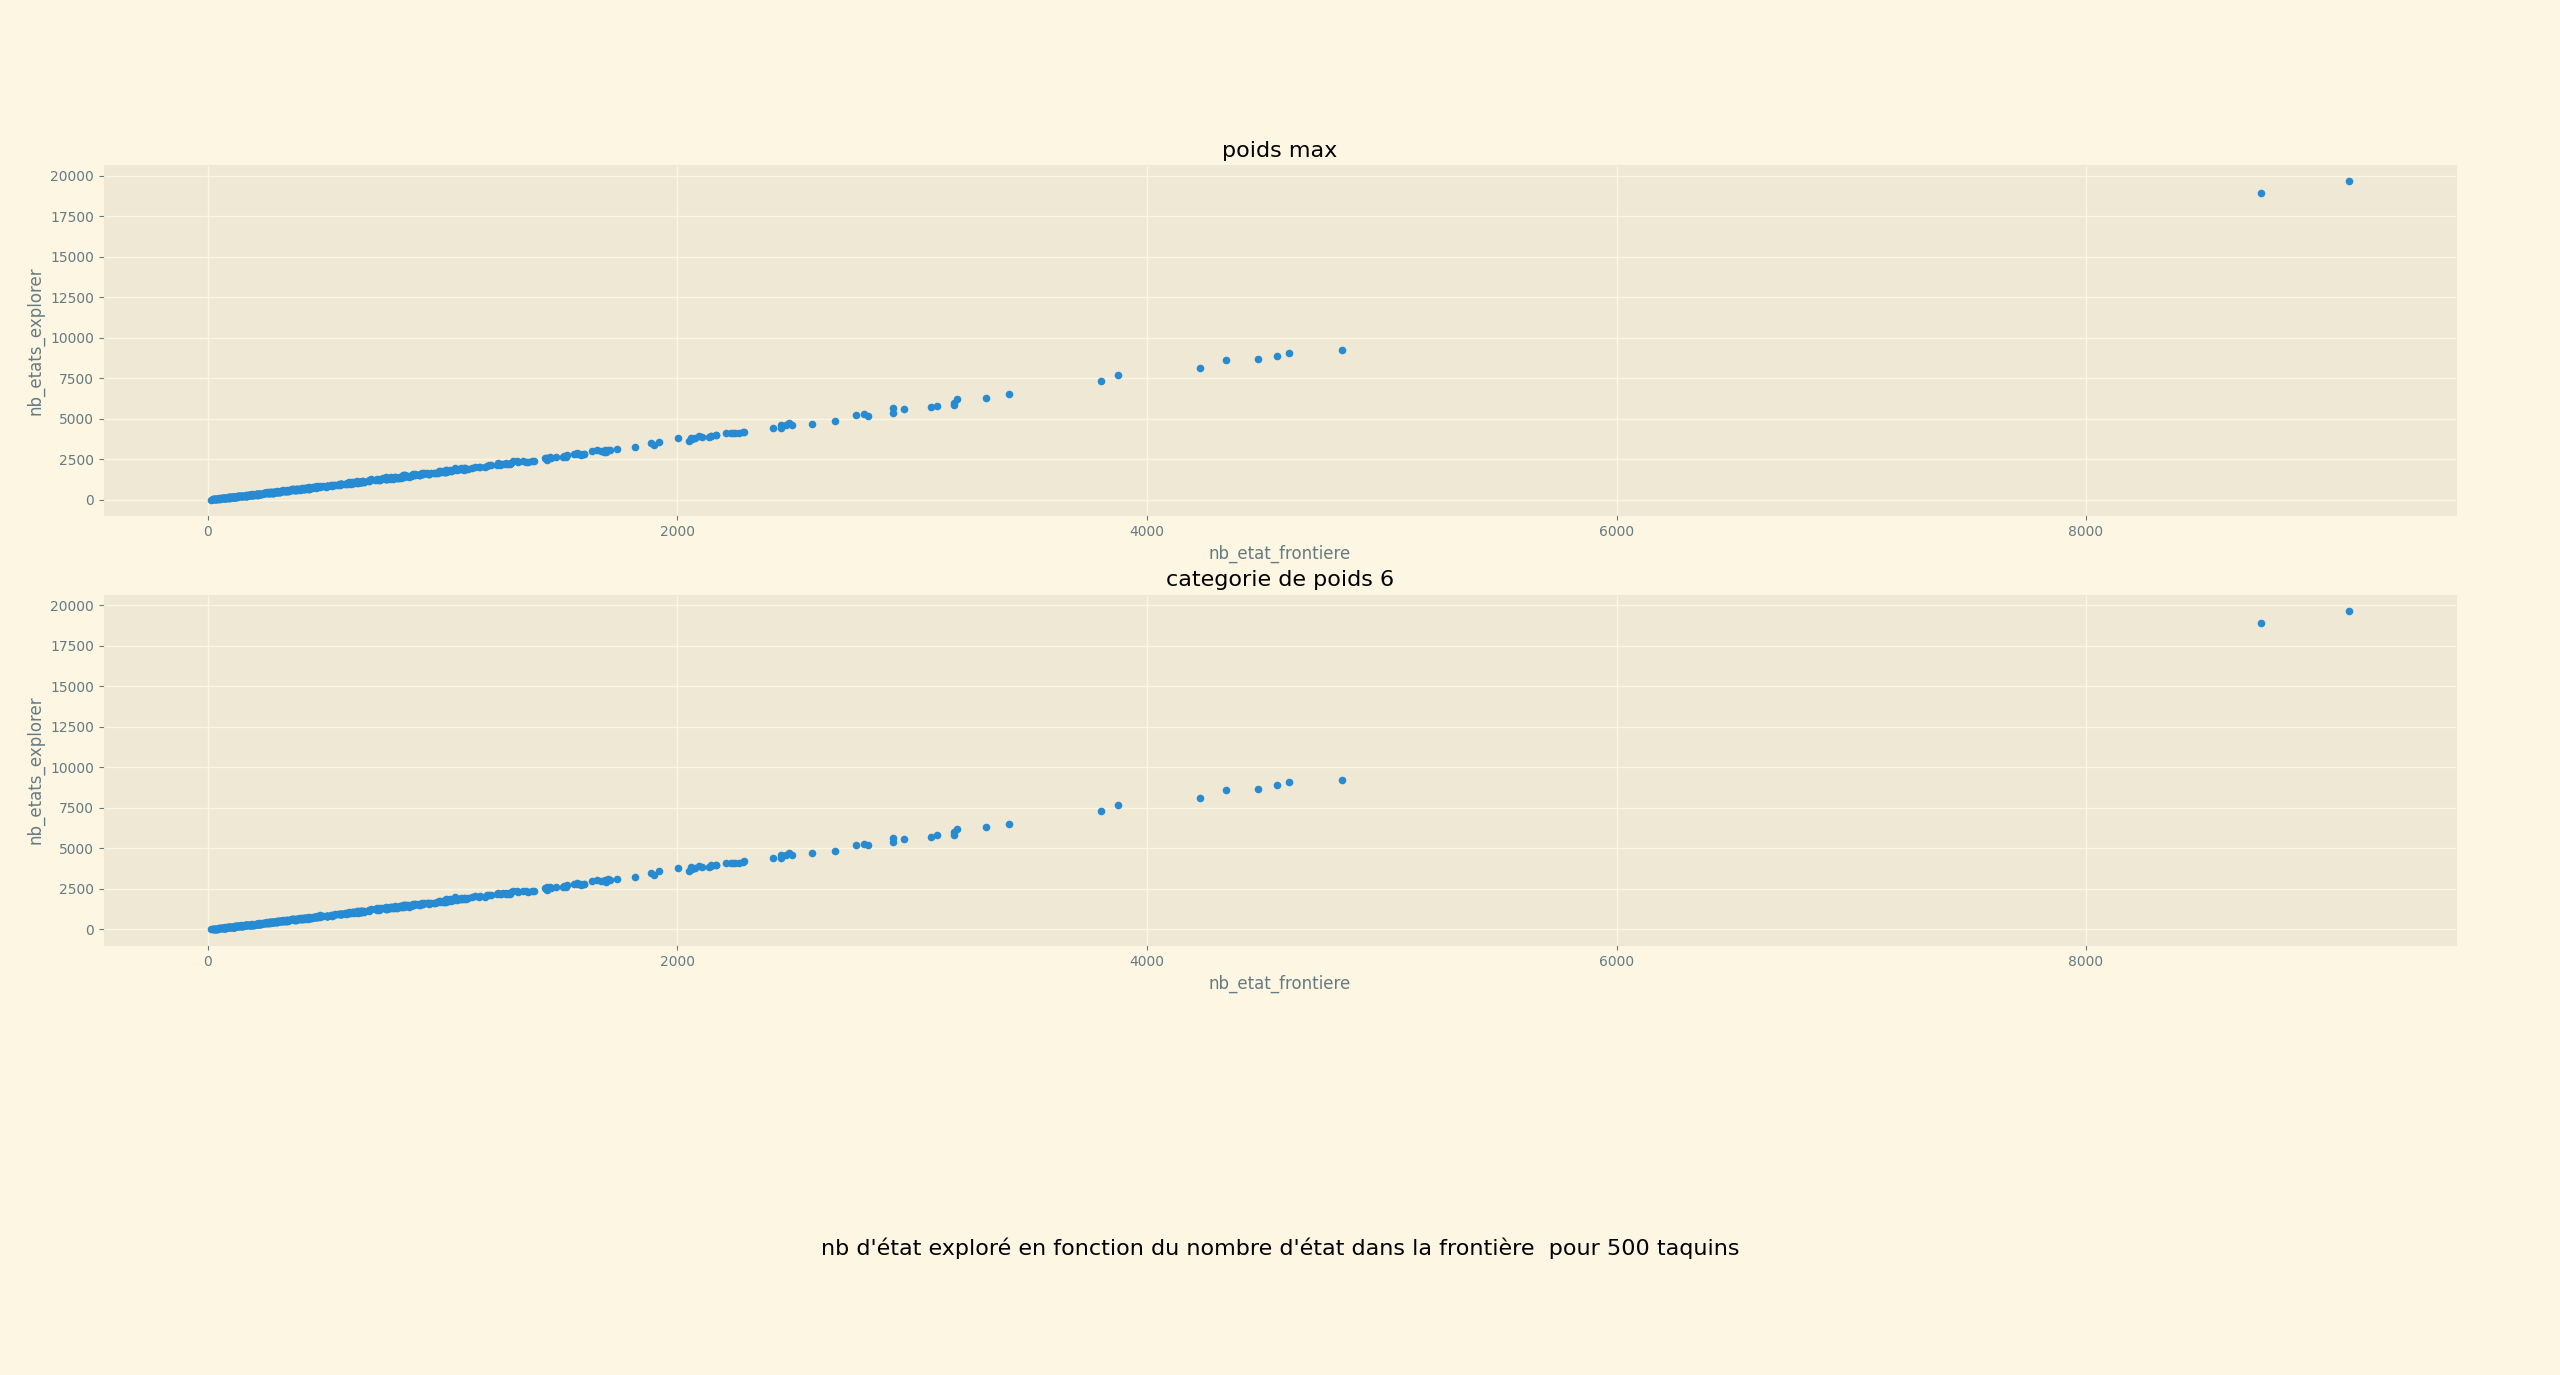
\includegraphics[width=\textwidth]{Taquin 3x3 nombre d'etat explorer en fct du nb de detat dans la frontiere}
\end{figure}

\begin{figure}[H]
    \centering
    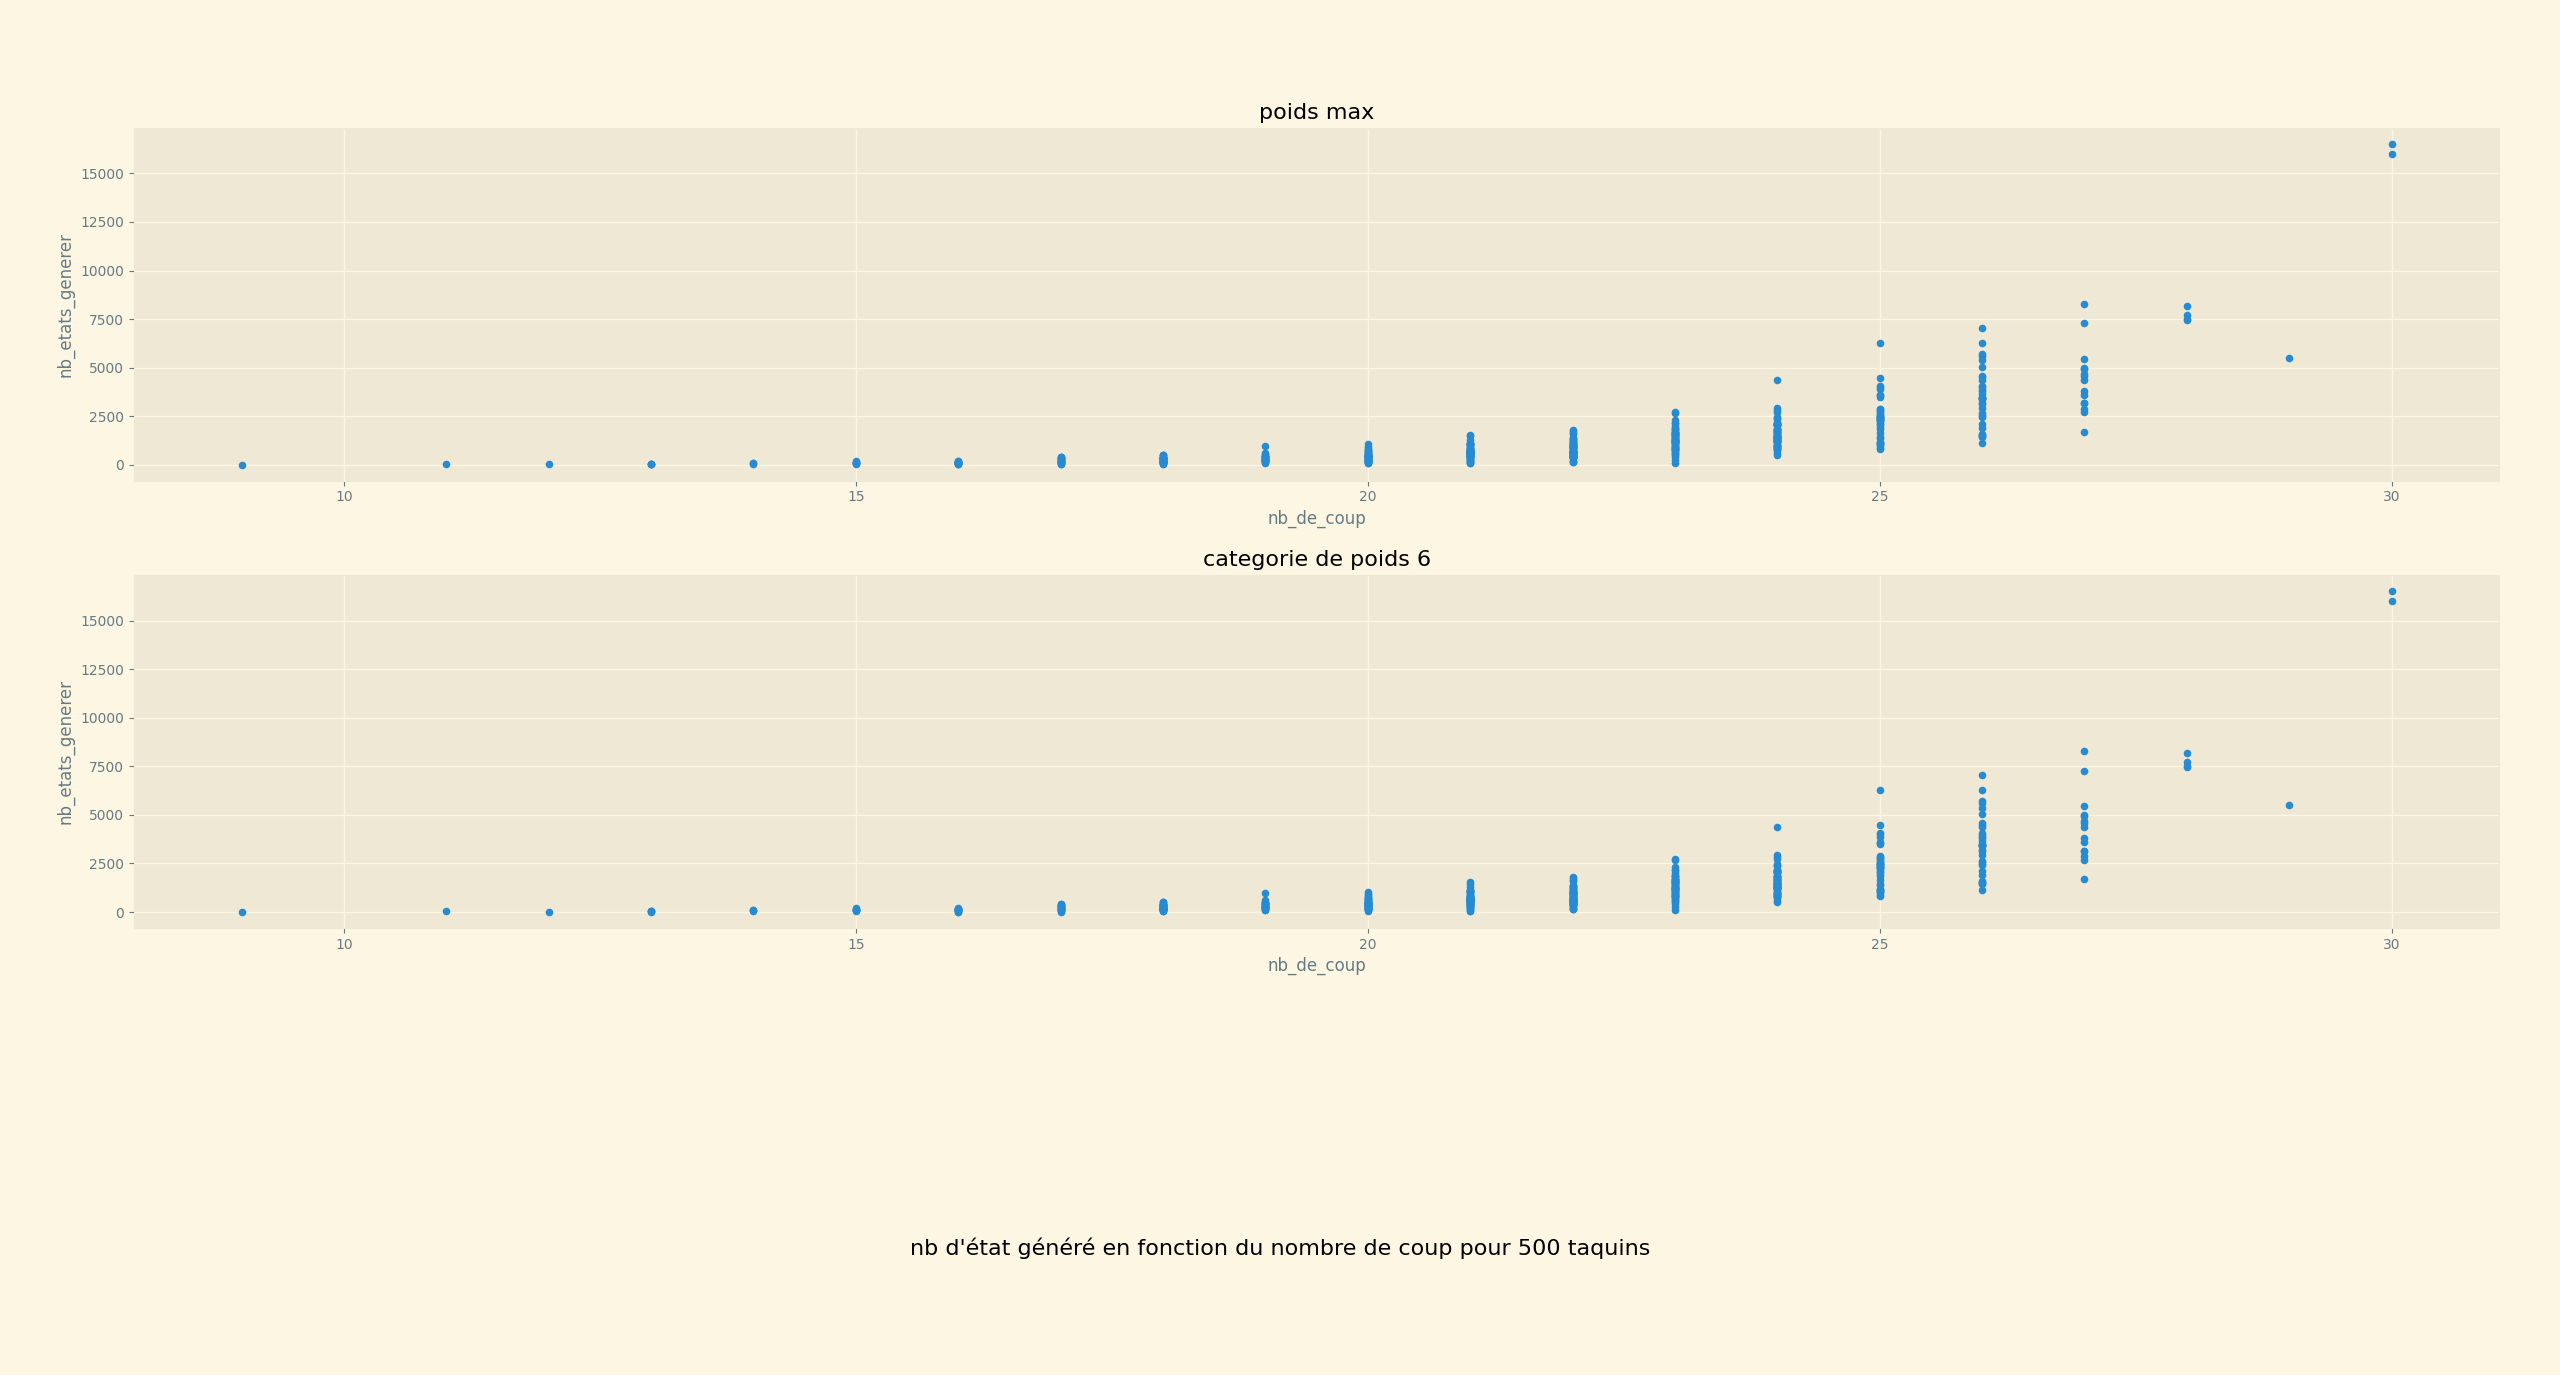
\includegraphics[width=\textwidth]{Taquin 3x3 nombre d'etats generer en fct du nb de coups}
\end{figure}

\begin{figure}[H]
    \centering
    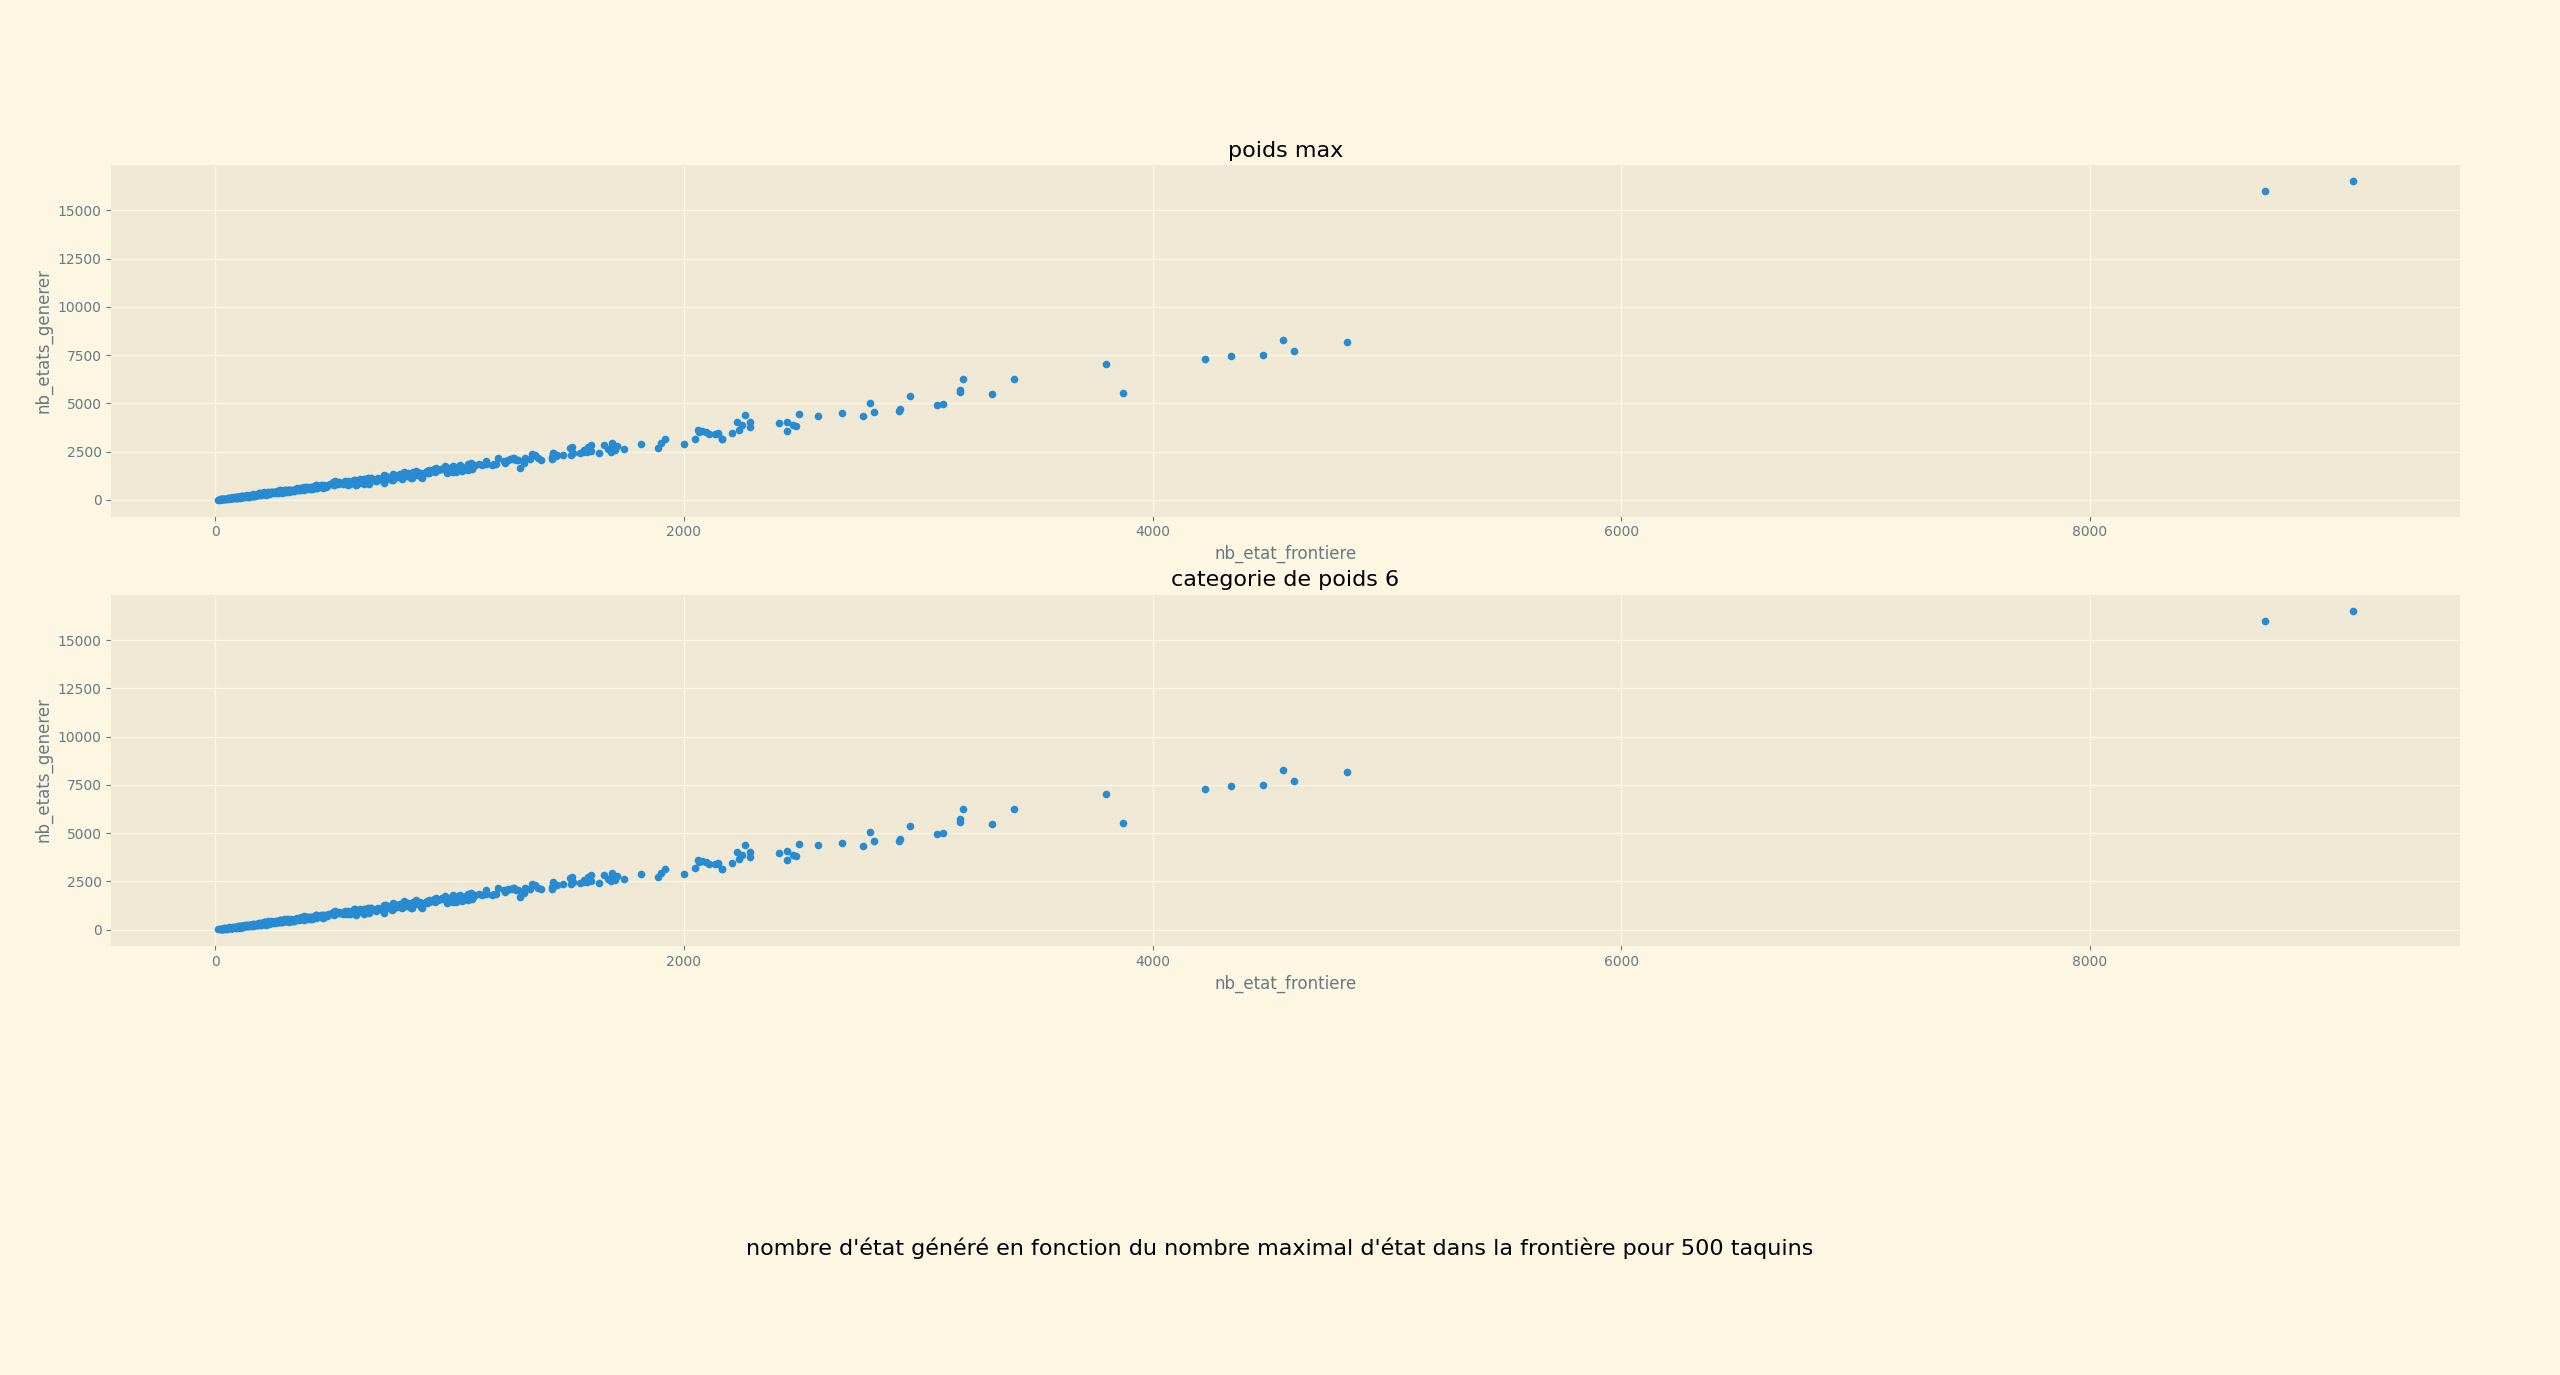
\includegraphics[width=\textwidth]{Taquin 3x3 nombre d'etats generer en fct du nb max detat dans la frontiere}
\end{figure}

\begin{figure}[H]
    \centering
    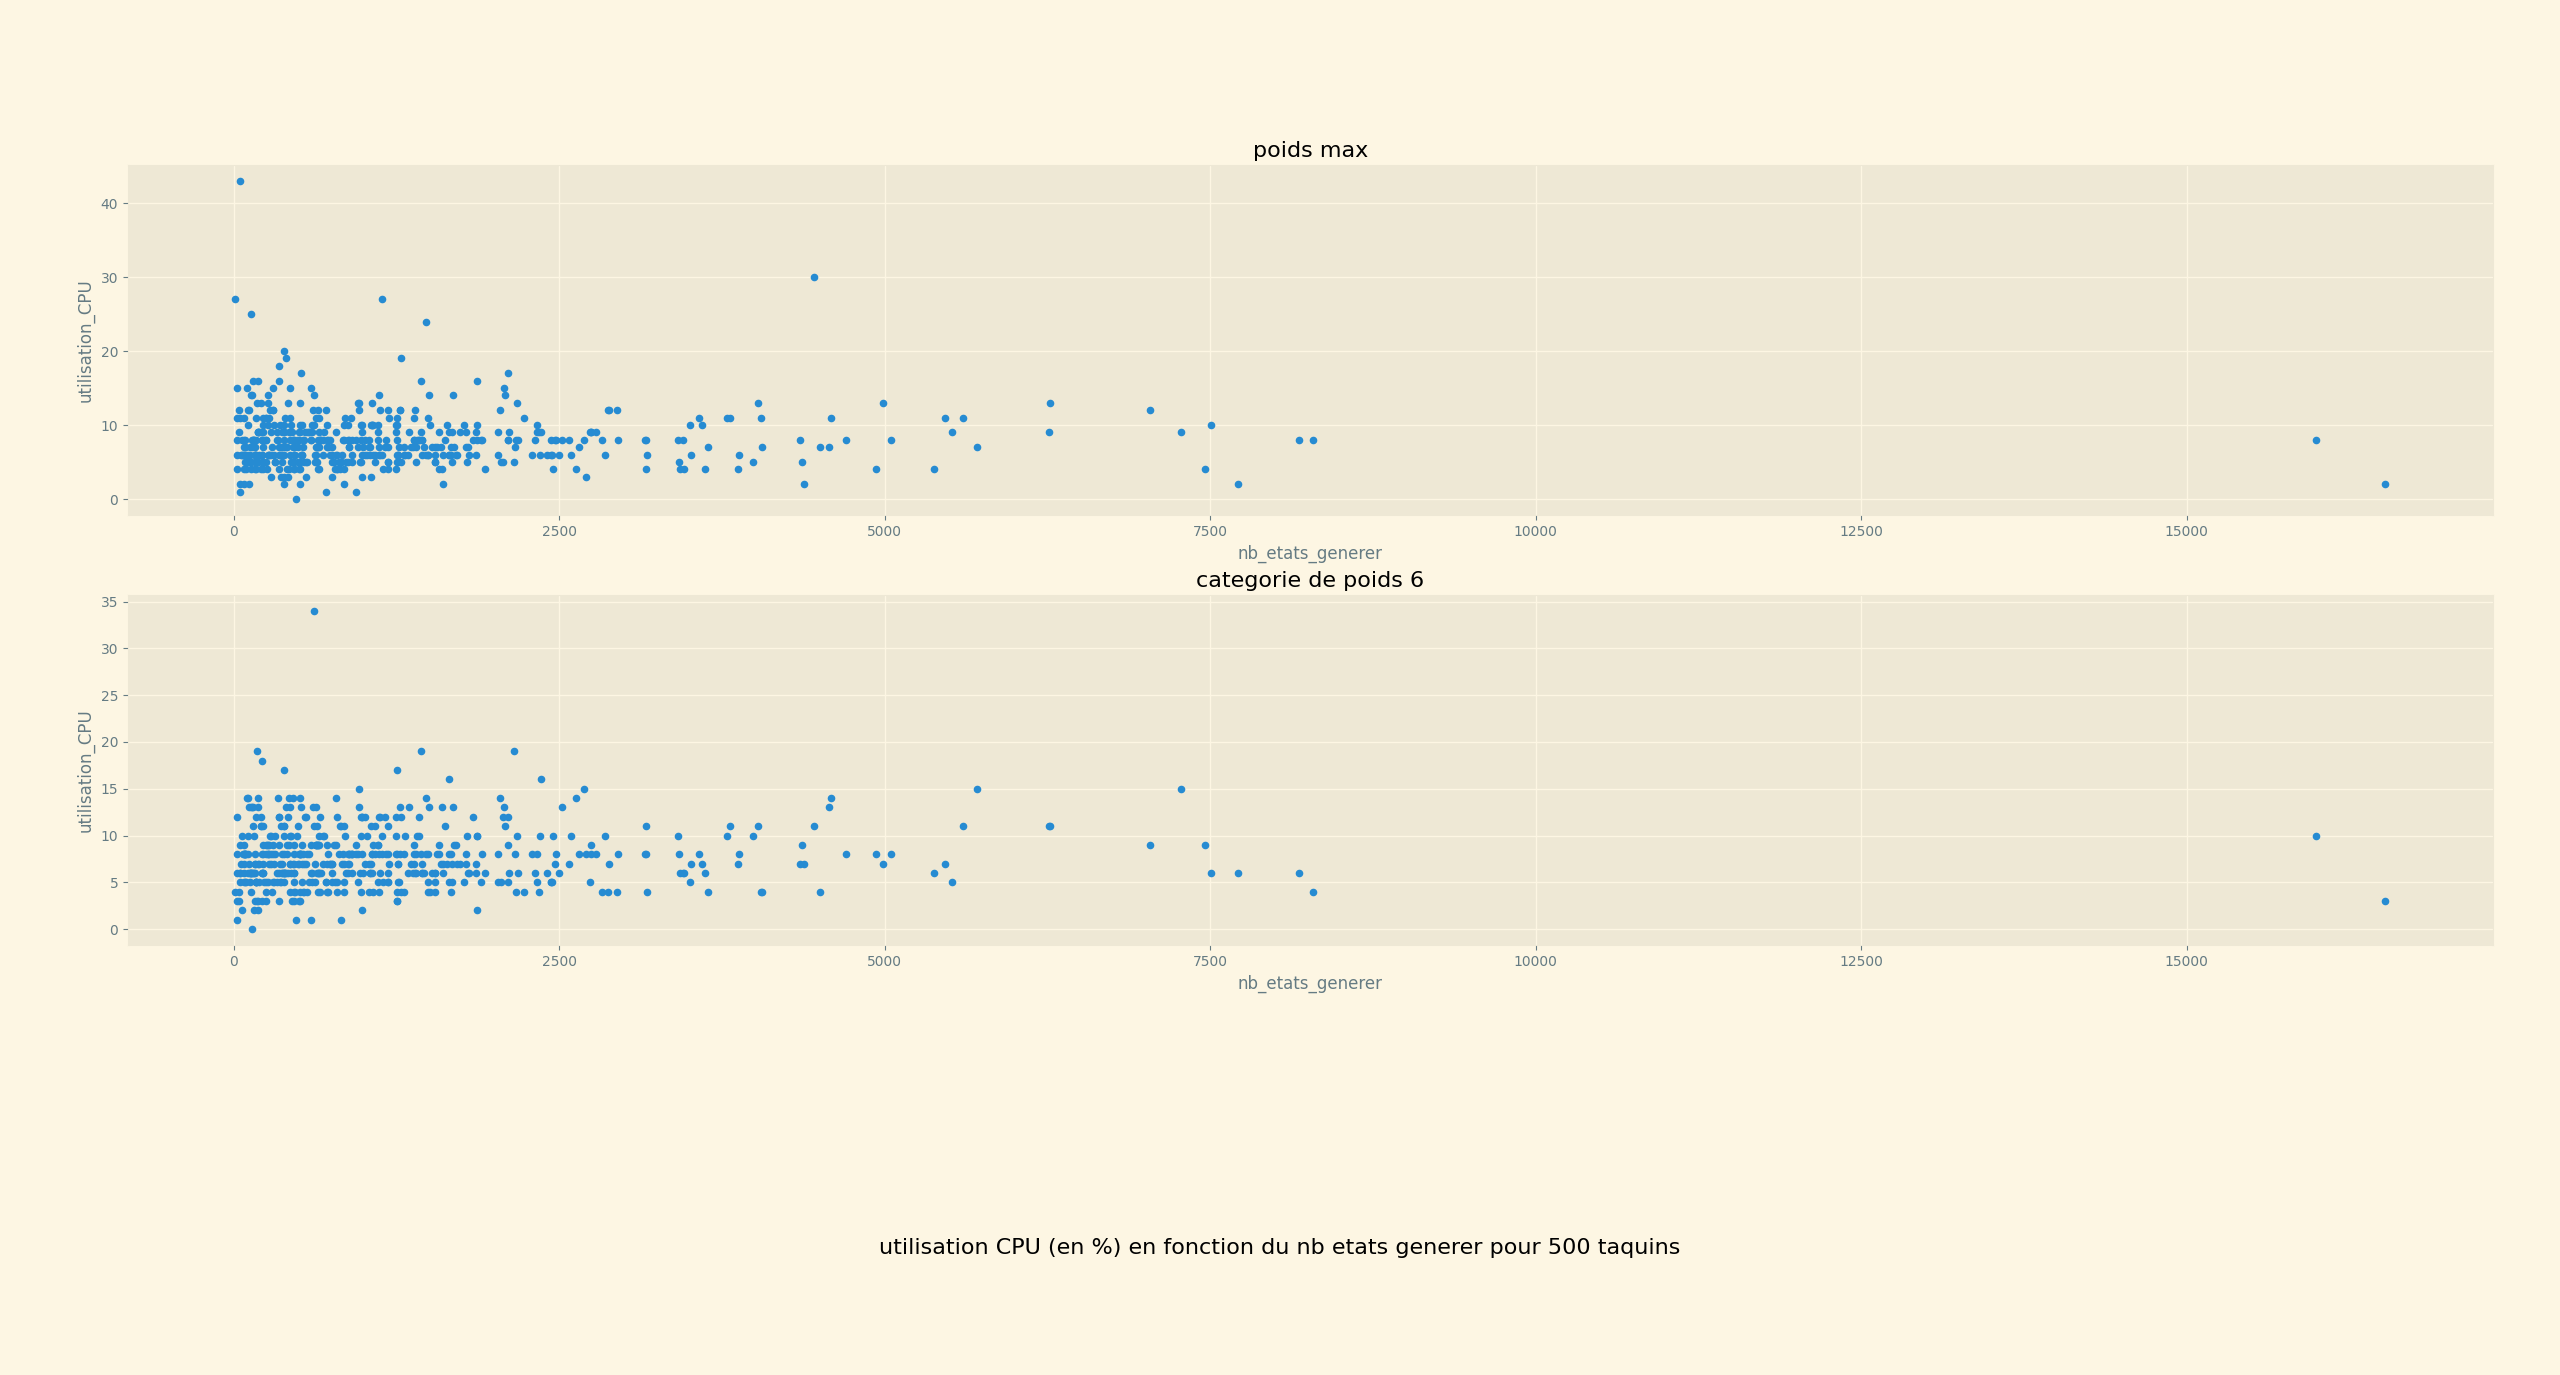
\includegraphics[width=\textwidth]{Taquin 3x3 utilisation CPU en fct du nb d'etat generer}
\end{figure}

\begin{figure}[H]
    \centering
    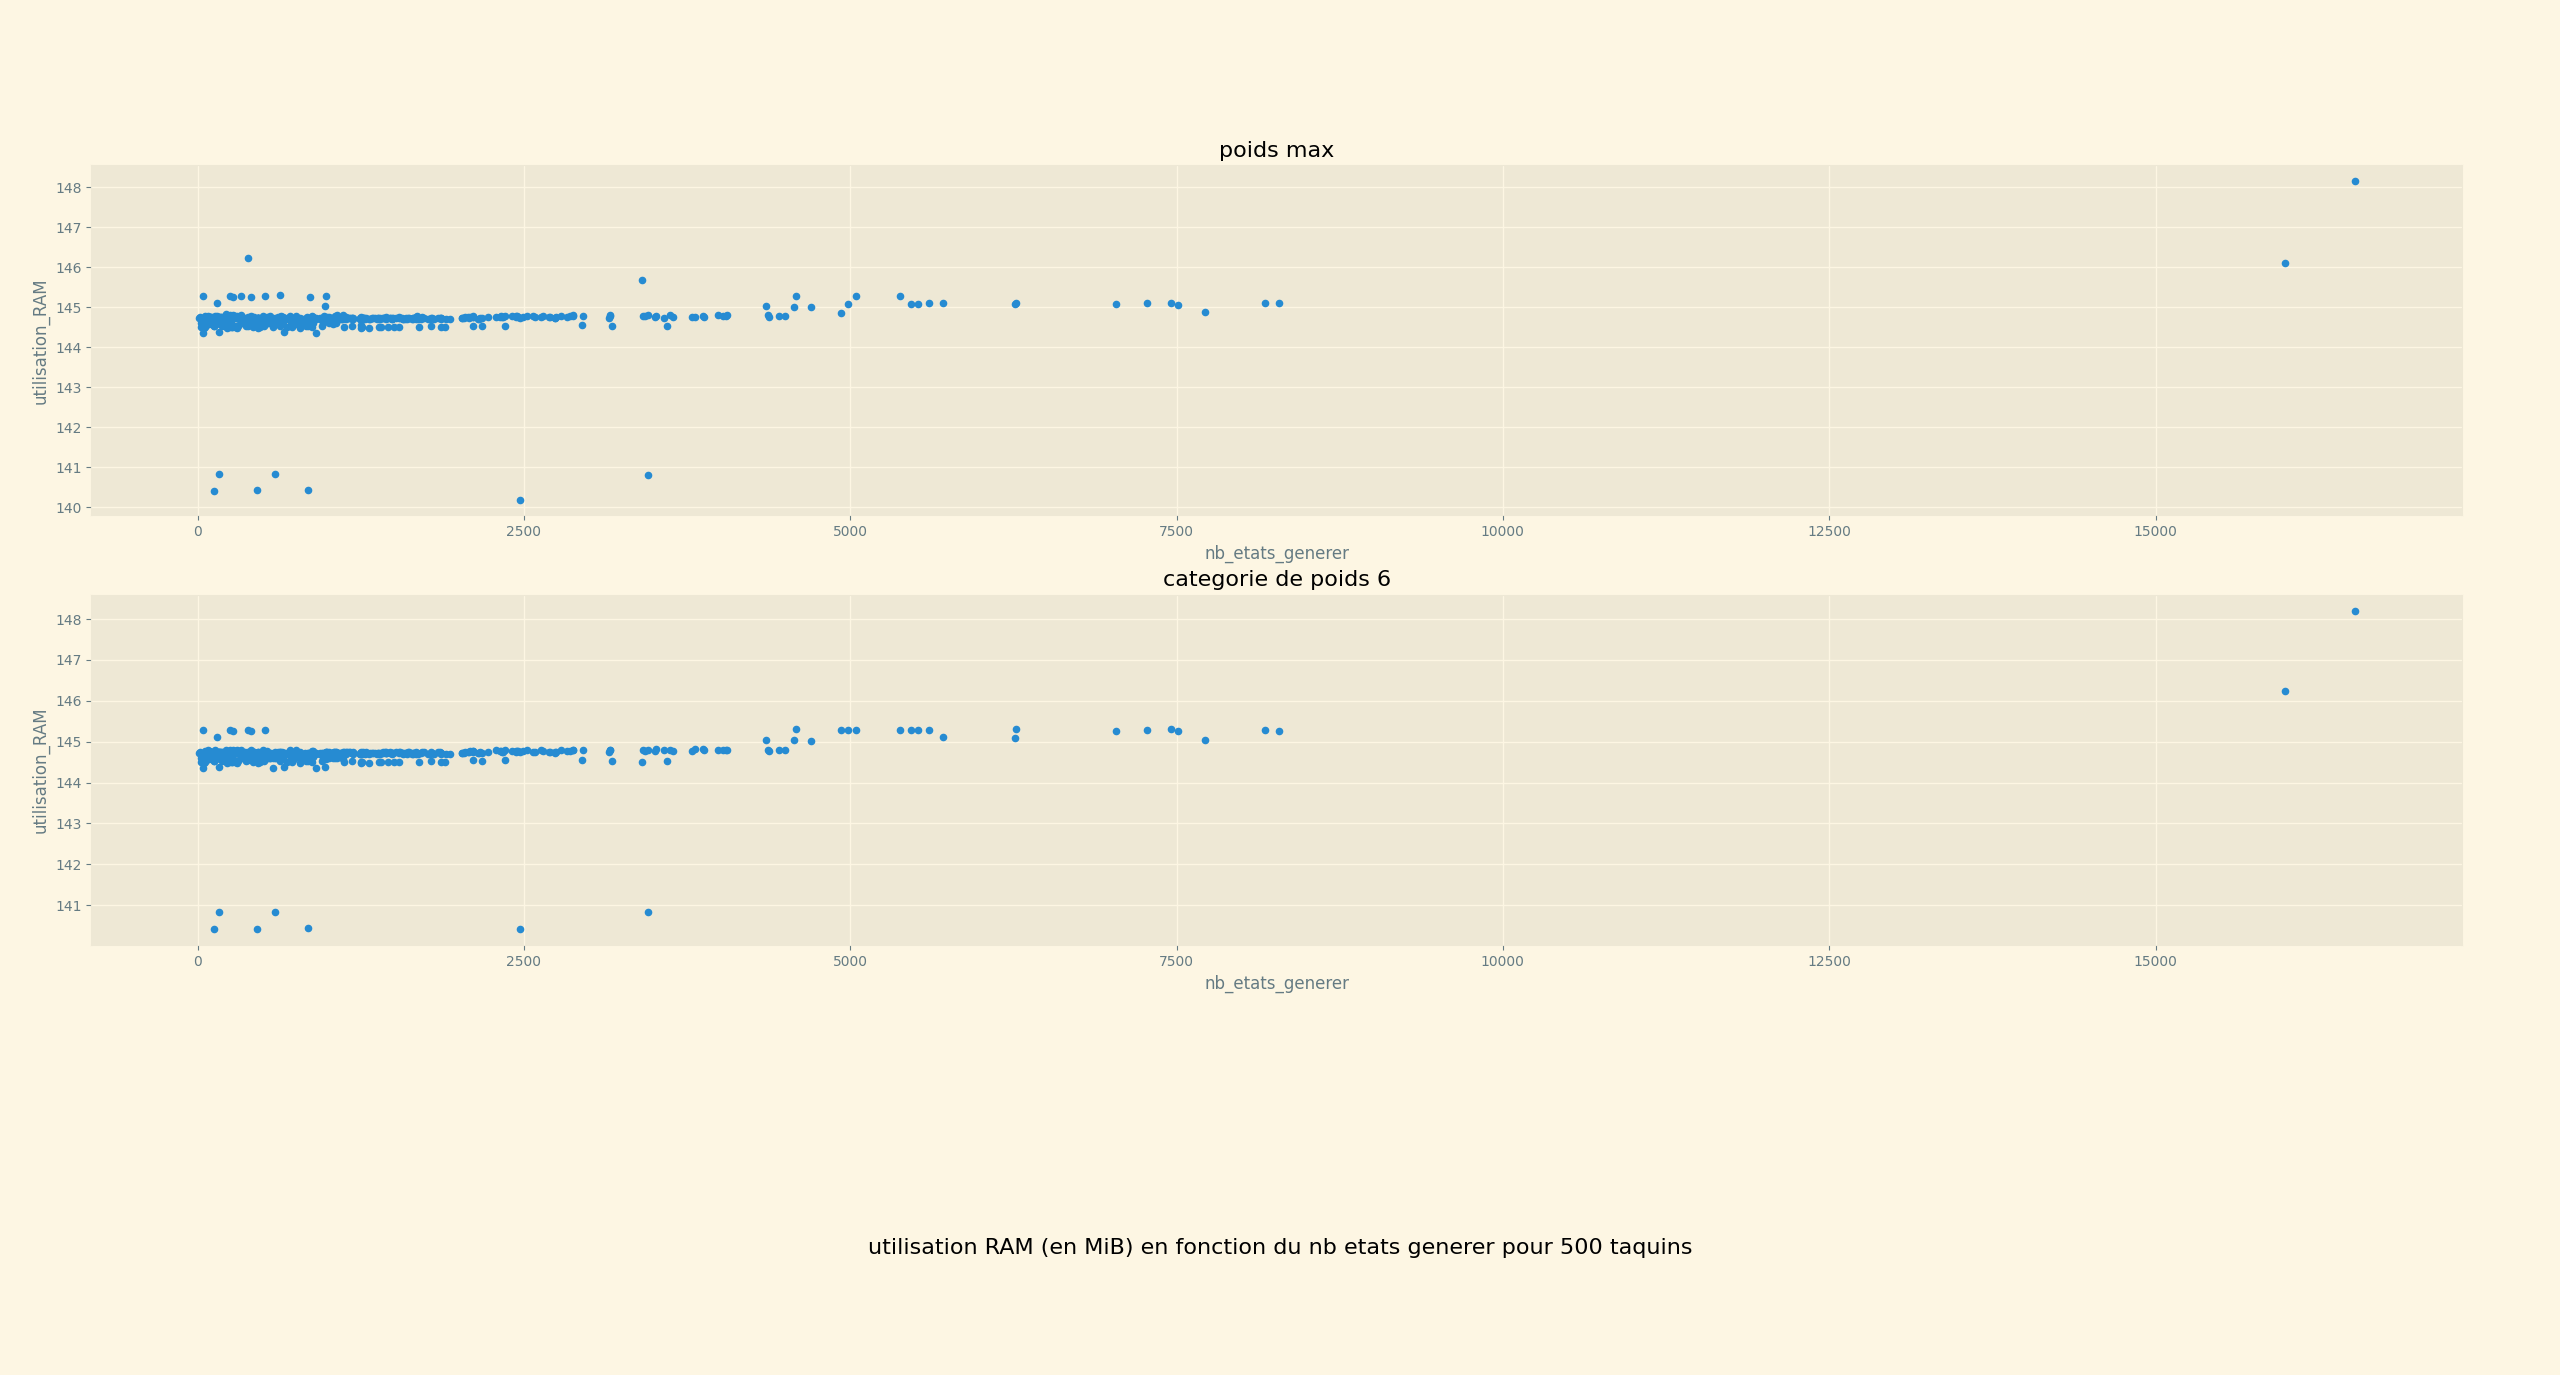
\includegraphics[width=\textwidth]{Taquin 3x3 utilisation RAM en fct du nb d'etat generer}
\end{figure}

\begin{figure}[H]
    \centering
    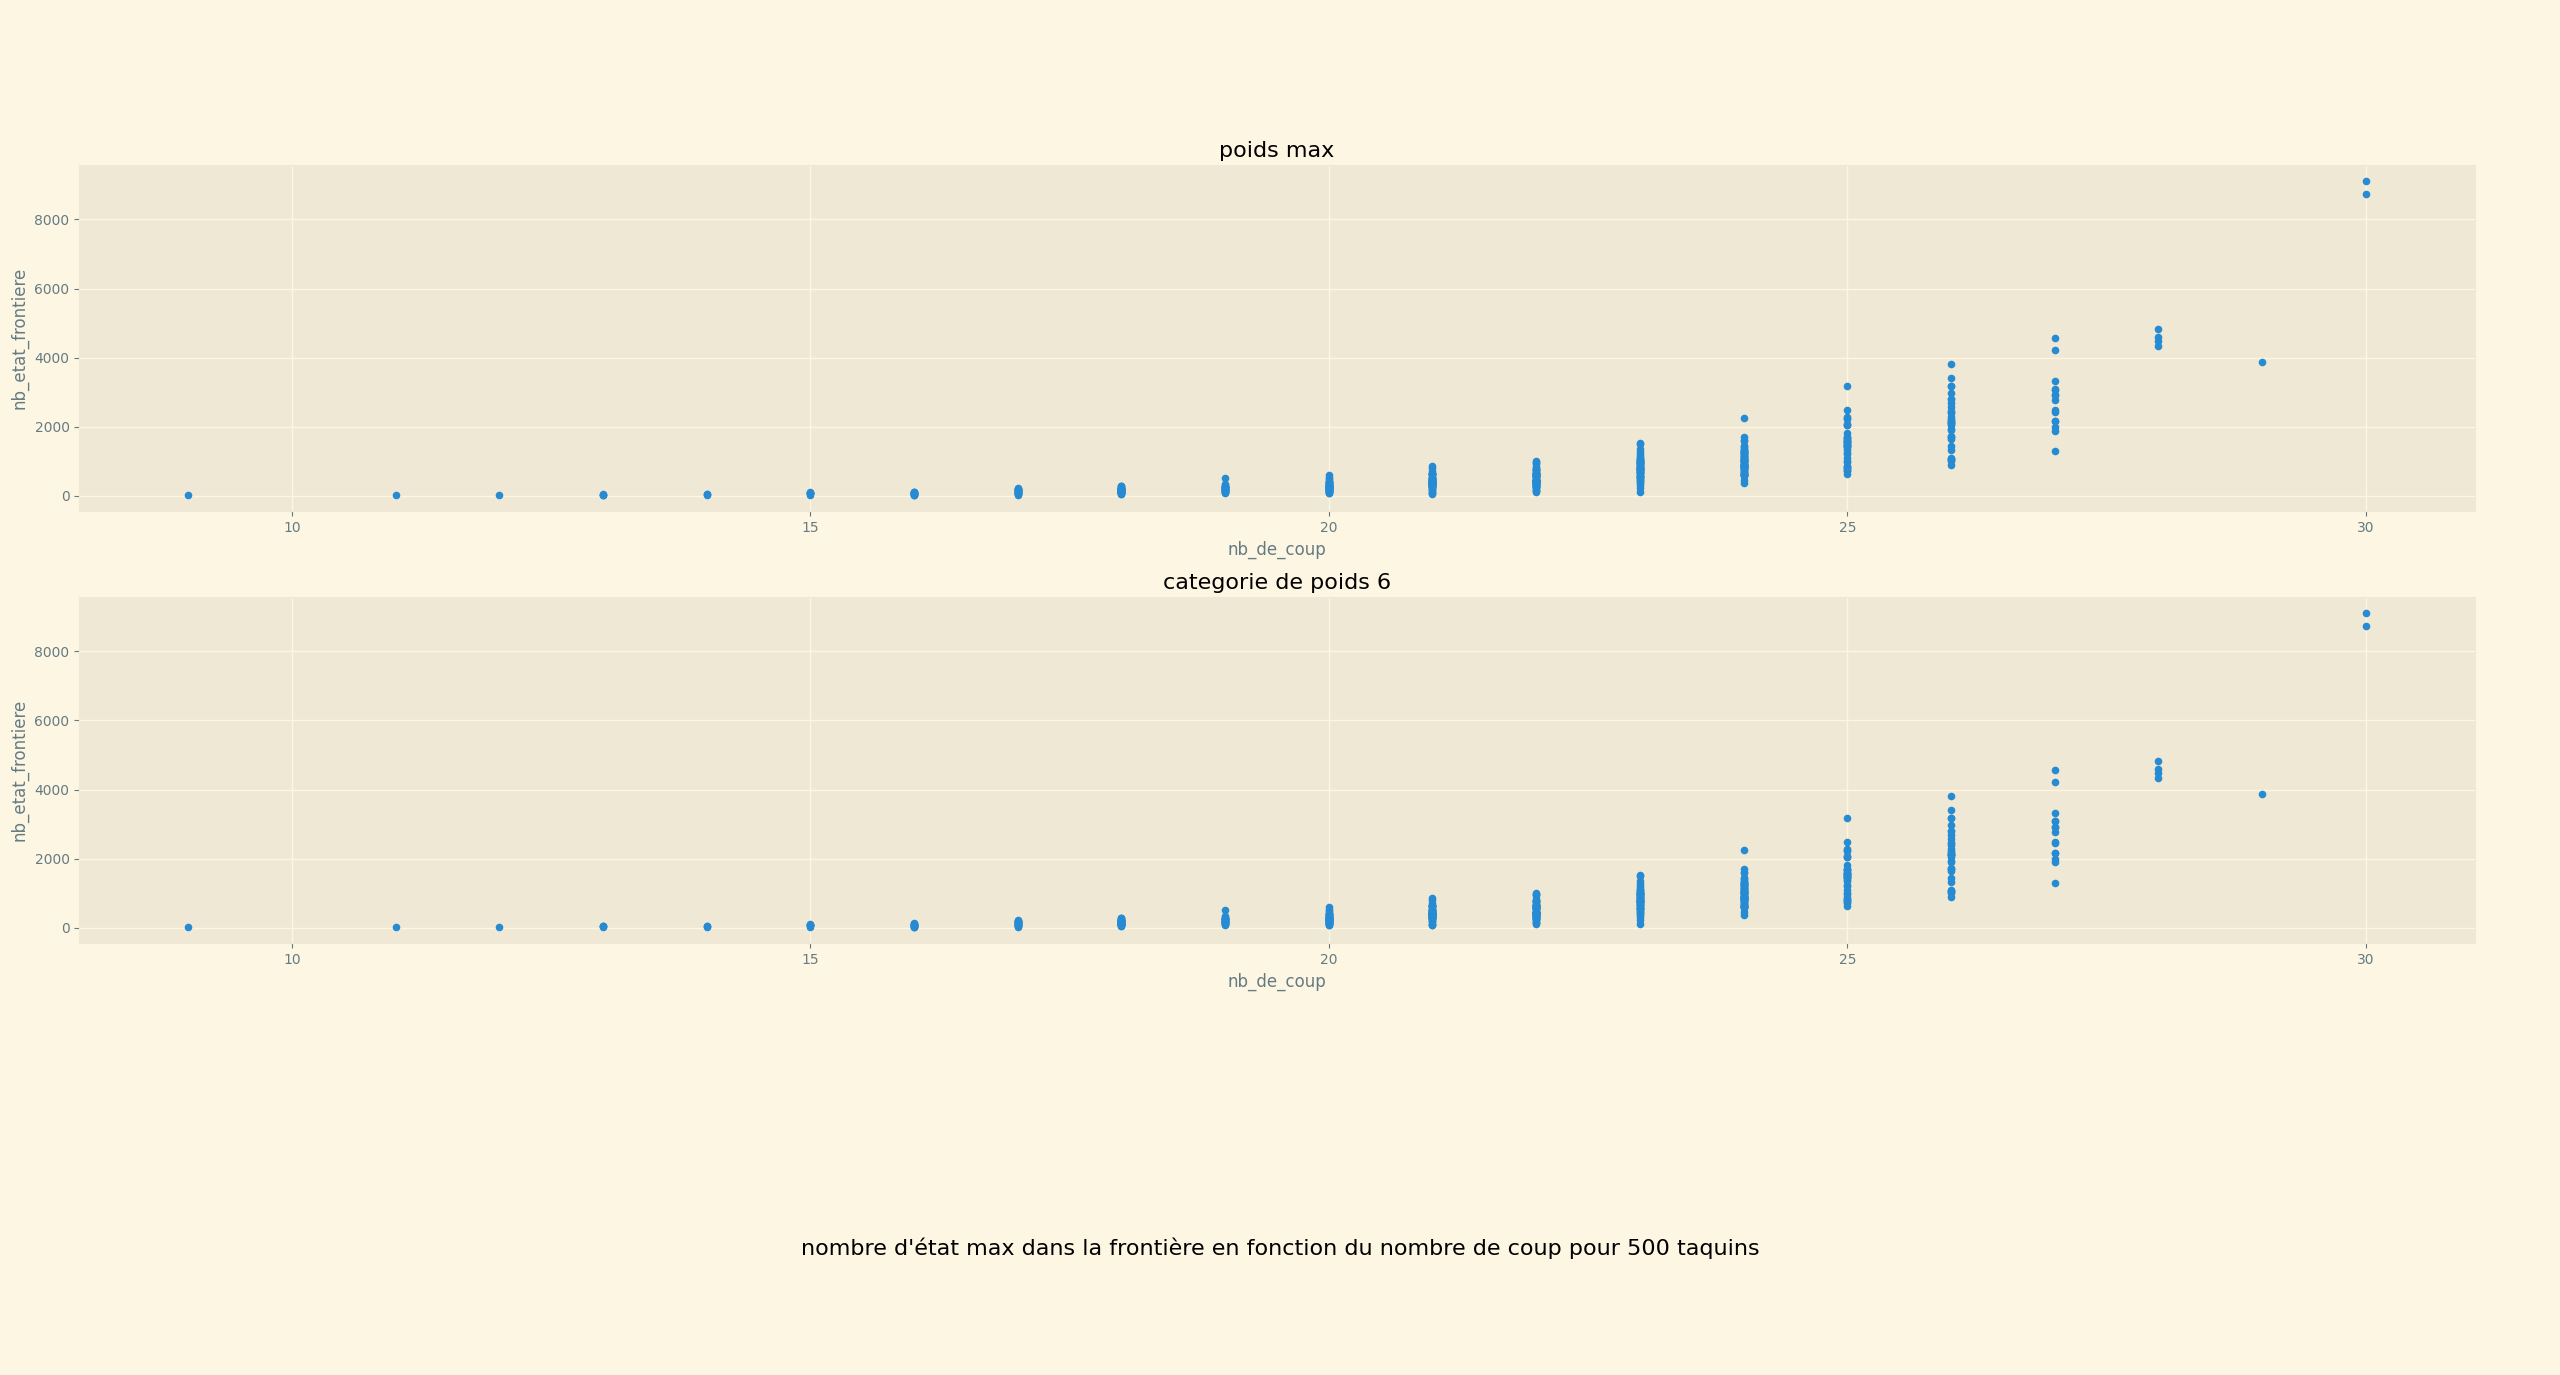
\includegraphics[width=\textwidth]{Taquin 3xnb etat dans la frontiere en fct du nb de coups}
\end{figure}

On observer que les solutions avec une heuristique sans coefficiant de normalisation tend à surrestimer le nombre de coups pour résoudre le taquin.  Le fait de faire le maximum des heuristiques ne change pas le nombr d'état à expanser pour résoudre le taquin 3x3. On peut donc conclure que pour un taquin d ecette taille il est inutile de faire le maximum des heuristiques. Cela n'augmente que le temps de calcul.

\section{Solutions proposées}

\subsection{Algorithme: IDA*}

\subsubsection{Étude de l'algorithme}

IDA* ou Iterative Deepening A* est un algorithme itératif dont l'objectif des itérations est de trouver le prochain mouvement à faire.
Grâce à ça on explore que les états les plus intéressants ce qui réduit drastiquement la complexité en espace : $\mathcal{O}(d)$ où d est la profondeur de la solution.
IDA* a les même propriétés que A*. Il est donc admissible et optimale si l'état final est atteignable depuis l'état initial et que le calcul de l'heuristique respecte aussi les conditions citées plus haut.

\subsubsection{Implémentation}

L'implémentation de IDA* se base sur deux fonctions :
\begin{enumerate}
    \item \lstinline{search} est une fonction récursive qui explore les successeurs d'un état, et si la grille issue de l'un d'entre eux n'est pas dans la liste des grilles déjà rencontrées avant, alors elle appelle à nouveau \lstinline{search} avec cet état.

          Cette fonction prend en paramètre les grilles des états précédemment explorés et conservés, le coût des actions jusqu'alors et une valeur \lstinline{bound}, qui représente une estimation du coût pour résoudre le taquin.

          On sort de \lstinline{search} si on a trouvé l'état final, ou alors si on a exploré tous les états $e$ où $f(e) \leq $ \lstinline{bound}, et on renvoie respectivement -1 ou la valeur minimale du coût estimé dans les états restants.

    \item La fonction \lstinline{ida_star}, quant à elle, calcule l'heuristique de l'état initial, et appelle \lstinline{search} avec \lstinline{bound} comme étant une estimation du coût de la solution optimale, celle-ci étant renvoyée par \lstinline{search}.

          Si \lstinline{search} trouve une solution, \lstinline{ida_star} renvoie la liste des états parcourus pour trouver la solution, sinon -1 si \lstinline{search} renvoie $\infty$.
\end{enumerate}

\subsubsection{Inconvénients}

\subsection{Heuristique : conflit linéaire}


\subsubsection{Étude de l'heuristique}

Le principe de l'heuristique du conflit linéaire est le suivant: 2 tuiles 'a' et 'b' sont en conflit linéaire si elles sont dans la même ligne ou la même colonne, que leur position finale est aussi dans la même ligne ou colonne et qu'au moins l'une des tuile est bloquée par la seconde pour arriver à sa position finale sans considérer la case vide.
Le calcul de cette heuristique sera égale à $2 \times nblc + Md$, où $nblc$ est égal au nombre de conflits linéaires sur chaque ligne + le nombre de conflits linéaires sur chaque colonne, et Md est la distance de Manhattan. Cette fonction est donc une faible amélioration de la distance de Manhattan. De plus, on doit utiliser un poids de 1 pour chaque tuile pour ne pas surestimer le coût pour atteindre l'état final.

\subsubsection{Implémentation}

Pour calculer les conflits linéaires, nous avons réalisé 3 fonctions : une fonction principale pour calculer l'heuristique finale, une pour calculer le conflit linéaire pour les lignes et une pour les colonnes. Pour cela si on a un taquin de taille $n \times n$, on devra donc faire $2 \times (n^2*(n-1))$ opérations pour calculer les conflits linéaires (sans prendre en compte le calcul de la distance de Manhattan).
On a donc dans le pire cas une complexité en temps de $ \mathcal{O}(n^3)$. Pour calculer le conflit linéaire.

\subsubsection{Inconvénients}

Même si celle ci améliore l'estimation du coût de la solution, elle augmente le temps de calcul du programme pour des taquins de grande taille.
En explorant quelques centaines de milliers d'états par seconde, il serait possible de résoudre des taquins 4x4 mais pas au dessus.

\subsection{Amélioration possible de l'heuristique}
Il est possible d'améliorer la complexité temporelle de ce programme en réalisant quelques modifications. On peut remarquer que déplacer une tuile le long d'une ligne ne résout aucun conflit linéaire sur la ligne (de même sur la colonne). En conséquence, on peut réduire les vérifications uniquement aux lignes et colonnes affectées et donc passer de $\mathcal{O}(n^{3})$ à $\mathcal{O}(n^{2})$.
On peut aussi combiner d'autre heuristiques avec celle de la distance de Manhattan comme "Corner Tile Heuristic" ou encore "Last Tile Heuristic",... Nous ne les développerons toutefois pas ici.

\subsection{Expérimentation}
\begin{figure}[H]
    \centering
    \includegraphics[width=\textwidth]{Taquin 3x3 nombre d'état dans la frontiereen fct du nb du nb de coups linear conflict}
\end{figure}
\begin{figure}[H]
    \centering
    \includegraphics[width=\textwidth]{Taquin 3x3 nombre d'état explorer en fct du nb de coups linear conflict}
\end{figure}
\begin{figure}[H]
    \centering
    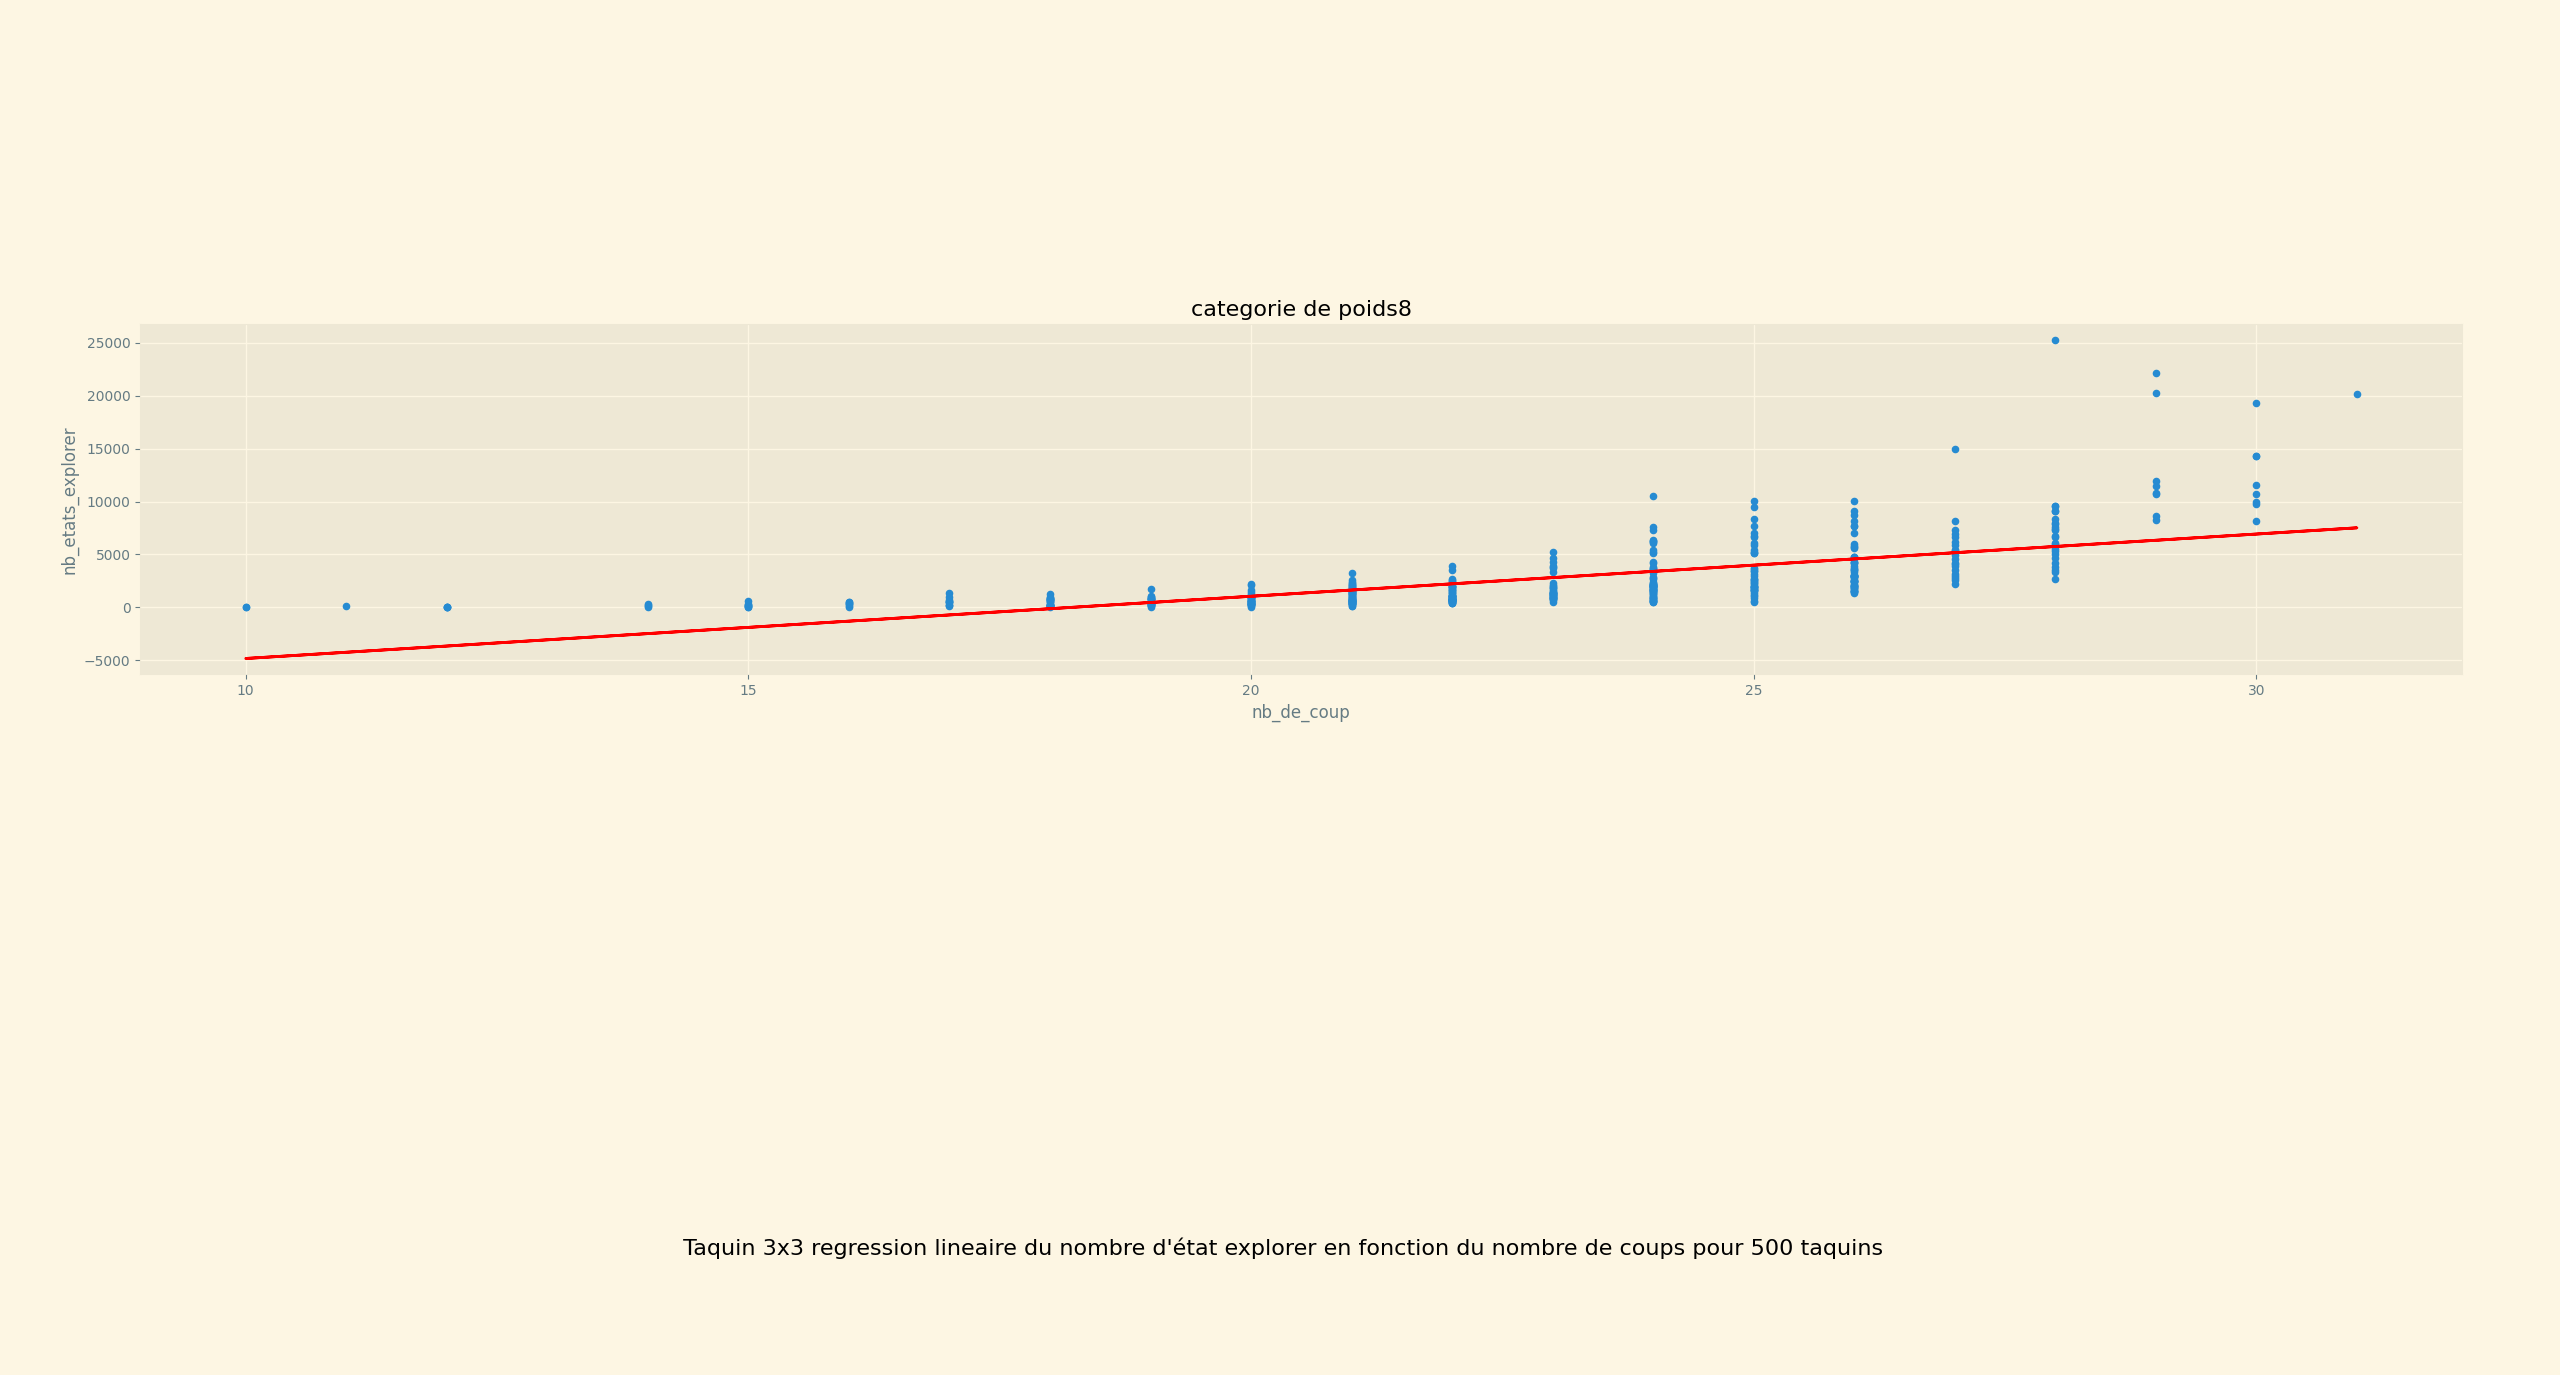
\includegraphics[width=\textwidth]{Taquin 3x3 nombre d'etat explorer en fct du nb de coups reg lineaire Linear conflict}
\end{figure}
\begin{figure}[H]
    \centering
    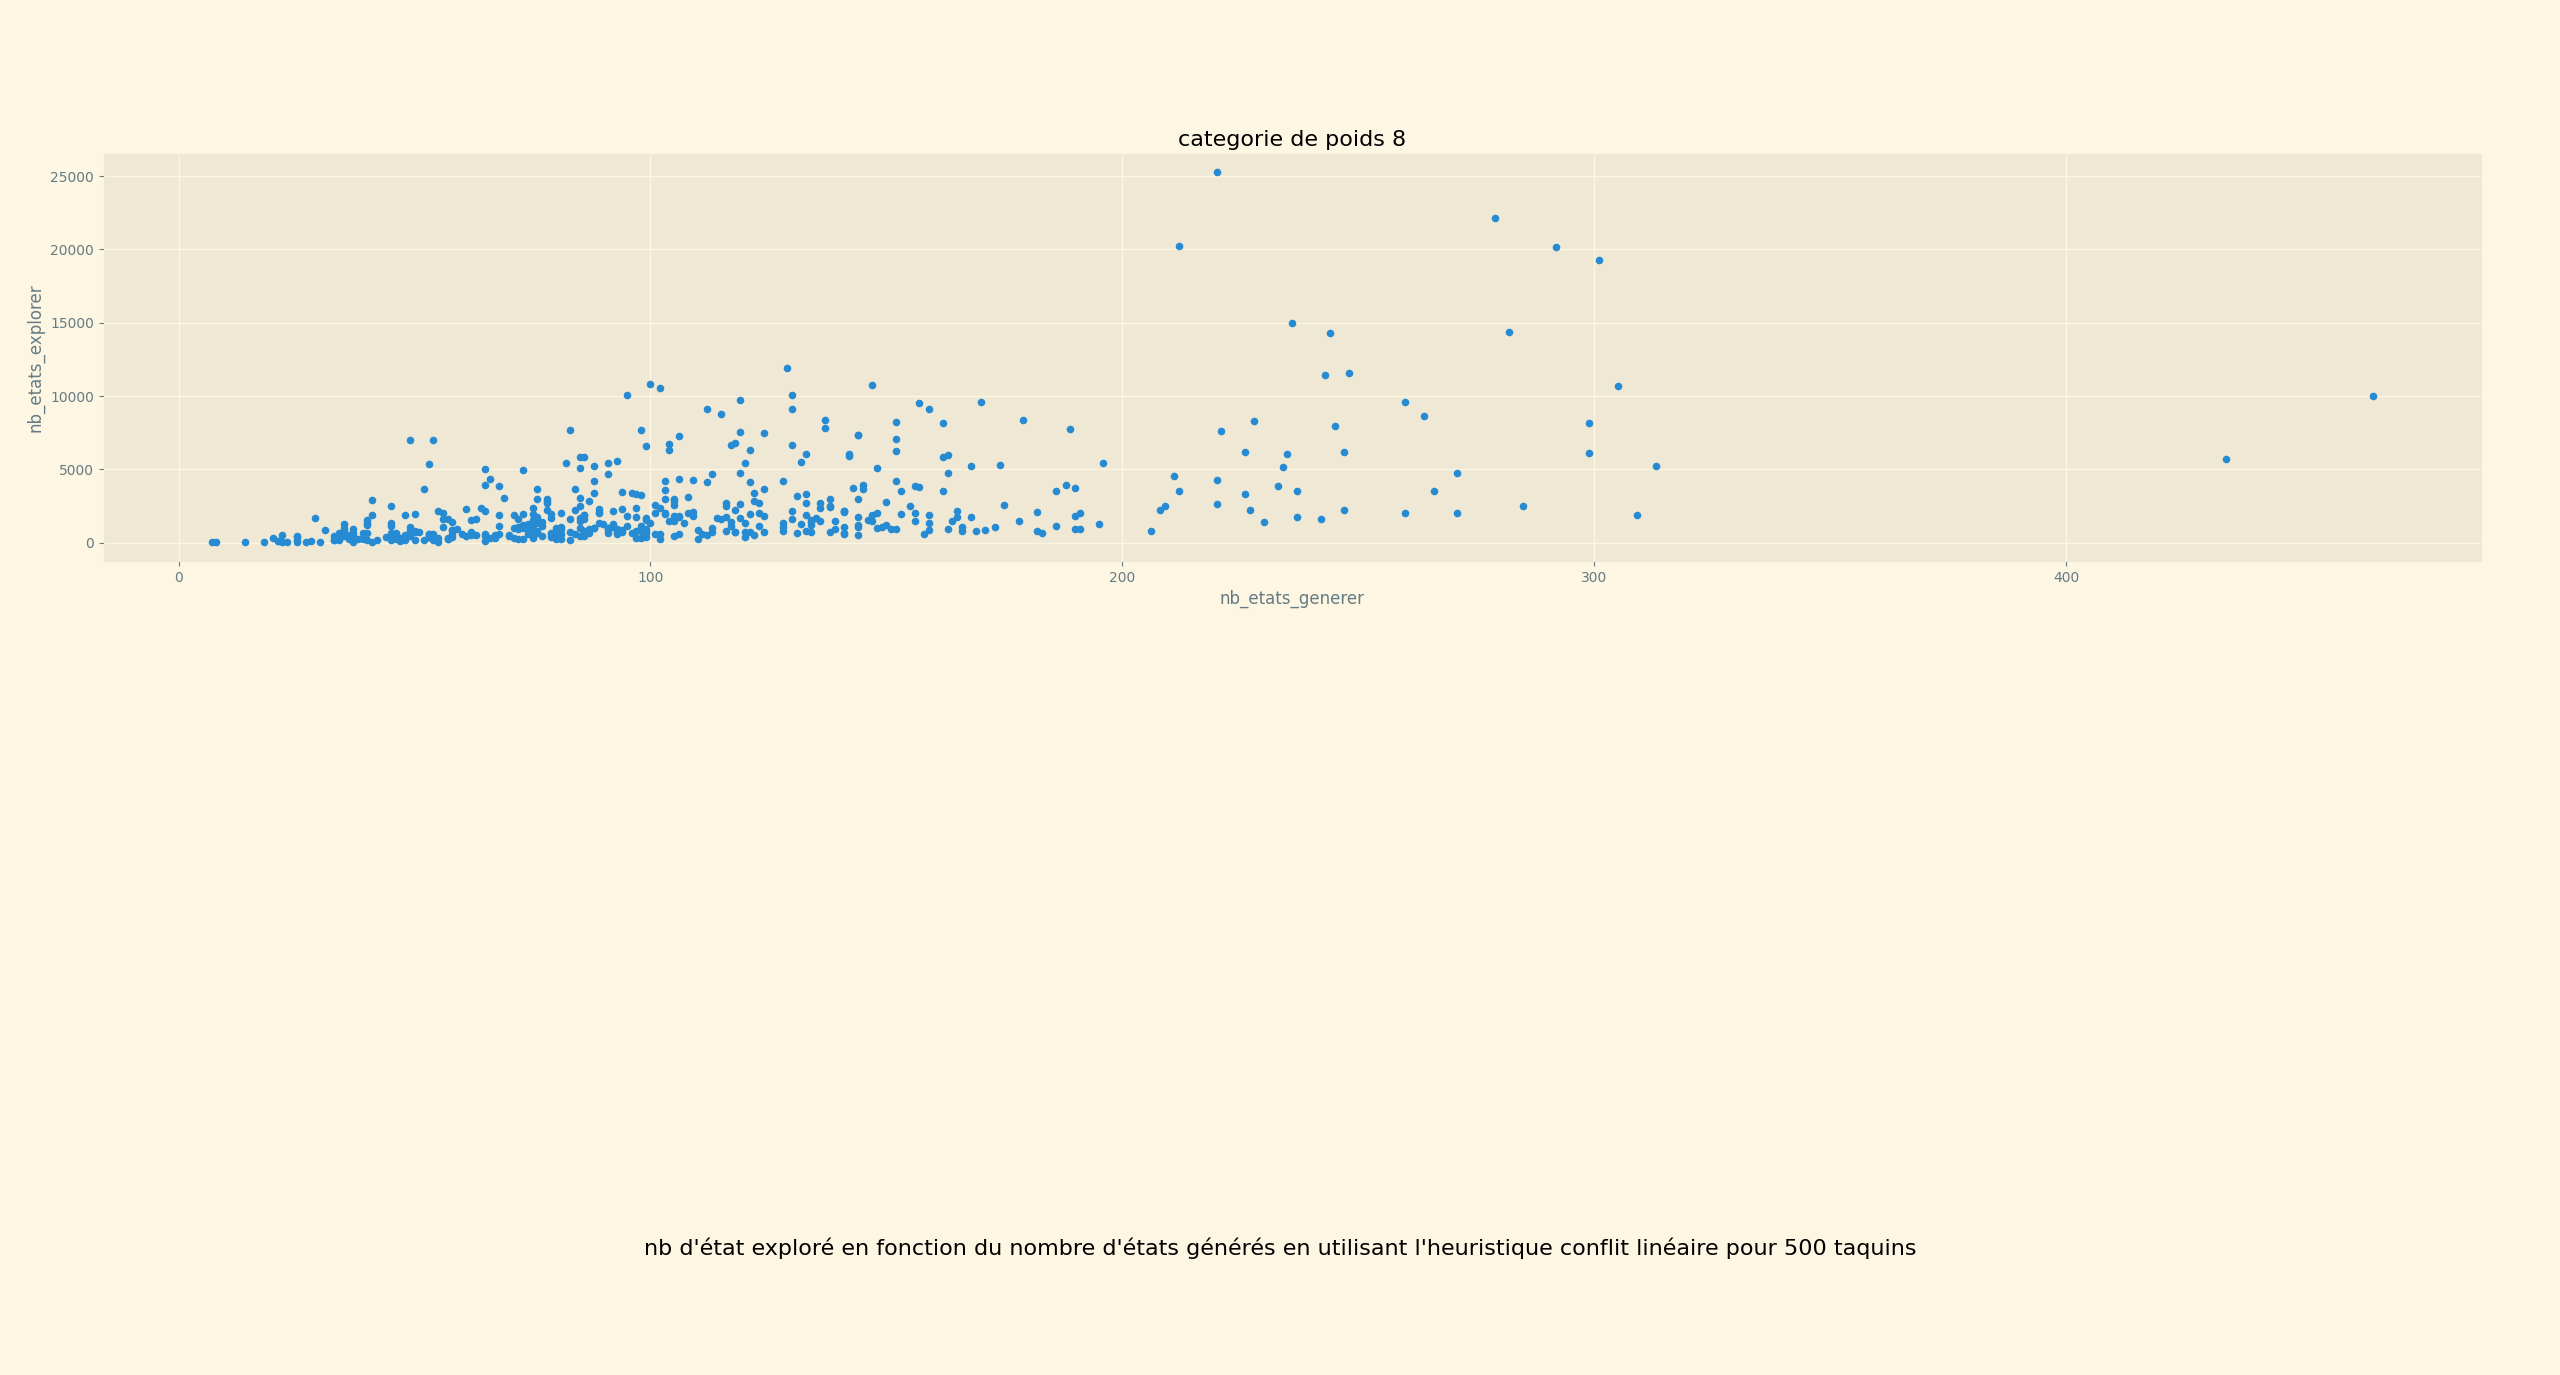
\includegraphics[width=\textwidth]{Taquin 3x3 nombre d'etat explorer en fct du nb de detat generer linear conflict}
\end{figure}
\begin{figure}[H]
    \centering
    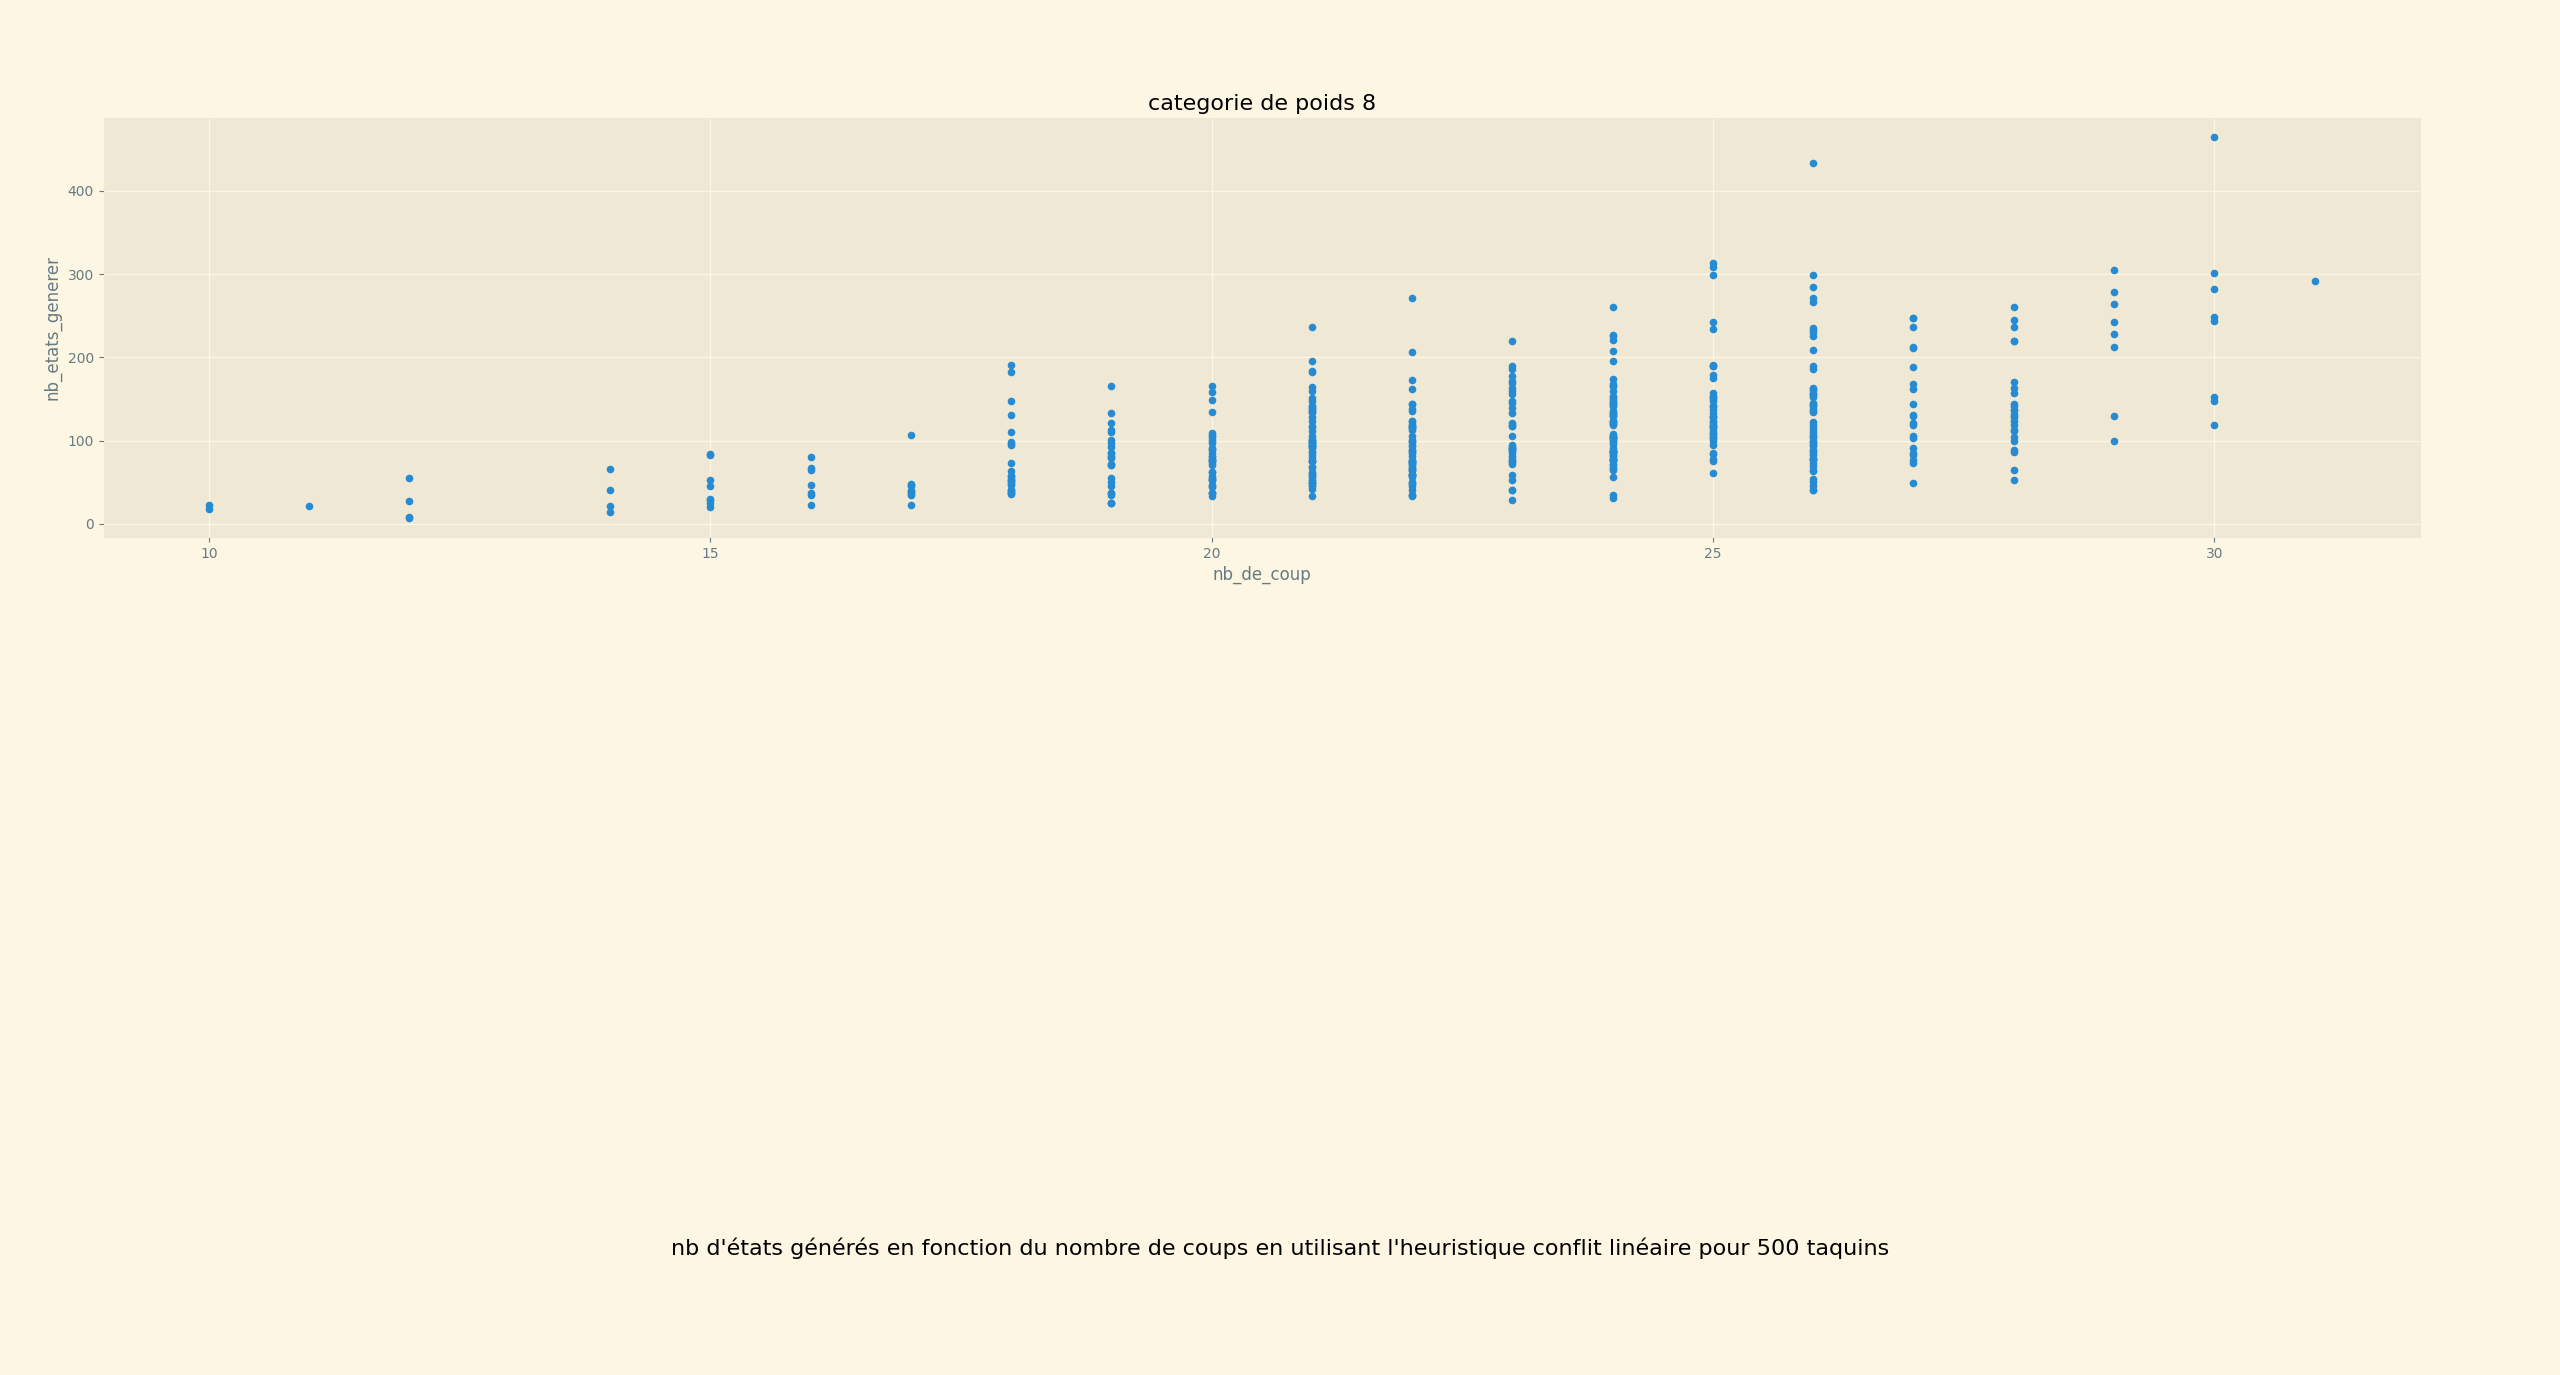
\includegraphics[width=\textwidth]{Taquin 3x3 nombre d'etats generer en fct du nb de coups linear conflict}
\end{figure}
\begin{figure}[H]
    \centering
    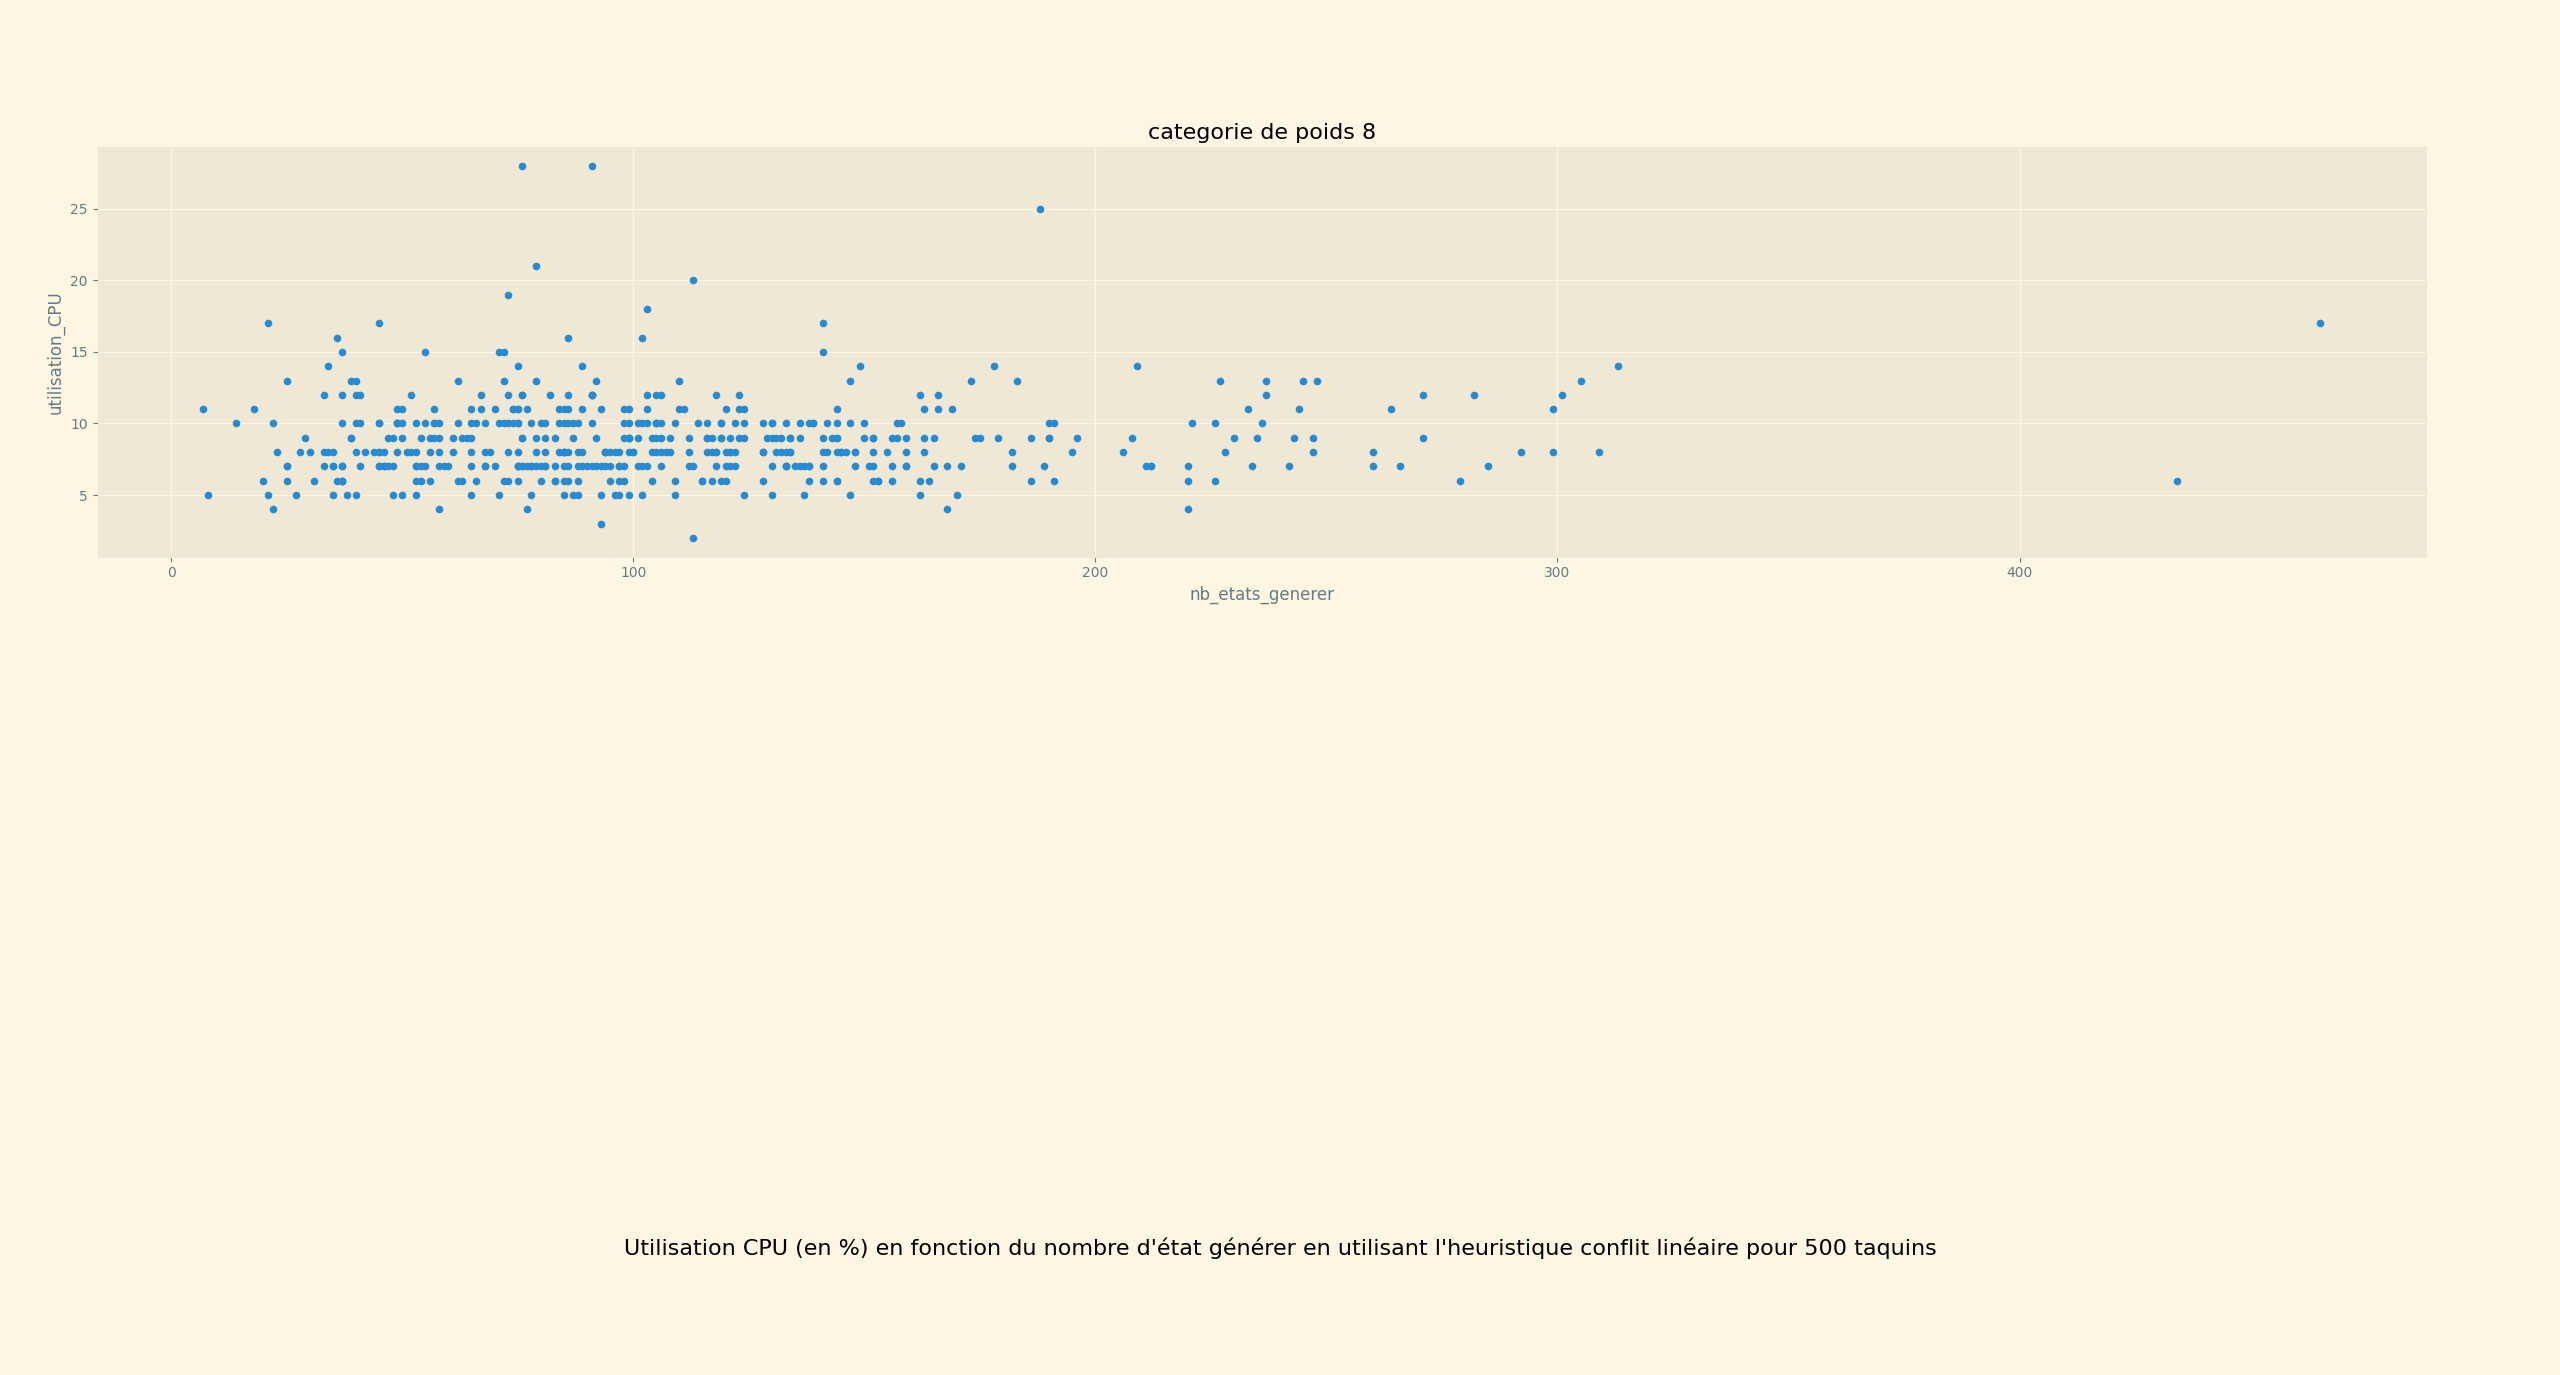
\includegraphics[width=\textwidth]{Taquin 3x3 utilisation CPU en fct du nb d'etat generer linear conflict}
\end{figure}
\begin{figure}[H]
    \centering
    \includegraphics[width=\textwidth]{Taquin 3x3 nombre d'état explorer en fct du nb detat ds la frontiere linear conflict}
\end{figure}

\begin{figure}[H]
    \centering
    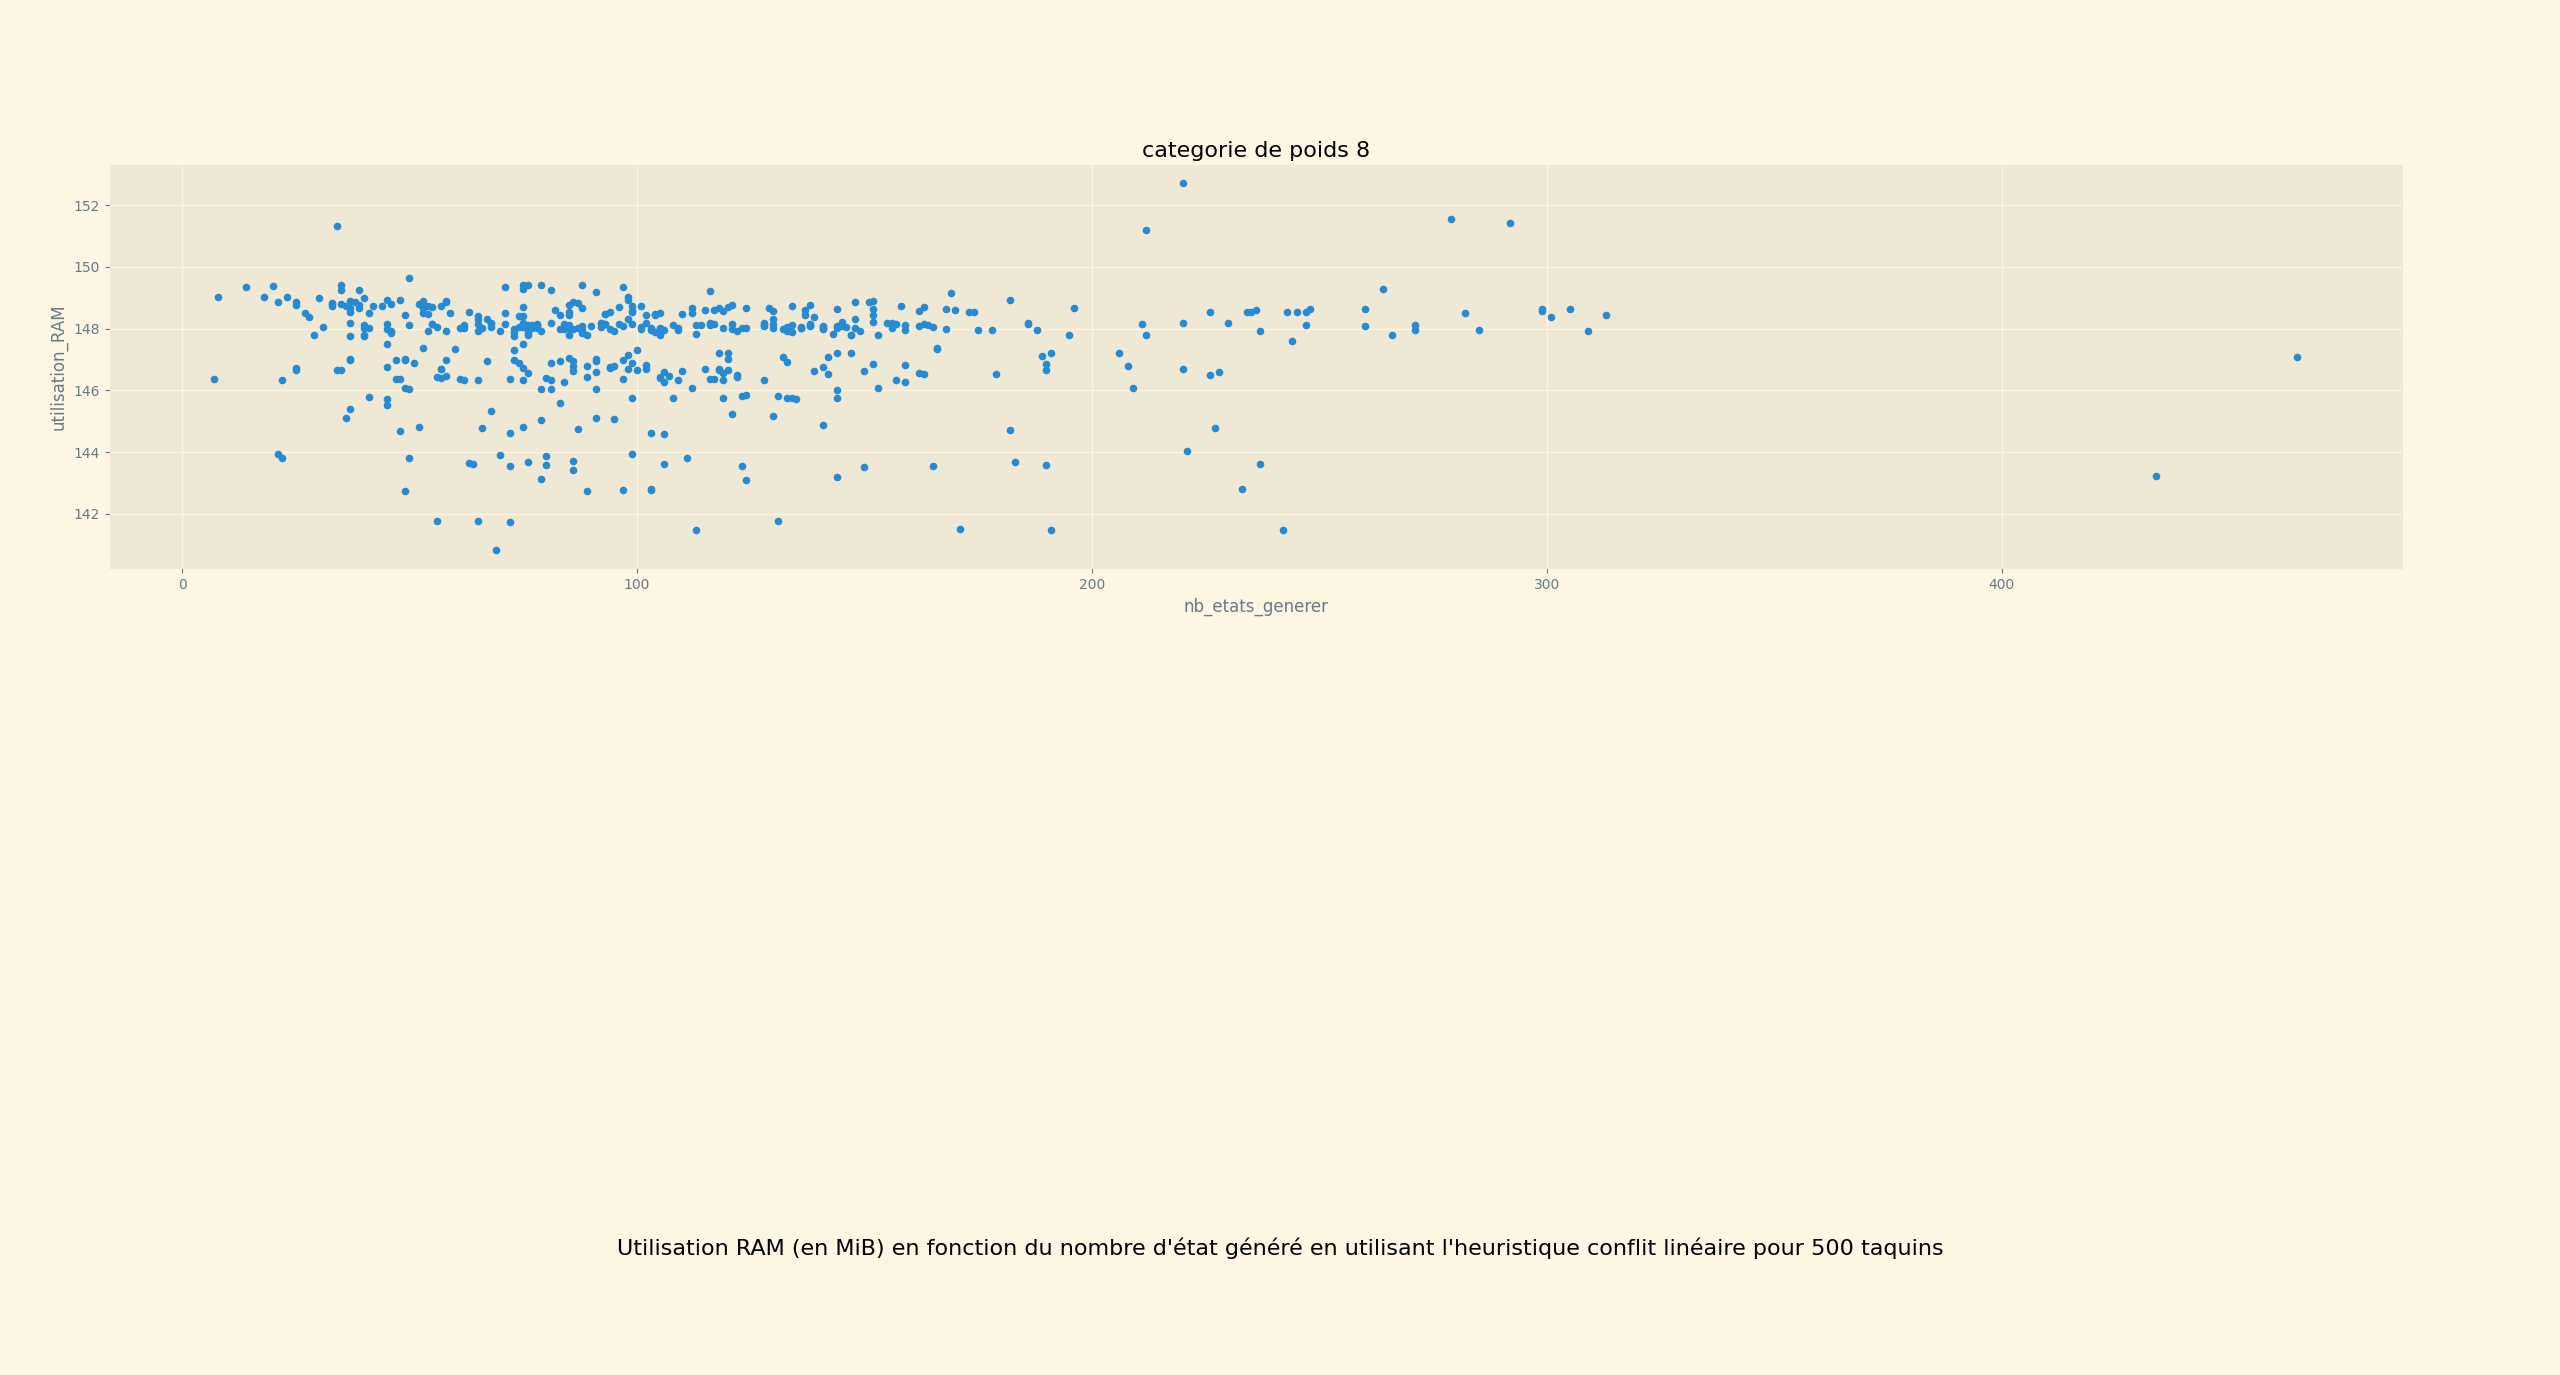
\includegraphics[width=\textwidth]{Taquin 3x3 utilisation RAM en fct du nb d'etat generer conlit lineaire}
\end{figure}

On peut observe que linear conflict ne fait qu'augmenter le temps de calcul pour les taquins de taille $3 \times 3$.
\subsection{Heuristique : Walking distance}

\subsubsection{Étude de l'heuristique}

L'heuristique Walking Distance a été créée dans les années 2000 par le programmeur Ken'ichiro Takahashi, alias takaken.

Le principe de la walking distance est d'attribuer à chaque case une lettre correspondant à sa ligne finale (A pour la 1ère, B pour la 2e, ...), de placer les cases d'une même ligne dans une "boîte", et de calculer combien de mouvements d'une case d'une boîte à une autre boîte adjacente faut-il faire pour que chaque boîte ne contienne que les cases qui correspondent à sa ligne (les A dans la boîte 1, les B dans la boîte 2, ...).
On fait de même sur les colonnes et on fait la somme avec le résultat sur les lignes, et on obtient finalement la valeur de la walking distance pour une grille qui correspondrait à ce schéma.

On stocke le résultat pour chaque schéma dans une base de données, et ensuite pour utiliser effectivement l'heuristique, on calcule le schéma de la grille actuelle et on cherche dans la base données à quelle walking distance elle correspond.

Dans le cas des grilles $4 \times 4$, on a 24964 schémas à générer, ce qui est raisonnable d'un point de vue espace et temps.

Cette heuristique est admissible.

\subsubsection{Implémentation}

Pour la partie génération des walking distances, on part de la grille finale avec les cases aux bonnes positions, et on avance dans l'arbre des grilles en déplaçant une case à chaque fois.

Pour chaque grille, on calcule la matrice correspondant aux positions des cases sur la grille par rapport à leur position finale, donc dans le cas d'une grille $4 \times 4$, on a une liste $4 \times 4$ où les cases $(i, j)$ correspondent au nombre de cases, dont la ligne ou colonne finale est i, qui sont sur la ligne ou colonne j.
On attribue ensuite au schéma des lignes ou colonnes un identifiant de la grille en utilisant des opérations bit par bit.
On stocke les identifiants des schémas et leur valeur de walking distance dans une base de données sqlite.

Ensuite, on charge cette base de données dans un dictionnaire, pour que les valeurs soient rapidement accessibles, et quand on calcule la walking distance d'une grille, on fait la somme de la walking distance sur le schéma des lignes et sur le schéma des colonnes.

\subsubsection{Avantages}

Cette méthode de calcul d'heuristique estime bien mieux le véritable coût que la distance de Manhattan, car elle prend en compte la position de la case vide. Aussi, le gros du calcul est fait en amont dans la base de données, celle-ci prenant quelques secondes à se générer, et celle-ci a une taille extrêmement raisonnable, seulement 1.6Mo avec notre implémentation, donc elle est aussi très rapide à charger.

Ainsi, il suffit juste de chercher dans le dictionnaire des walking distances l'identifiant qu'on a calculé pour les lignes et pour les colonnes.
La recherche dans un dictionnaire étant très rapide, on peut calculer de manière efficace la walking distance tout en ayant une meilleure précision qu'avec la distance de Manhattan.

\subsubsection{Inconvénients}

Malgré sa meilleure efficacité, cette méthode nécessite tout de calculer énormément d'états, et donc pour les grilles les plus difficiles le calcul de la solution reste très long.
Il existe des solutions pour optimiser au maximum la résolution avec walking distance, mais elles sont assez complexes et difficiles à mettre en place dans le cadre de ce projet.

\subsubsection{Améliorations possibles}

Il existe plusieurs programmes trouvables sur Internet, notamment un par le créateur de cette heuristique, qui résolvent un taquin complexe en quelques secondes avec Walking Distance, mais nous n'avons pas réussi à atteindre leur niveau de performances.

Il serait possible de combiner la walking distance avec d'autres heuristiques pour estimer encore mieux le coût, mais nous n'avons pas pu mettre ça en place d'une bonne manière.

\subsection{Heuristique : Pattern Databases (additif)}


\subsubsection{Étude de l'heuristique}

Inventé par Culberson et Schaeffer (1994), son principe est d'utiliser un base de données à l'aide de patterns et de pouvoir générer une heuristique quasi parfaite. Elle est garantie d'être consistante, d'être inférieure au coût de la solution du plus court chemin et plus le pattern est grand mieux c'est. Des taquins de taille supérieure à $3 \times 3$ ayant beaucoup trop d'états pour être stockés entièrement ou même générés, nous allons générer plusieurs patterns pour diminuer le nombre d'états à stocker dans la mémoire.
Pour un taquin de taille $N = n \times n$, le nombre d'états à stocker ne sera plus que de $\frac{N!}{(N-t)!}$ (où t est le nombre de tuiles dans le pattern), comme on plus que t tuiles à considérer. Grâce à ça, on pourra avoir une heuristique très proche de la réalité comme le coût prendra maintenant en compte le déplacement de la case avec la case vide pour arriver de son état actuel à sa position finale.
Enfin pour faire cela on part de l'état final pour générer toutes les dispositions possibles.
Il existe plusieurs types de patterns databases comme par exemple celle que nous avons décidé d'utiliser qui est dite \lstinline{Static Additive Pattern Database} ou \lstinline{Dynamically partitioned Additive Pattern Database} qui prend en compte la valeur de la parité des distance et la distance de Manhattan (il peut aussi être utilisé pair+triple+quadruple). Ceci a pour avantage de rendre la génération de la base de données plus rapide et bien moins lourde.
En contre partie, celle-ci prendra plus de temps pour résoudre les taquins car stockant moins de cas. Dans notre cas, on utilise une base de données static. Il existe aussi des heuristiques qui n'utilisent qu'un seul pattern pour calculer celle-ci.
Pour cela nous allons générer des patterns tels que toutes valeurs en dehors d'un pattern sont ignorées et un ensemble de patterns est admissible si et seulement si pour tous les patterns on a :$P_{i} \cap P_{j} = \emptyset$ avec $i \neq j$ car on ne veut pas compter 2 fois une ou plusieurs tuiles. Ensuite pour chaque pattern nous devons générer toutes les combinaisons possibles associées à leur coût. Pour faire ça, nous déplaçons la case vide et lorsque celle-ci est permutée avec une case comprise dans le pattern étudié, on rajoute 1 à son coût.
Nous enregistrons au final les positions associées à leur coût sans prendre en compte la position de la case vide. Cependant, pour pouvoir générer toutes les positions possibles, il faut prendre en considération la case vide. On devra donc générer au total $\frac{N!}{(N-t+1)!}$ états pour pouvoir générer notre base de données.
Une fois que notre base de données est générée, celle-ci est réutilisable à l'infini pour les taquins de tailles souhaités. Il nous suffira plus qu'à récupérer le coût des différents patterns de notre état que nous sommes entrain d'étudier dans notre recherche pour arriver à l'état final pour obtenir l'heuristique d'un Pattern Database.

\subsubsection{Implémentation}
Pour générer toutes les configurations possible nous utiliserons une stratégie de largeur dabord avec une complexité en temps et en espace de $\mathcal{O}(b^{d})$ où b est le facteur de branchement (nombre de successeurs en moyenne à un état) et d la profondeur de la solution.

Un état est représenté dans un dictionnaire où la clef est la disposition des tuiles en tant que tuple et la valeur étant le coût. Notre file sera représentée par un \lstinline{OrderdDict} venant de \lstinline{collections} en Python. Le dictionnaire ordonnée nous permet de garder en mémoire l'ordre d'arrivée de chaque dictionnaire dans la file. Ce qui nous permettra de réaliser la recherche en largeur d'abord.
De plus un dictionnaire se base aussi sur une table de hachage, le temps d'accès pour savoir si une clef est déjà présente est donc de $\mathcal{O}(1)$ (de même pour utiliser pop ou retourner la clef ou la valeur) et pour insérer un élément sa complexité moyenne est aussi de $\mathcal{O}(1)$.
Pour générer les différents patterns dans notre ensemble de patterns nous avons décidé de le faire en exécution parallèle à l'aide de threads. Pour des patterns de même taille ils termineront donc plus ou moins en même temps. Notre ensemble de patterns sera une liste de liste global qui contiendra nos patterns.
Enfin pour la représentation mémoire, pour stocker les données on utilise sqlite qui est déjà implémenté dans python 3 avec 2 tables : le vecteur de la table et son coût.
Nous avons décidé de générer 2 patterns databases: une 4-4-4-3: [[0, 1, 4, 5], [2, 3, 6, 7], [8, 9, 12, 13], [10, 11, 14]]. et une 5-5-5 :[[0, 1, 2, 4, 5], [3, 6, 7, 10, 11], [8, 9, 12, 13, 14]]. Pour le pattern 5 par exemple nous devrons générer environ 5,7 millions d'états pour n'en stocker que 524'160. On ne devra donc stocker qu'environ 1,5 millions d'états contre $10^{13}$ sans patterns.

\subsubsection{Amelioration sur l'implémentation}
Pour rendre le calcul plus rapide, nous avons décidé de tout passer en objet ce qui permet une très net augmentation des performances en utilisant cet heuristique. En effet grâce à ça on arrive à explorer beaucoups plus d'états par seconde. Un état est maintenant représenté par une liste de déplacement et le plateau qu'on est en train d'étudier. Le fait que l'on soit dans un objter permet de réduire le temps de cacul en évitant de devoir réaliser des opérations inutile (comme devoir recalculer la disposition des tuiles à chaque fois). Pour le reste leur représentation reste la même. On ne l'a pas fait pour le walking distance car les performances entre l'amélioration et l'ancien étaient négligeable.
\subsubsection{Inconvénients}
Malgré le fait que la table soit réutilisable à l'infini, sa génération prend du temps. Plus le pattern est grand, plus le nombre d'états à explorer est grand, même si plus ces patterns sont grands, plus le temps de calcul pour trouver la solution pour le plus court chemin sera rapide. Pour générer de manière plus rapide un Pattern Database, on pourrait utiliser une stratégie dynamique en ajoutant des conditions sur l'ajout d'un état dans notre liste enregistrée.
Il est aussi important de souligner qu'il est totalement inutile d'utiliser des Pattern Database pour les taquins de taille $3 \times 3$ et inférieur, comme nous pouvons facilement stocker les plus de 100'000 configurations possibles dans un ordinateur.

\subsection{Expérimentation}

\begin{figure}[H]
    \centering
    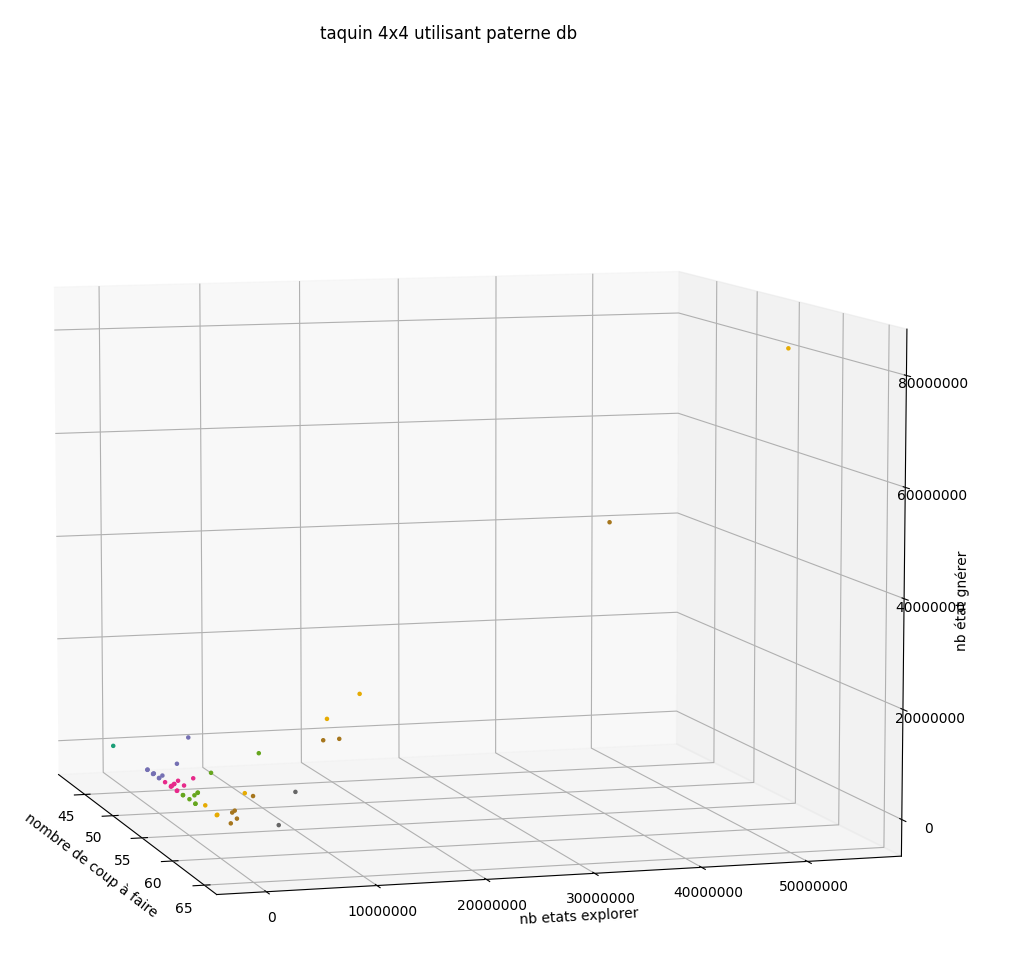
\includegraphics[width=\textwidth]{Taquin 4x4 pa_db graphe 3d}
\end{figure}
\begin{figure}[H]
    \centering
    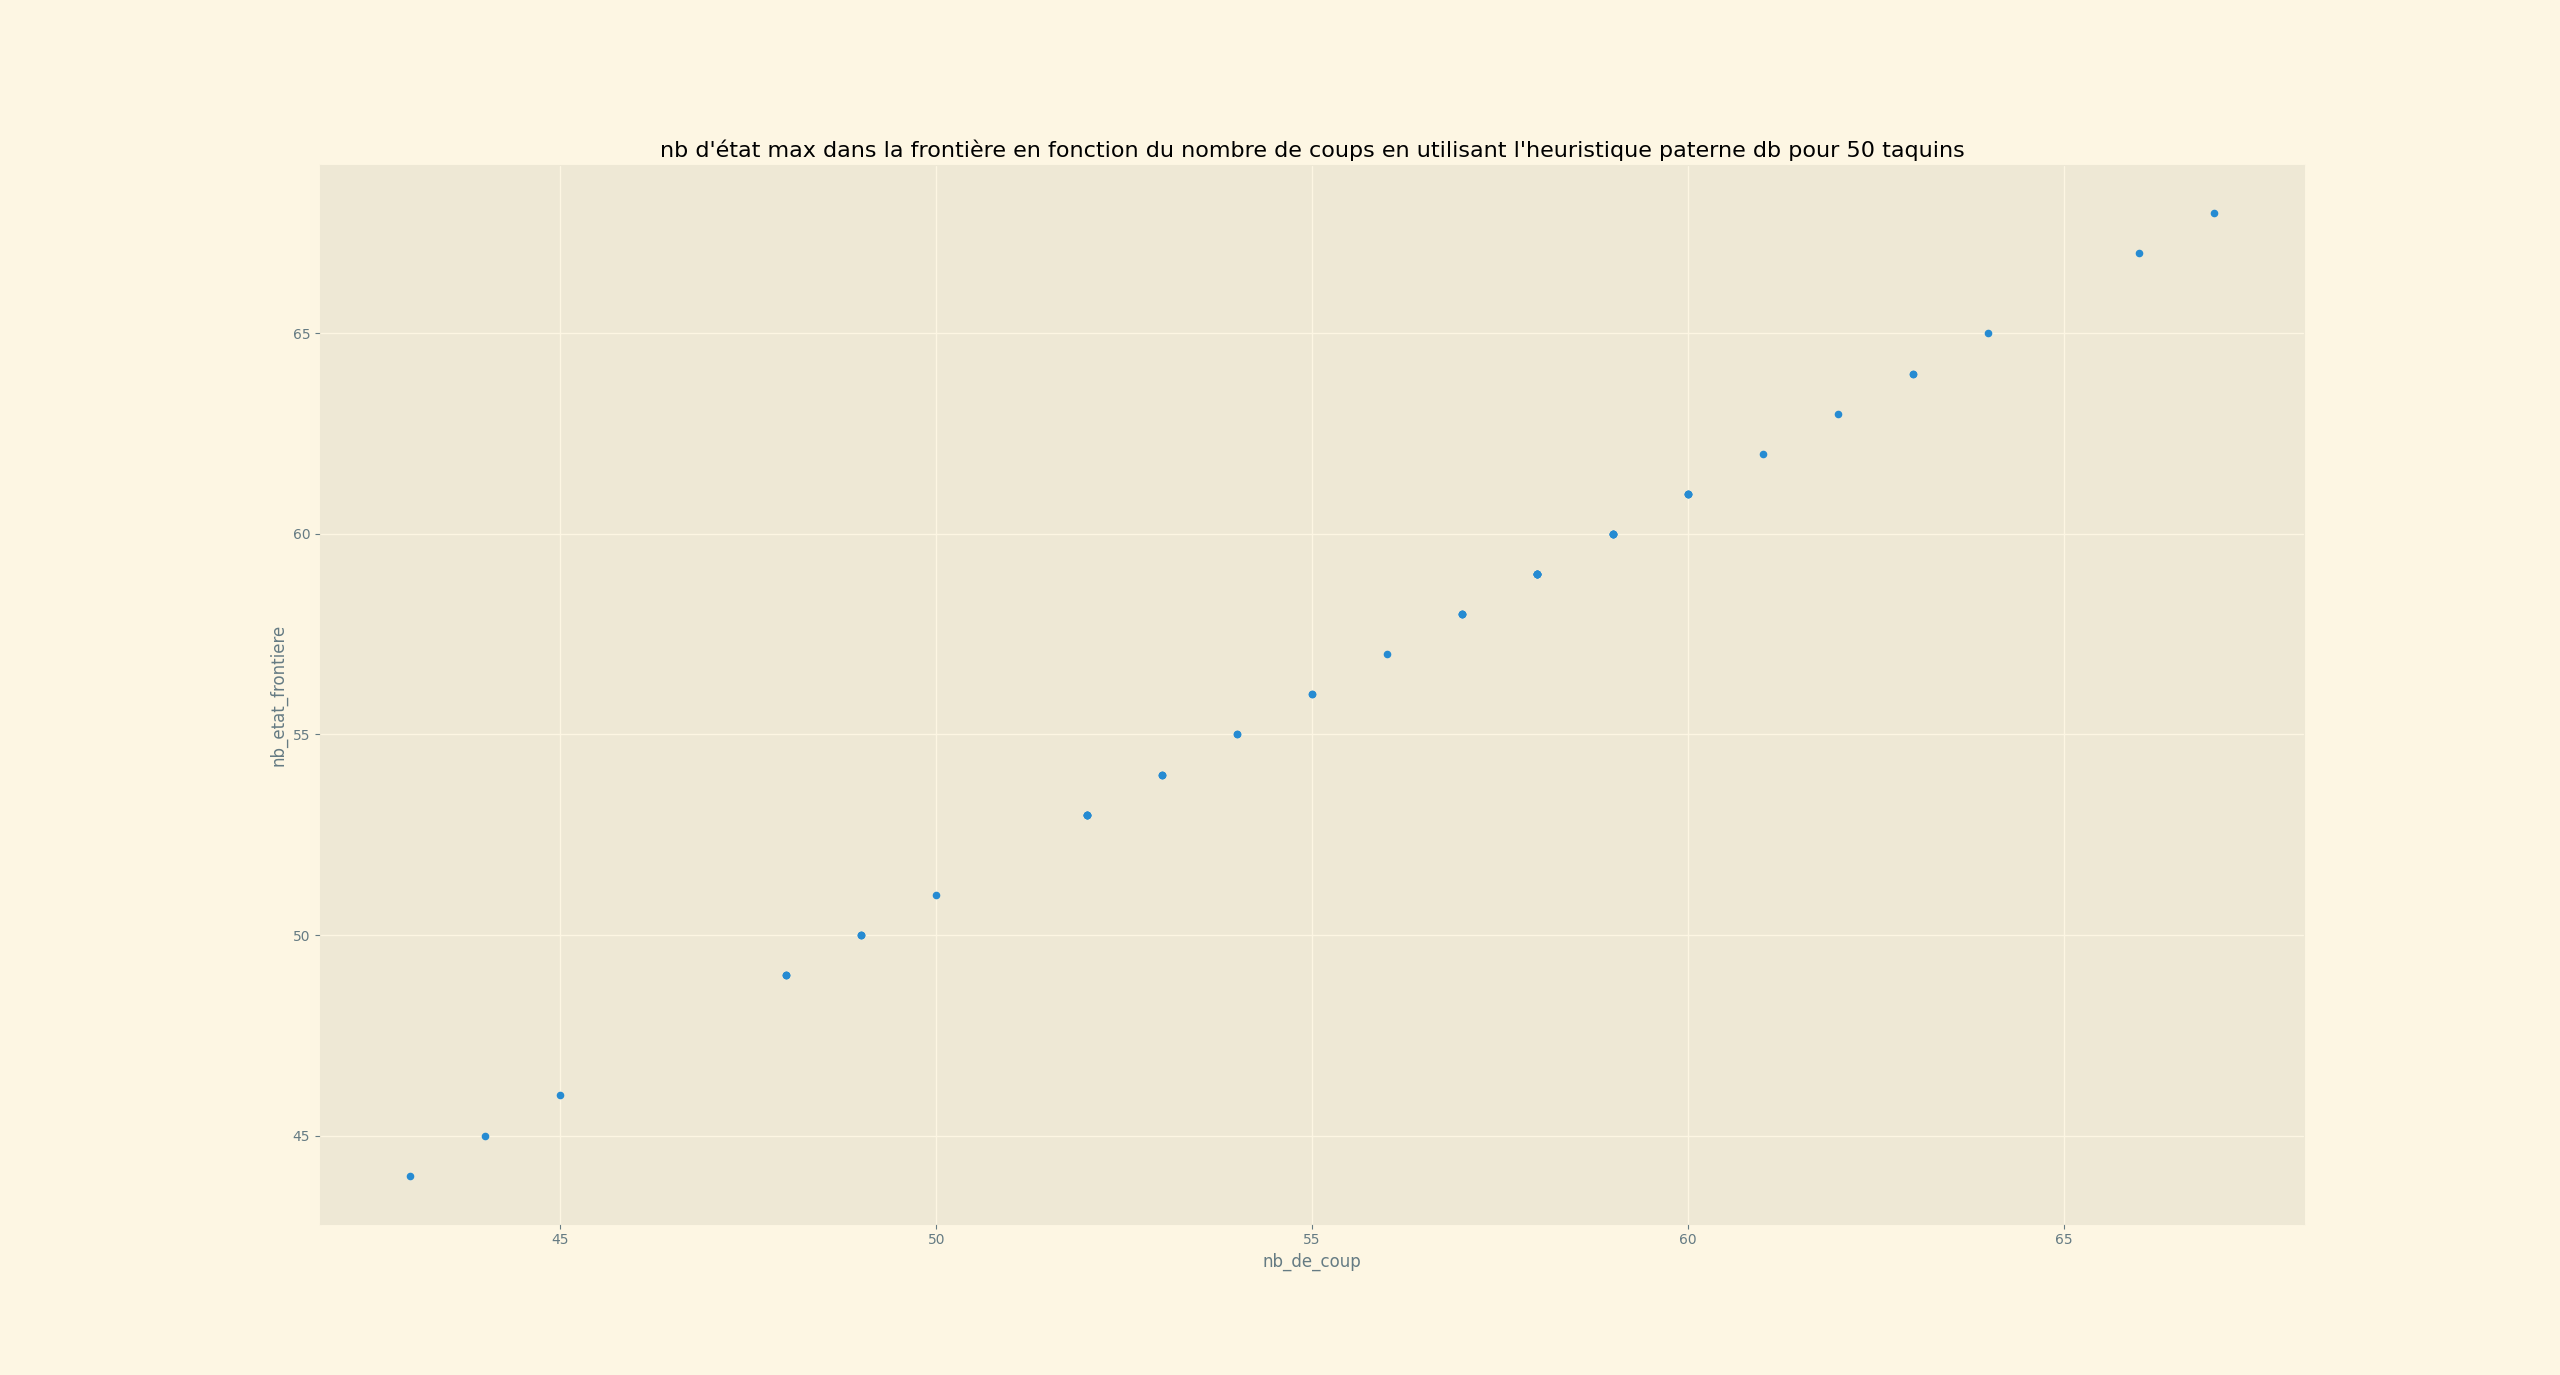
\includegraphics[width=\textwidth]{Taquin 4x4 pa_db nb de etat dans la frontiere en fonction du nb de coups}
\end{figure}
\begin{figure}[H]
    \centering
    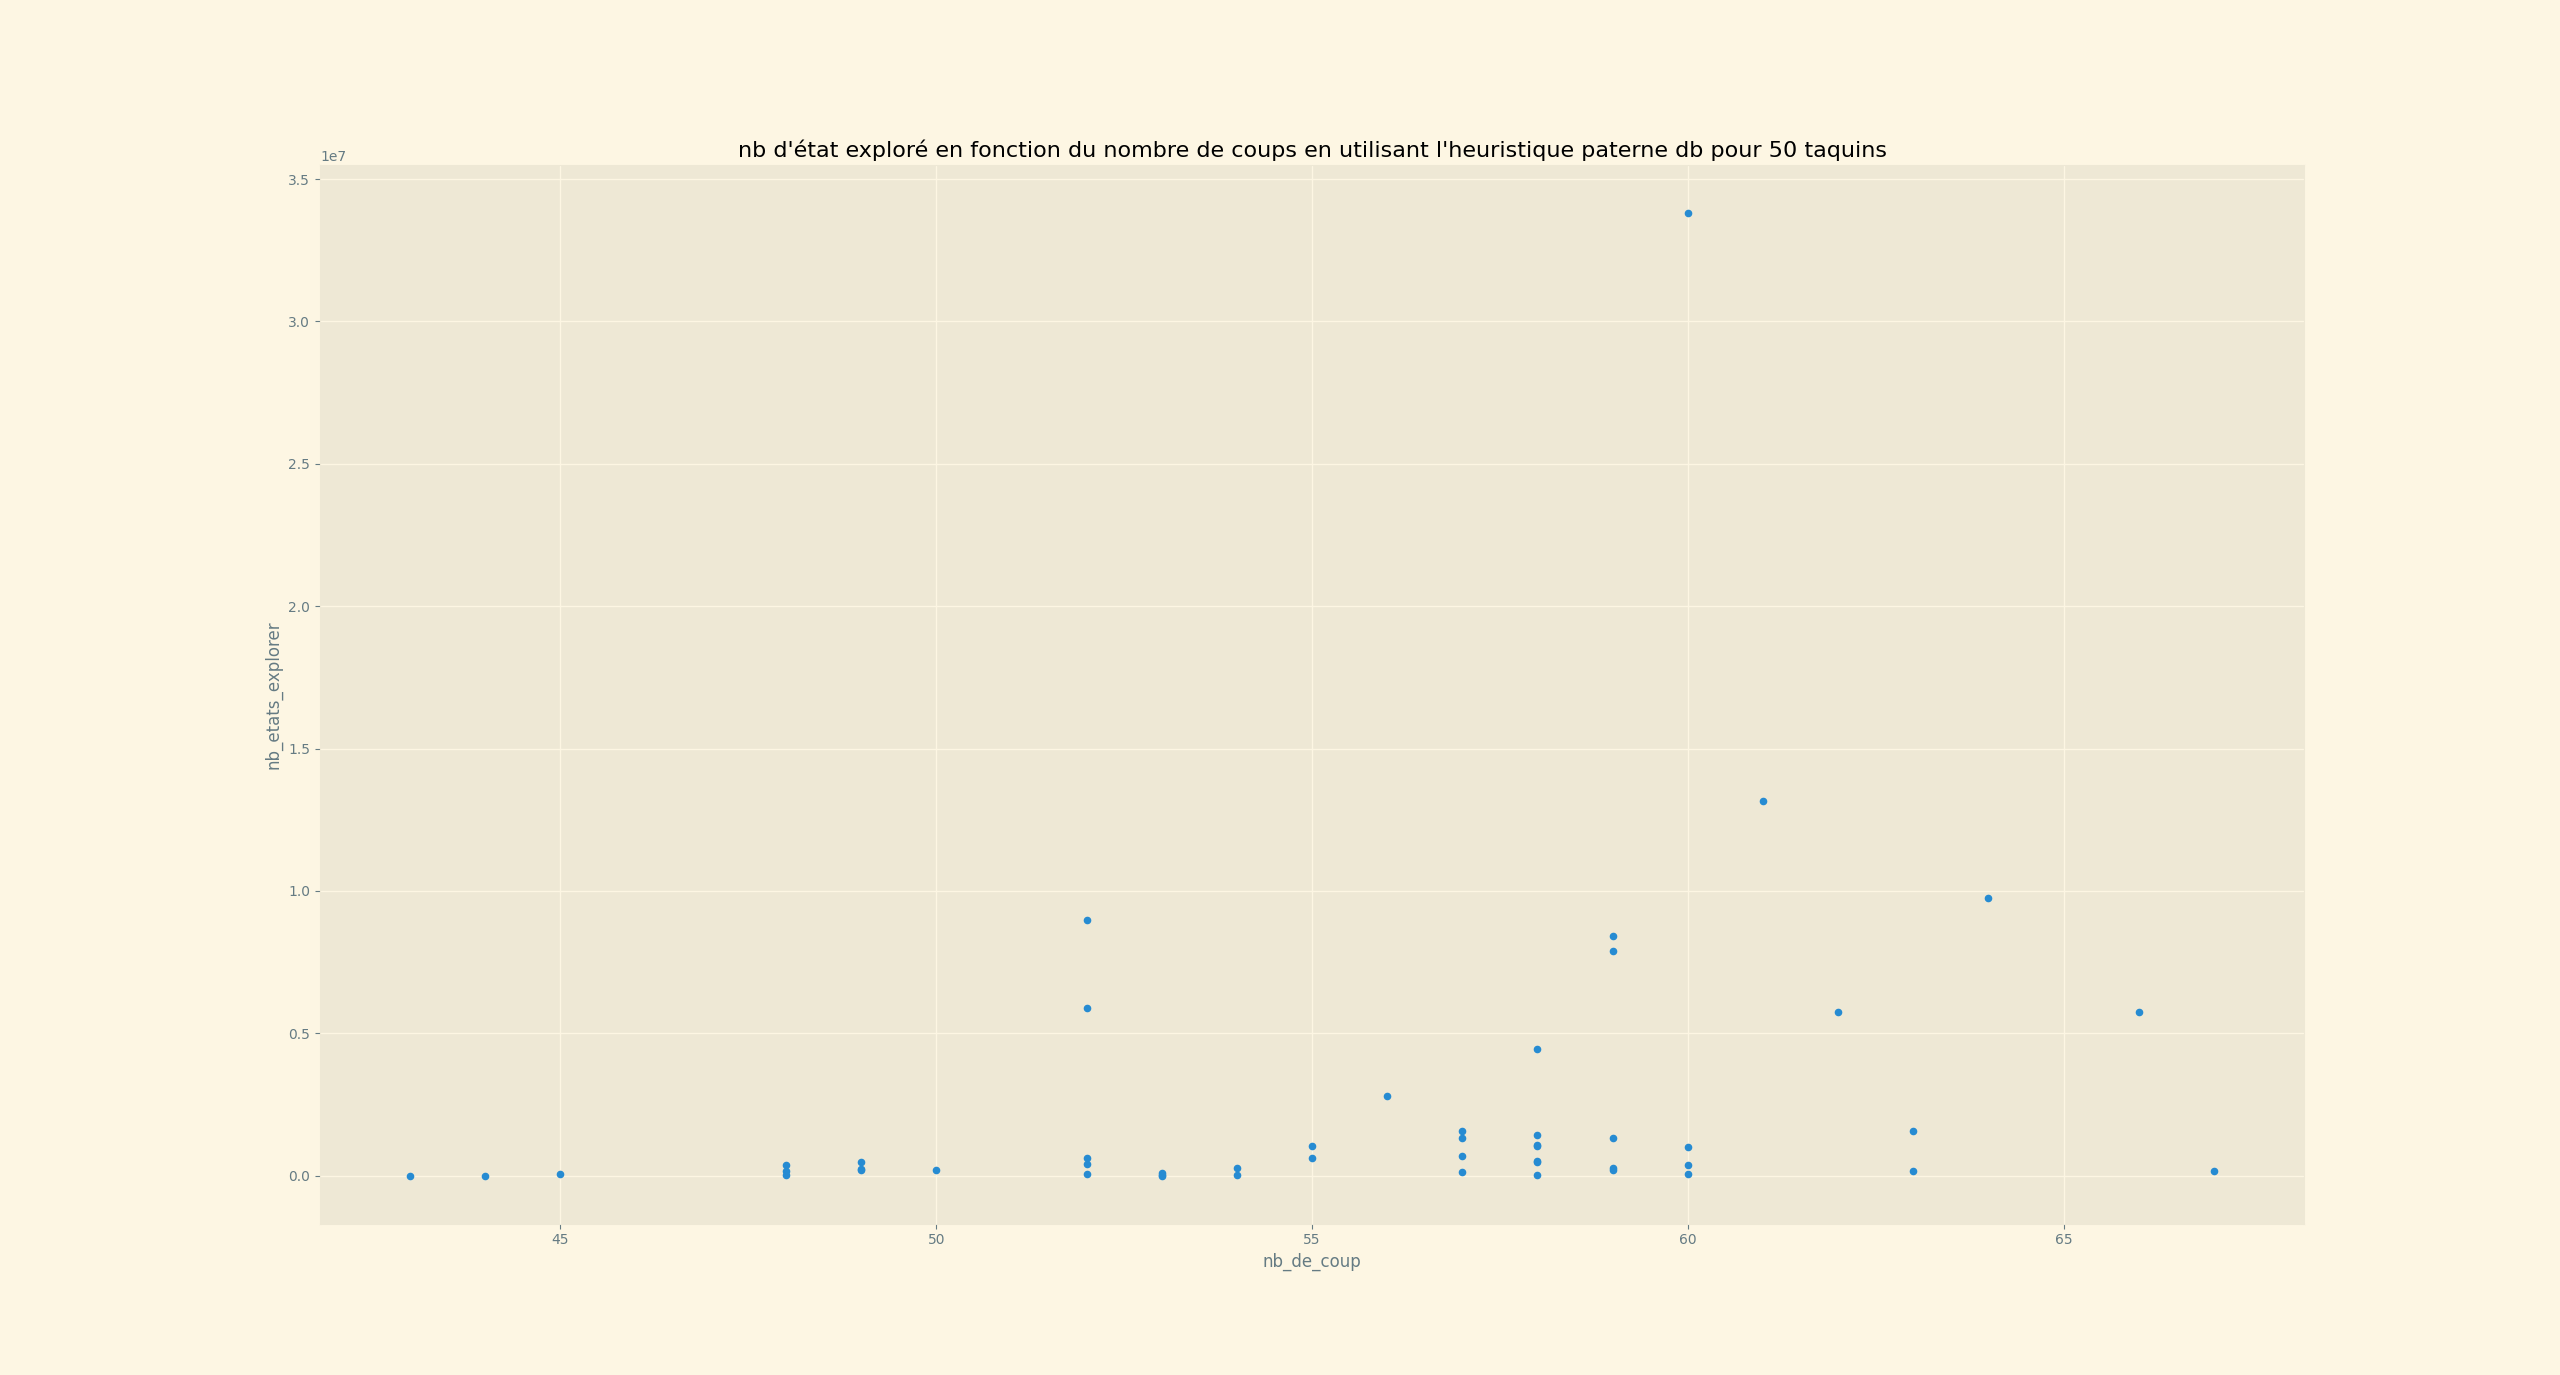
\includegraphics[width=\textwidth]{Taquin 4x4 pa_db nb de noeud exploere en fonction du nombre de coups}
\end{figure}
\begin{figure}[H]
    \centering
    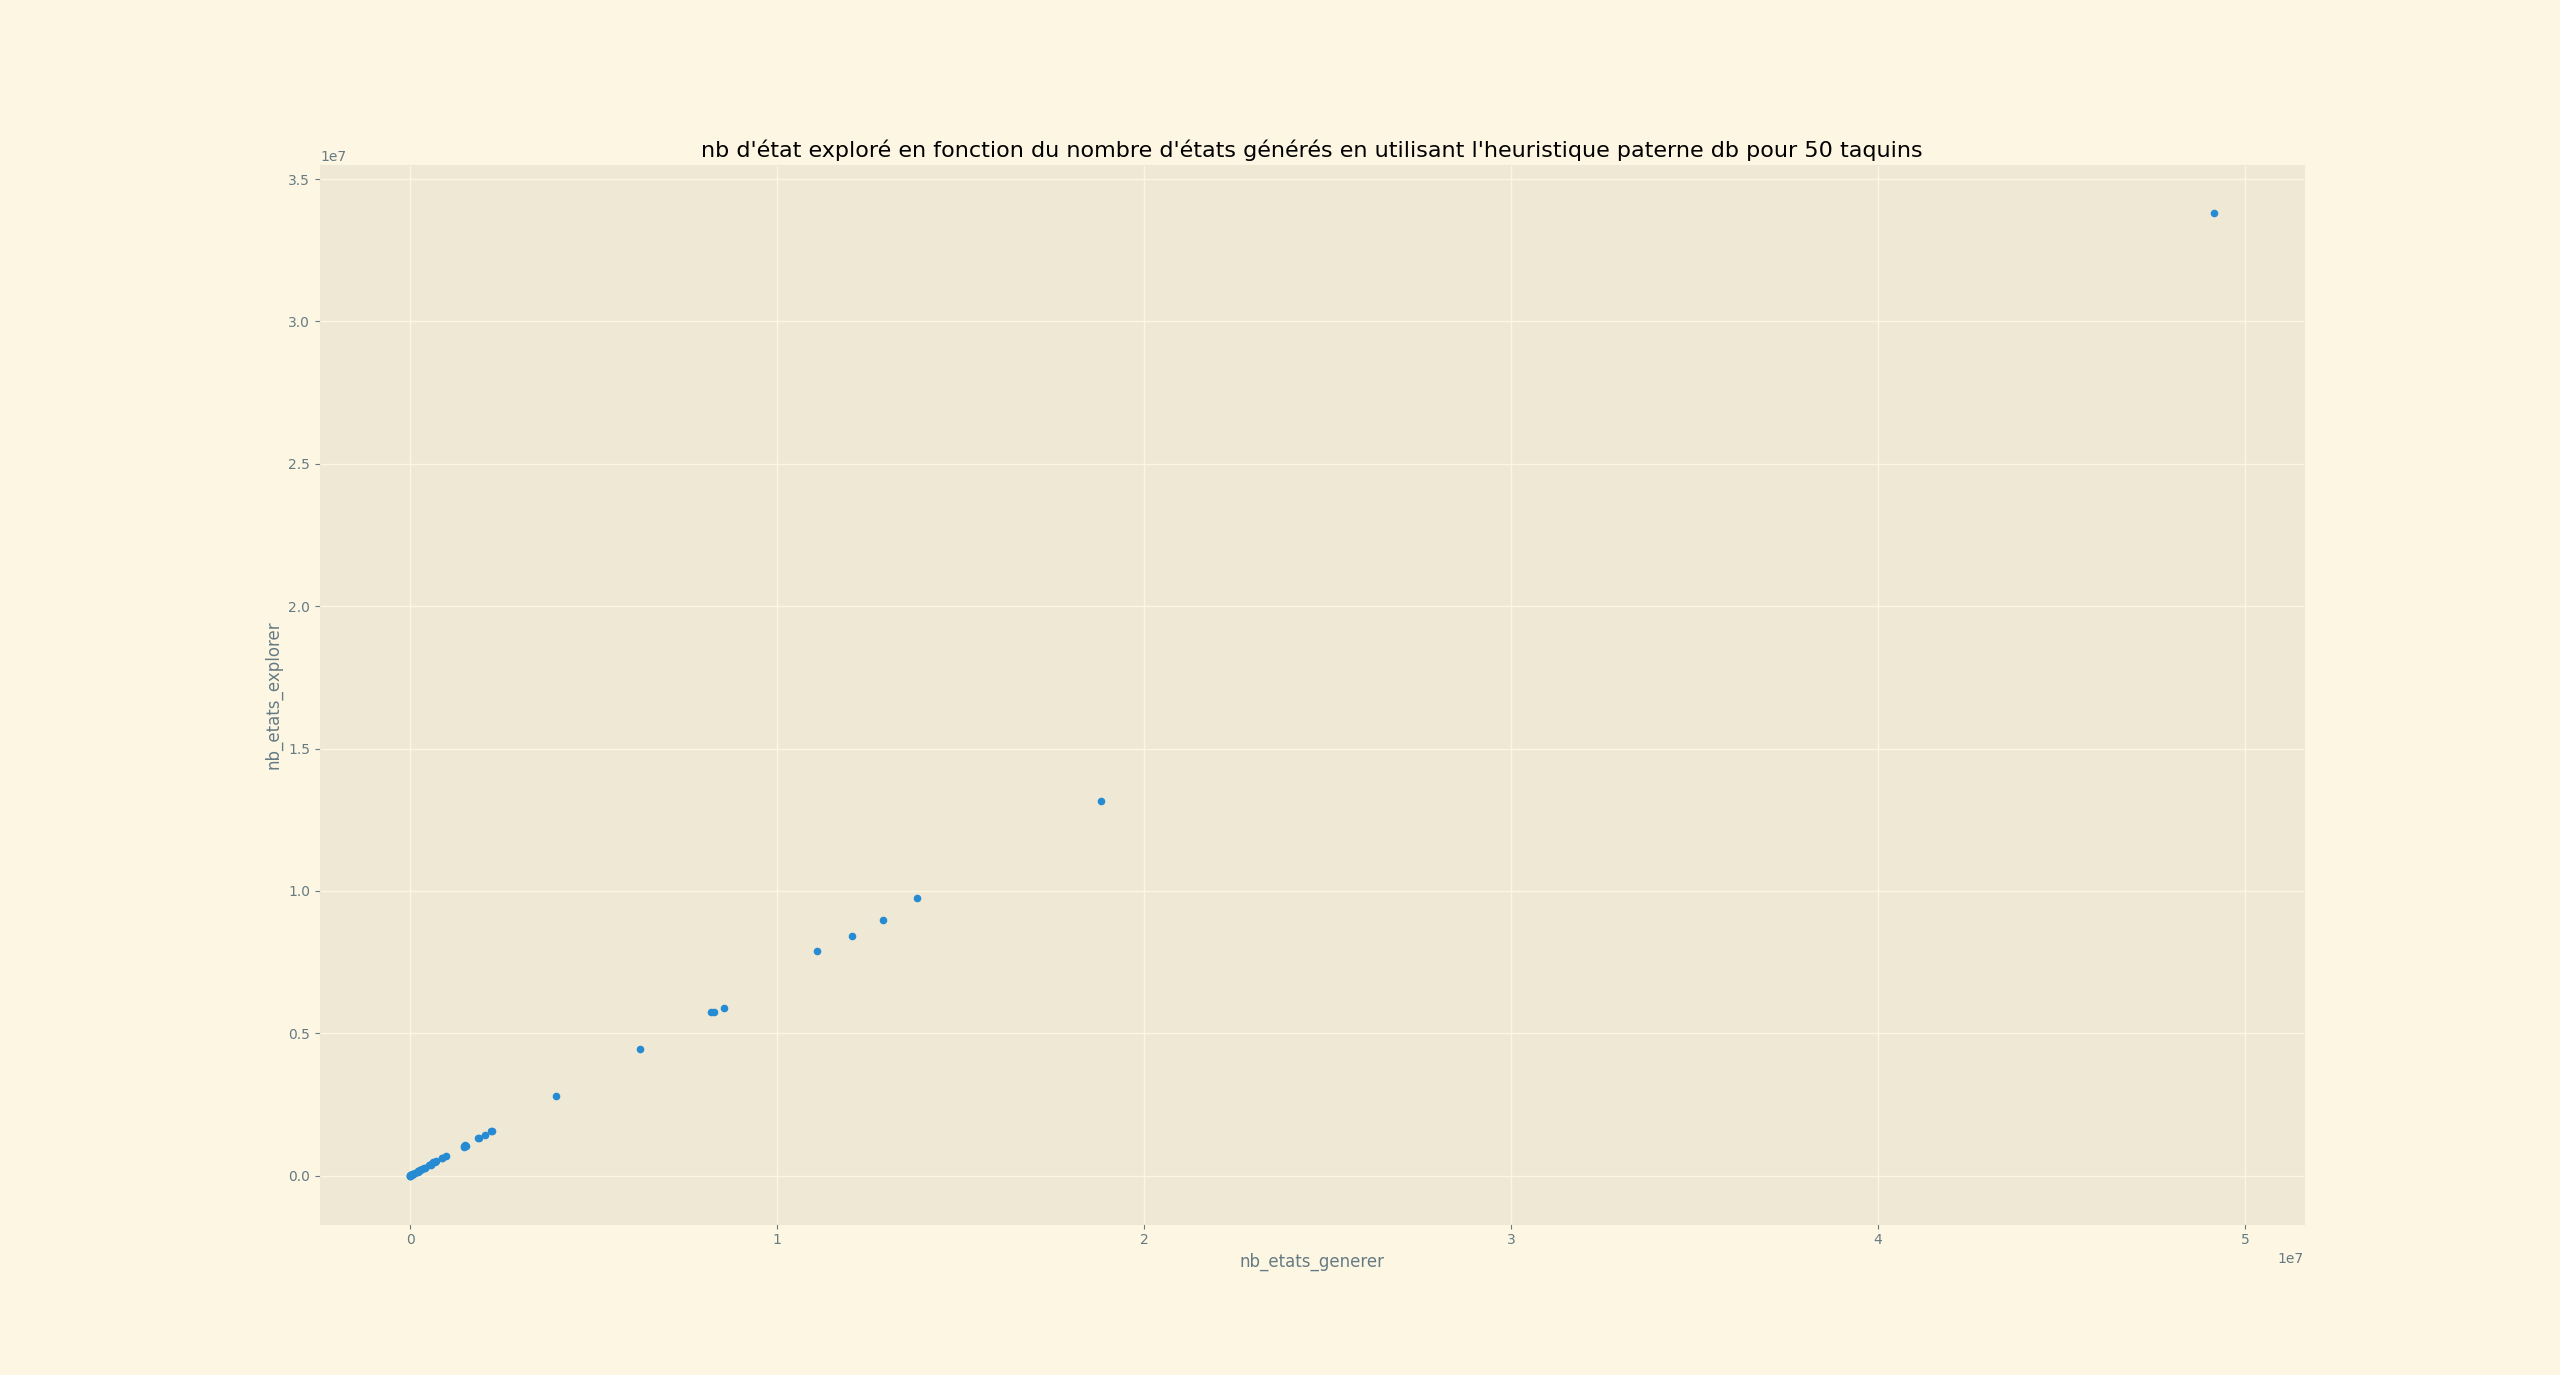
\includegraphics[width=\textwidth]{Taquin 4x4 pa_db nb de noeud explorer en fct du nb detat generer}
\end{figure}
\begin{figure}[H]
    \centering
    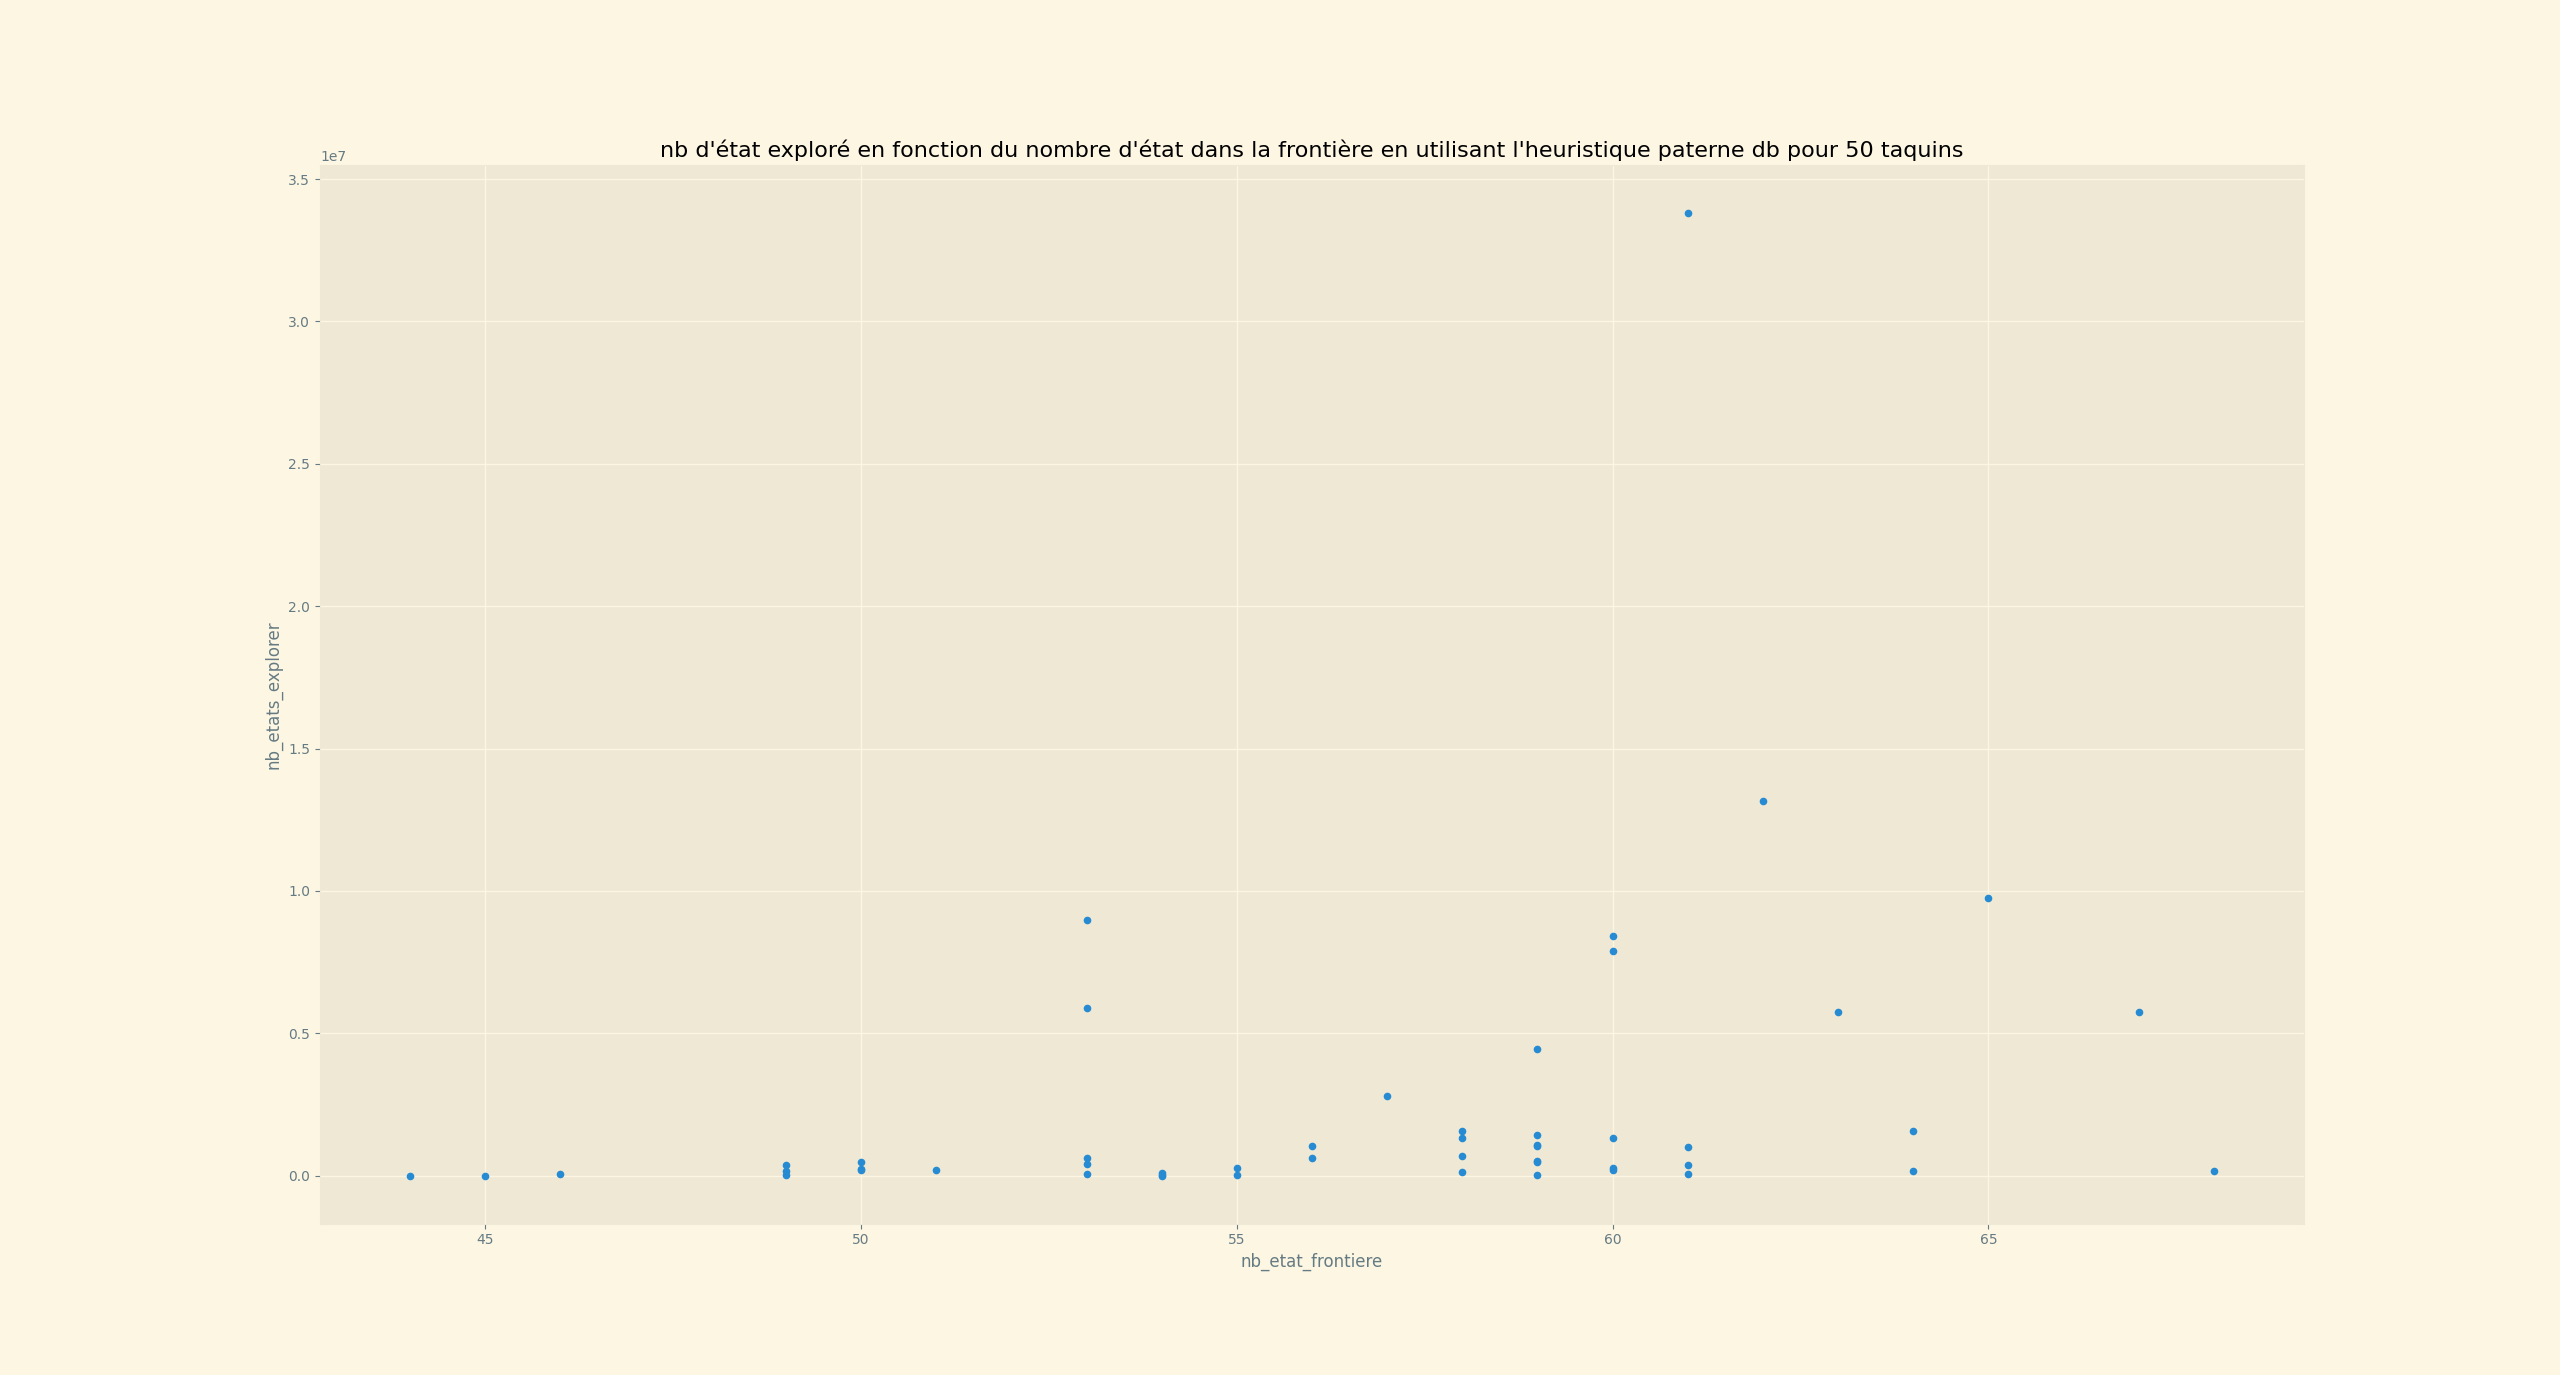
\includegraphics[width=\textwidth]{Taquin 4x4 pa_db nb de noeud explorer en fonction du nombre detat dans la frontiere}
\end{figure}
\begin{figure}[H]
    \centering
    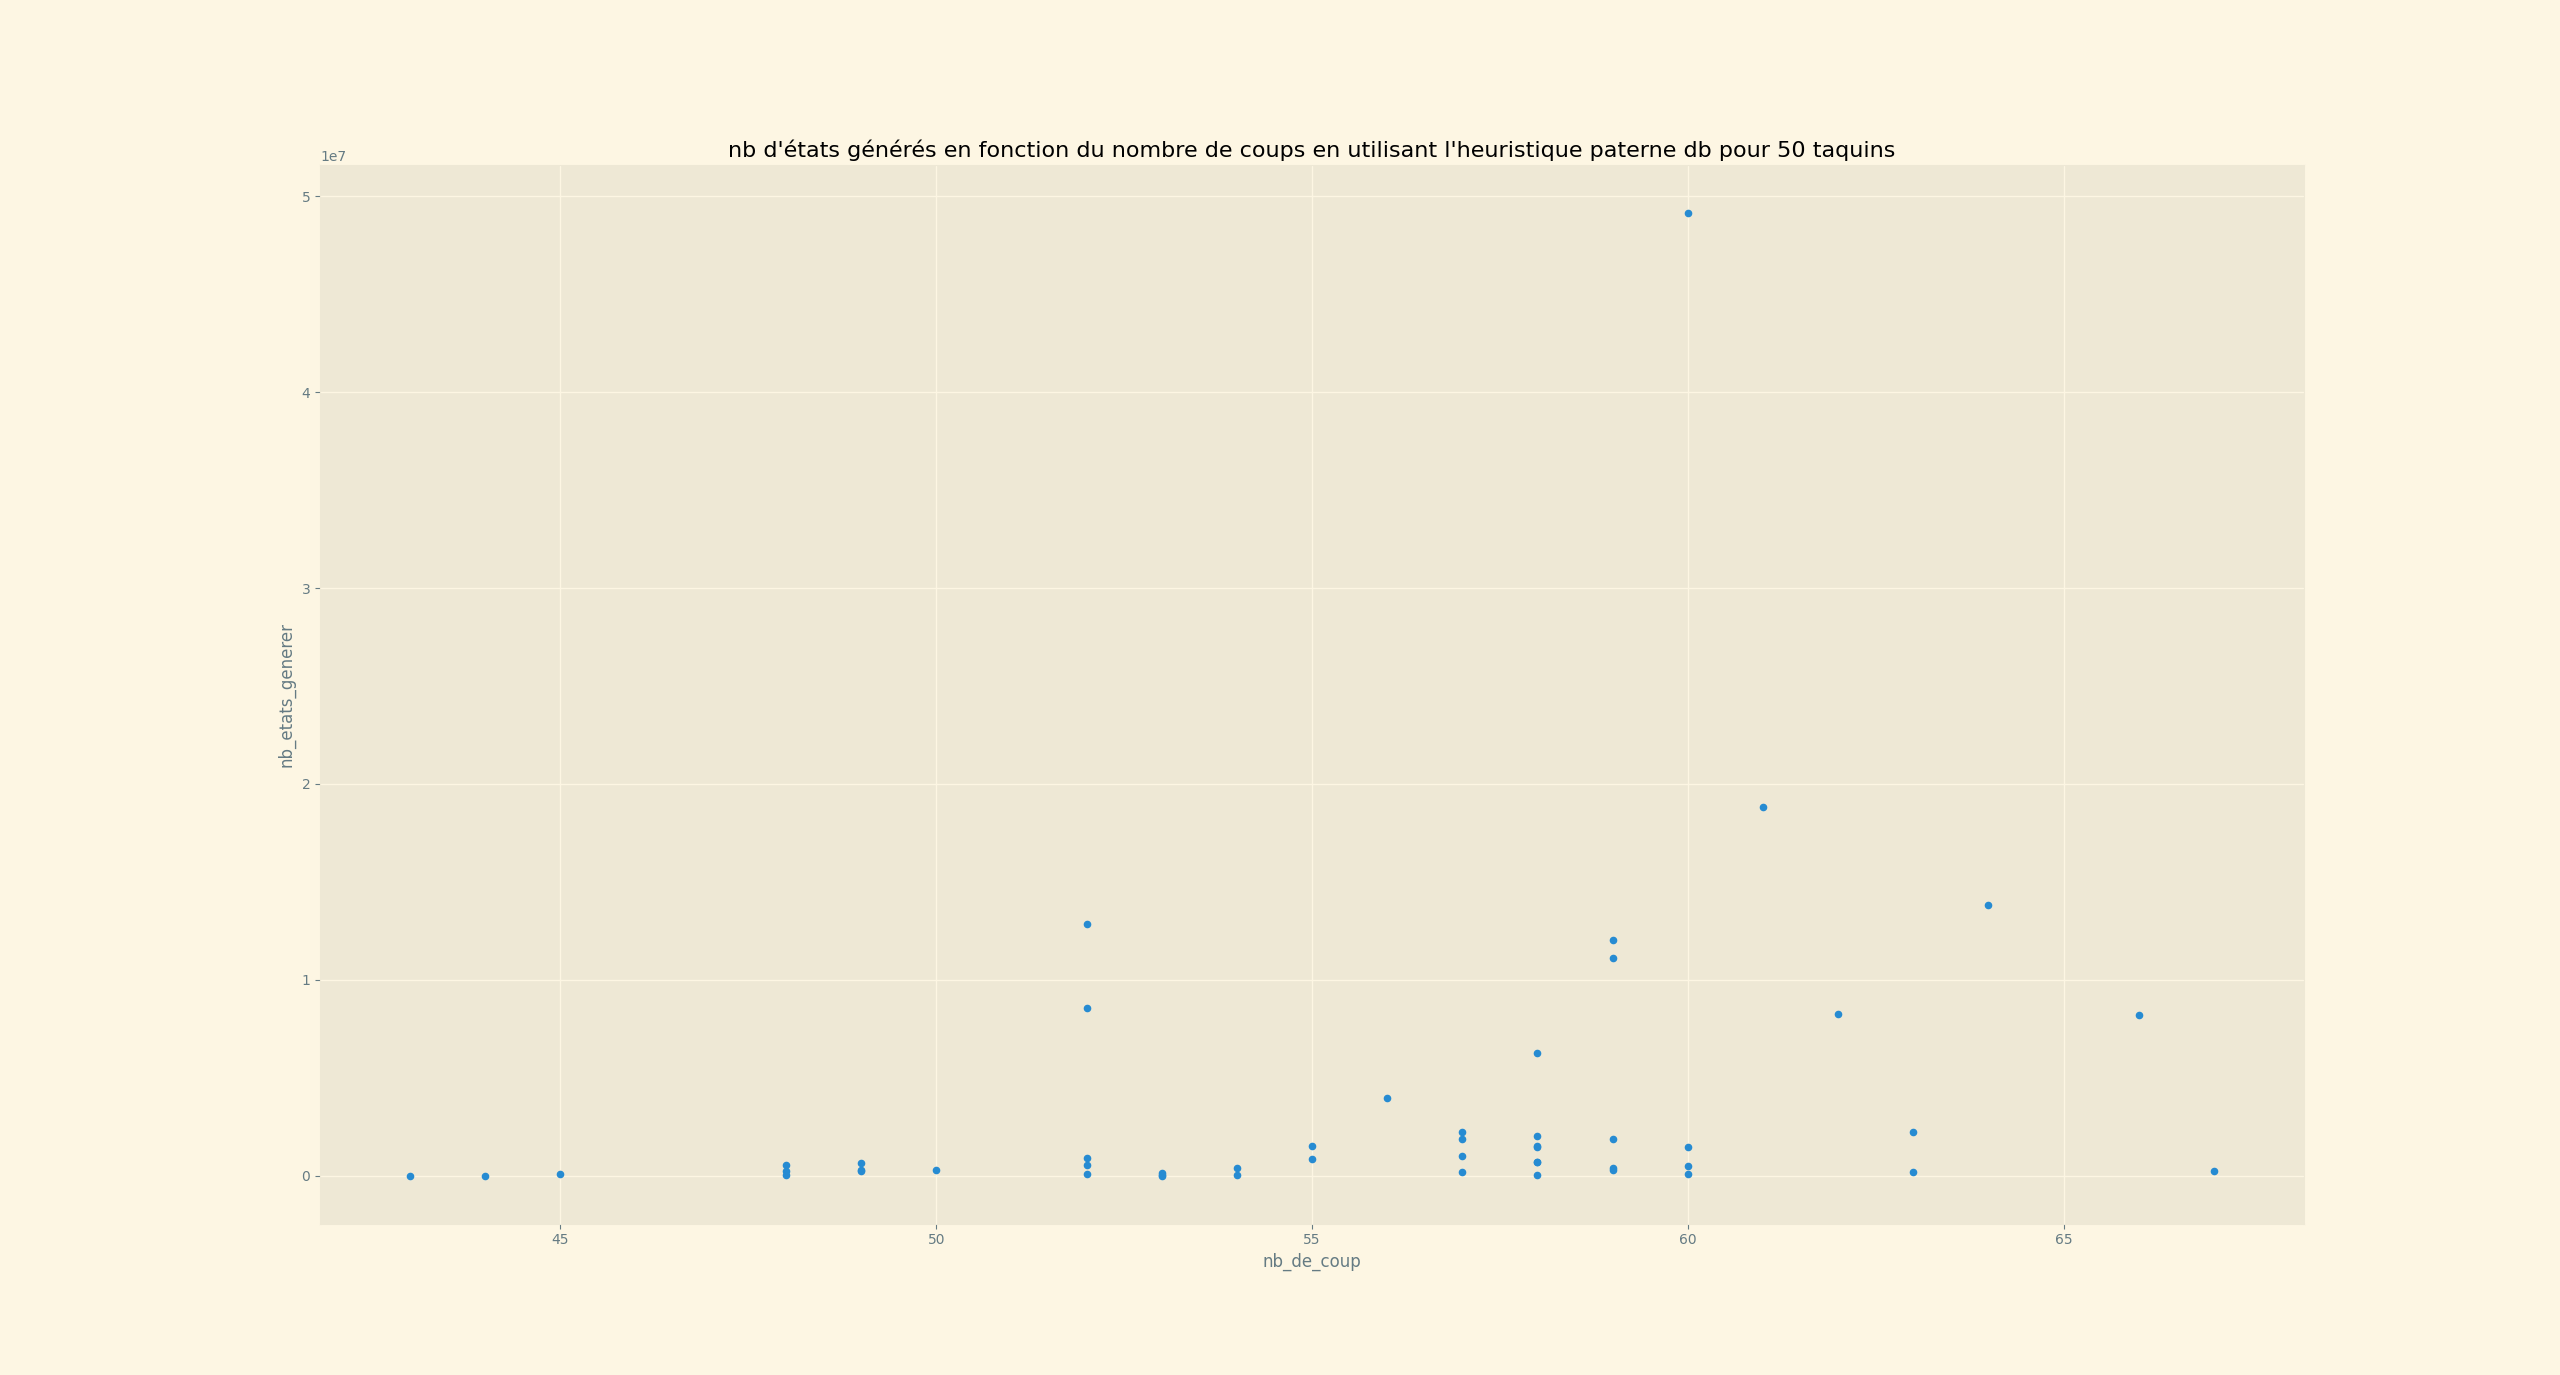
\includegraphics[width=\textwidth]{Taquin 4x4 pa_db nb de noeud noeud generer en fonction du nombre dede coups}
\end{figure}

\begin{tabular}{|l|l|l|}
    \hline
                                   & utilisation de pattern & utilisation de wd \\
    \hline
    nombre de n\oe uds générés     & 2'559                  & 2'996'255         \\
    \hline
    taille max de la frontière     & 47                     & 47                \\
    \hline
    nombre de n\oe uds explorés    & 1893                   & 2'199'469         \\
    \hline
    temps pour trouver la solution & 0.17 s                 & 765.45 s          \\
    \hline
    nombre de coups à réaliser     & 46                     & 46                \\
    \hline
\end{tabular}

\section{Conclusion}
On a pu voir au cours de notre expérimentation que si l'heuristique distance de Manhattan est suffisante pour résoudre facilement des taquins $3 \times 3$, pour des taquins de taille supérieure, cela ne suffisait plus, car l'estimation du coût est peu fiable.

Nous avons donc cherché d'autres heuristiques plus performantes, et nous avons finalement retenu la Walking Distance et le Pattern Database, en combinaison avec l'utilisation de l'algorithme IDA*.

Les deux requièrent de générer en amont une base de données donnant le coût estimé en fonction du schéma de la grille de taquin. Ces bases de données font de quelques Mo pour la Walking distance jusqu'à plusieurs centaines de Mo pour le Pattern Database.

La Walking distance permet d'estimer d'une meilleure manière le coût pour arriver à la solution, en prenant en compte notamment la position de la case vide pour coller au mieux au jeu du taquin. Cette heuristique nous permet de résoudre plus rapidement et plutôt efficacement les taquins $4 \times 4$.

Le Pattern database quant à lui se base sur une bien plus grande collection de patterns de grille pour estimer très précisément le coût pour arriver à la solution de manière très efficace. Avec cette technique, on peut résoudre des taquins difficiles en quelques minutes seulement.

\section{Listing}

Pour des raisons évidentes de papier, tout le code de notre projet est trouvable sur Github : \textbf{https://github.com/YoshiLeLama/projet-taquin}

\end{document}